\documentclass[twoside]{book}

% Packages required by doxygen
\usepackage{fixltx2e}
\usepackage{calc}
\usepackage{doxygen}
\usepackage[export]{adjustbox} % also loads graphicx
\usepackage{graphicx}
\usepackage[utf8]{inputenc}
\usepackage{makeidx}
\usepackage{multicol}
\usepackage{multirow}
\PassOptionsToPackage{warn}{textcomp}
\usepackage{textcomp}
\usepackage[nointegrals]{wasysym}
\usepackage[table]{xcolor}

% Font selection
\usepackage[T1]{fontenc}
\usepackage[scaled=.90]{helvet}
\usepackage{courier}
\usepackage{amssymb}
\usepackage{sectsty}
\renewcommand{\familydefault}{\sfdefault}
\allsectionsfont{%
  \fontseries{bc}\selectfont%
  \color{darkgray}%
}
\renewcommand{\DoxyLabelFont}{%
  \fontseries{bc}\selectfont%
  \color{darkgray}%
}
\newcommand{\+}{\discretionary{\mbox{\scriptsize$\hookleftarrow$}}{}{}}

% Page & text layout
\usepackage{geometry}
\geometry{%
  a4paper,%
  top=2.5cm,%
  bottom=2.5cm,%
  left=2.5cm,%
  right=2.5cm%
}
\tolerance=750
\hfuzz=15pt
\hbadness=750
\setlength{\emergencystretch}{15pt}
\setlength{\parindent}{0cm}
\setlength{\parskip}{3ex plus 2ex minus 2ex}
\makeatletter
\renewcommand{\paragraph}{%
  \@startsection{paragraph}{4}{0ex}{-1.0ex}{1.0ex}{%
    \normalfont\normalsize\bfseries\SS@parafont%
  }%
}
\renewcommand{\subparagraph}{%
  \@startsection{subparagraph}{5}{0ex}{-1.0ex}{1.0ex}{%
    \normalfont\normalsize\bfseries\SS@subparafont%
  }%
}
\makeatother

% Headers & footers
\usepackage{fancyhdr}
\pagestyle{fancyplain}
\fancyhead[LE]{\fancyplain{}{\bfseries\thepage}}
\fancyhead[CE]{\fancyplain{}{}}
\fancyhead[RE]{\fancyplain{}{\bfseries\leftmark}}
\fancyhead[LO]{\fancyplain{}{\bfseries\rightmark}}
\fancyhead[CO]{\fancyplain{}{}}
\fancyhead[RO]{\fancyplain{}{\bfseries\thepage}}
\fancyfoot[LE]{\fancyplain{}{}}
\fancyfoot[CE]{\fancyplain{}{}}
\fancyfoot[RE]{\fancyplain{}{\bfseries\scriptsize Generated by Doxygen }}
\fancyfoot[LO]{\fancyplain{}{\bfseries\scriptsize Generated by Doxygen }}
\fancyfoot[CO]{\fancyplain{}{}}
\fancyfoot[RO]{\fancyplain{}{}}
\renewcommand{\footrulewidth}{0.4pt}
\renewcommand{\chaptermark}[1]{%
  \markboth{#1}{}%
}
\renewcommand{\sectionmark}[1]{%
  \markright{\thesection\ #1}%
}

% Indices & bibliography
\usepackage{natbib}
\usepackage[titles]{tocloft}
\setcounter{tocdepth}{3}
\setcounter{secnumdepth}{5}
\makeindex

% Hyperlinks (required, but should be loaded last)
\usepackage{ifpdf}
\ifpdf
  \usepackage[pdftex,pagebackref=true]{hyperref}
\else
  \usepackage[ps2pdf,pagebackref=true]{hyperref}
\fi
\hypersetup{%
  colorlinks=true,%
  linkcolor=blue,%
  citecolor=blue,%
  unicode%
}

% Custom commands
\newcommand{\clearemptydoublepage}{%
  \newpage{\pagestyle{empty}\cleardoublepage}%
}

\usepackage{caption}
\captionsetup{labelsep=space,justification=centering,font={bf},singlelinecheck=off,skip=4pt,position=top}

%===== C O N T E N T S =====

\begin{document}

% Titlepage & ToC
\hypersetup{pageanchor=false,
             bookmarksnumbered=true,
             pdfencoding=unicode
            }
\pagenumbering{alph}
\begin{titlepage}
\vspace*{7cm}
\begin{center}%
{\Large My Project \\[1ex]\large 1.\+1 }\\
\vspace*{1cm}
{\large Generated by Doxygen 1.8.14}\\
\end{center}
\end{titlepage}
\clearemptydoublepage
\pagenumbering{roman}
\tableofcontents
\clearemptydoublepage
\pagenumbering{arabic}
\hypersetup{pageanchor=true}

%--- Begin generated contents ---
\chapter{Namespace Index}
\section{Namespace List}
Here is a list of all documented namespaces with brief descriptions\+:\begin{DoxyCompactList}
\item\contentsline{section}{\mbox{\hyperlink{namespacegrman}{grman}} }{\pageref{namespacegrman}}{}
\end{DoxyCompactList}

\chapter{Hierarchical Index}
\section{Class Hierarchy}
This inheritance list is sorted roughly, but not completely, alphabetically\+:\begin{DoxyCompactList}
\item \contentsline{section}{grman\+:\+:Arrow\+Item}{\pageref{structgrman_1_1_arrow_item}}{}
\item \contentsline{section}{Coords}{\pageref{struct_coords}}{}
\item \contentsline{section}{Edge}{\pageref{class_edge}}{}
\item \contentsline{section}{Edge\+Interface}{\pageref{class_edge_interface}}{}
\item \contentsline{section}{Frame}{\pageref{struct_frame}}{}
\item \contentsline{section}{Graph}{\pageref{class_graph}}{}
\item \contentsline{section}{Graphe\+Interface}{\pageref{class_graphe_interface}}{}
\item \contentsline{section}{Graph\+Interface}{\pageref{class_graph_interface}}{}
\item \contentsline{section}{Vertex}{\pageref{class_vertex}}{}
\item \contentsline{section}{Vertex\+Interface}{\pageref{class_vertex_interface}}{}
\item \contentsline{section}{grman\+:\+:Widget}{\pageref{classgrman_1_1_widget}}{}
\begin{DoxyCompactList}
\item \contentsline{section}{grman\+:\+:Widget\+Box}{\pageref{classgrman_1_1_widget_box}}{}
\item \contentsline{section}{grman\+:\+:Widget\+Button}{\pageref{classgrman_1_1_widget_button}}{}
\item \contentsline{section}{grman\+:\+:Widget\+Check\+Box}{\pageref{classgrman_1_1_widget_check_box}}{}
\item \contentsline{section}{grman\+:\+:Widget\+Edge}{\pageref{classgrman_1_1_widget_edge}}{}
\item \contentsline{section}{grman\+:\+:Widget\+Image}{\pageref{classgrman_1_1_widget_image}}{}
\item \contentsline{section}{grman\+:\+:Widget\+Text}{\pageref{classgrman_1_1_widget_text}}{}
\item \contentsline{section}{grman\+:\+:Widget\+V\+Slider}{\pageref{classgrman_1_1_widget_v_slider}}{}
\end{DoxyCompactList}
\end{DoxyCompactList}

\chapter{Class Index}
\section{Class List}
Here are the classes, structs, unions and interfaces with brief descriptions\+:\begin{DoxyCompactList}
\item\contentsline{section}{\mbox{\hyperlink{structgrman_1_1_arrow_item}{grman\+::\+Arrow\+Item}} }{\pageref{structgrman_1_1_arrow_item}}{}
\item\contentsline{section}{\mbox{\hyperlink{struct_coords}{Coords}} }{\pageref{struct_coords}}{}
\item\contentsline{section}{\mbox{\hyperlink{class_edge}{Edge}} \\*Classe representant les arcs du graphe }{\pageref{class_edge}}{}
\item\contentsline{section}{\mbox{\hyperlink{class_edge_interface}{Edge\+Interface}} \\*Classe representant l\textquotesingle{}interface graphique des arcs du graphe }{\pageref{class_edge_interface}}{}
\item\contentsline{section}{\mbox{\hyperlink{struct_frame}{Frame}} }{\pageref{struct_frame}}{}
\item\contentsline{section}{\mbox{\hyperlink{class_graph}{Graph}} \\*Classe representant le graphe }{\pageref{class_graph}}{}
\item\contentsline{section}{\mbox{\hyperlink{class_graphe_interface}{Graphe\+Interface}} \\*Classe representant l\textquotesingle{}interface graphique du graphe }{\pageref{class_graphe_interface}}{}
\item\contentsline{section}{\mbox{\hyperlink{class_graph_interface}{Graph\+Interface}} }{\pageref{class_graph_interface}}{}
\item\contentsline{section}{\mbox{\hyperlink{class_vertex}{Vertex}} \\*Classe representant les sommets du graphe }{\pageref{class_vertex}}{}
\item\contentsline{section}{\mbox{\hyperlink{class_vertex_interface}{Vertex\+Interface}} \\*Classe representant l\textquotesingle{}interface graphique des sommets }{\pageref{class_vertex_interface}}{}
\item\contentsline{section}{\mbox{\hyperlink{classgrman_1_1_widget}{grman\+::\+Widget}} }{\pageref{classgrman_1_1_widget}}{}
\item\contentsline{section}{\mbox{\hyperlink{classgrman_1_1_widget_box}{grman\+::\+Widget\+Box}} }{\pageref{classgrman_1_1_widget_box}}{}
\item\contentsline{section}{\mbox{\hyperlink{classgrman_1_1_widget_button}{grman\+::\+Widget\+Button}} }{\pageref{classgrman_1_1_widget_button}}{}
\item\contentsline{section}{\mbox{\hyperlink{classgrman_1_1_widget_check_box}{grman\+::\+Widget\+Check\+Box}} }{\pageref{classgrman_1_1_widget_check_box}}{}
\item\contentsline{section}{\mbox{\hyperlink{classgrman_1_1_widget_edge}{grman\+::\+Widget\+Edge}} }{\pageref{classgrman_1_1_widget_edge}}{}
\item\contentsline{section}{\mbox{\hyperlink{classgrman_1_1_widget_image}{grman\+::\+Widget\+Image}} }{\pageref{classgrman_1_1_widget_image}}{}
\item\contentsline{section}{\mbox{\hyperlink{classgrman_1_1_widget_text}{grman\+::\+Widget\+Text}} \\*Extr�mement rudimentaire \+: � compl�ter ! }{\pageref{classgrman_1_1_widget_text}}{}
\item\contentsline{section}{\mbox{\hyperlink{classgrman_1_1_widget_v_slider}{grman\+::\+Widget\+V\+Slider}} }{\pageref{classgrman_1_1_widget_v_slider}}{}
\end{DoxyCompactList}

\chapter{File Index}
\section{File List}
Here is a list of all documented files with brief descriptions\+:\begin{DoxyCompactList}
\item\contentsline{section}{{\bfseries Acceuil1.\+cpp} }{\pageref{_acceuil1_8cpp}}{}
\item\contentsline{section}{{\bfseries Acceuil1.\+h} }{\pageref{_acceuil1_8h}}{}
\item\contentsline{section}{{\bfseries Acceuil2.\+cpp} }{\pageref{_acceuil2_8cpp}}{}
\item\contentsline{section}{{\bfseries Acceuil2.\+h} }{\pageref{_acceuil2_8h}}{}
\item\contentsline{section}{{\bfseries Analyse1.\+cpp} }{\pageref{_analyse1_8cpp}}{}
\item\contentsline{section}{{\bfseries Analyse1.\+h} }{\pageref{_analyse1_8h}}{}
\item\contentsline{section}{{\bfseries Analyse\+\_\+\+F\+\_\+\+C.\+cpp} }{\pageref{_analyse___f___c_8cpp}}{}
\item\contentsline{section}{{\bfseries Analyse\+\_\+\+F\+\_\+\+C.\+h} }{\pageref{_analyse___f___c_8h}}{}
\item\contentsline{section}{{\bfseries analyse\+\_\+\+K\+\_\+\+C.\+cpp} }{\pageref{analyse___k___c_8cpp}}{}
\item\contentsline{section}{{\bfseries analyse\+\_\+\+K\+\_\+\+C.\+h} }{\pageref{analyse___k___c_8h}}{}
\item\contentsline{section}{\mbox{\hyperlink{_edge_8cpp}{Edge.\+cpp}} \\*Cr�ation d\textquotesingle{}un �cosyst�me }{\pageref{_edge_8cpp}}{}
\item\contentsline{section}{\mbox{\hyperlink{_edge_8h}{Edge.\+h}} \\*Cr�ation d\textquotesingle{}un �cosyst�me }{\pageref{_edge_8h}}{}
\item\contentsline{section}{\mbox{\hyperlink{_edge_interface_8cpp}{Edge\+Interface.\+cpp}} \\*Cr�ation d\textquotesingle{}un �cosyst�me }{\pageref{_edge_interface_8cpp}}{}
\item\contentsline{section}{\mbox{\hyperlink{_edge_interface_8h}{Edge\+Interface.\+h}} \\*Cr�ation d\textquotesingle{}un �cosyst�me }{\pageref{_edge_interface_8h}}{}
\item\contentsline{section}{\mbox{\hyperlink{graph_8cpp}{graph.\+cpp}} \\*Cr�ation d\textquotesingle{}un �cosyst�me }{\pageref{graph_8cpp}}{}
\item\contentsline{section}{\mbox{\hyperlink{graph_8h}{graph.\+h}} \\*Cr�ation d\textquotesingle{}un �cosyst�me }{\pageref{graph_8h}}{}
\item\contentsline{section}{\mbox{\hyperlink{_graphe_interface_8cpp}{Graphe\+Interface.\+cpp}} \\*Cr�ation d\textquotesingle{}un �cosyst�me }{\pageref{_graphe_interface_8cpp}}{}
\item\contentsline{section}{\mbox{\hyperlink{_graphe_interface_8h}{Graphe\+Interface.\+h}} \\*Cr�ation d\textquotesingle{}un �cosyst�me }{\pageref{_graphe_interface_8h}}{}
\item\contentsline{section}{\mbox{\hyperlink{main_8cpp}{main.\+cpp}} \\*Cr�ation d\textquotesingle{}un �cosyst�me }{\pageref{main_8cpp}}{}
\item\contentsline{section}{{\bfseries Manuel.\+cpp} }{\pageref{_manuel_8cpp}}{}
\item\contentsline{section}{{\bfseries Manuel.\+h} }{\pageref{_manuel_8h}}{}
\item\contentsline{section}{{\bfseries Menu1.\+cpp} }{\pageref{_menu1_8cpp}}{}
\item\contentsline{section}{{\bfseries Menu1.\+h} }{\pageref{_menu1_8h}}{}
\item\contentsline{section}{{\bfseries Simulation.\+cpp} }{\pageref{_simulation_8cpp}}{}
\item\contentsline{section}{{\bfseries Simulation.\+h} }{\pageref{_simulation_8h}}{}
\item\contentsline{section}{\mbox{\hyperlink{_vertex_8cpp}{Vertex.\+cpp}} \\*Cr�ation d\textquotesingle{}un �cosyst�me }{\pageref{_vertex_8cpp}}{}
\item\contentsline{section}{\mbox{\hyperlink{_vertex_8h}{Vertex.\+h}} \\*Cr�ation d\textquotesingle{}un �cosyst�me }{\pageref{_vertex_8h}}{}
\item\contentsline{section}{\mbox{\hyperlink{_vertex_interface_8cpp}{Vertex\+Interface.\+cpp}} \\*Cr�ation d\textquotesingle{}un �cosyst�me }{\pageref{_vertex_interface_8cpp}}{}
\item\contentsline{section}{\mbox{\hyperlink{_vertex_interface_8h}{Vertex\+Interface.\+h}} \\*Cr�ation d\textquotesingle{}un �cosyst�me }{\pageref{_vertex_interface_8h}}{}
\item\contentsline{section}{{\bfseries void Analyse\+\_\+\+K\+\_\+\+C.\+cpp} }{\pageref{void_01_analyse___k___c_8cpp}}{}
\item\contentsline{section}{{\bfseries void Analyse\+\_\+\+K\+\_\+\+C.\+h} }{\pageref{void_01_analyse___k___c_8h}}{}
\item\contentsline{section}{grman/{\bfseries coords.\+cpp} }{\pageref{coords_8cpp}}{}
\item\contentsline{section}{grman/{\bfseries coords.\+h} }{\pageref{coords_8h}}{}
\item\contentsline{section}{grman/{\bfseries grman.\+cpp} }{\pageref{grman_8cpp}}{}
\item\contentsline{section}{grman/{\bfseries grman.\+h} }{\pageref{grman_8h}}{}
\item\contentsline{section}{grman/{\bfseries grman\+\_\+couleurs.\+h} }{\pageref{grman__couleurs_8h}}{}
\item\contentsline{section}{grman/{\bfseries widget.\+cpp} }{\pageref{widget_8cpp}}{}
\item\contentsline{section}{grman/{\bfseries widget.\+h} }{\pageref{widget_8h}}{}
\end{DoxyCompactList}

\chapter{Namespace Documentation}
\hypertarget{namespacegrman}{}\section{grman Namespace Reference}
\label{namespacegrman}\index{grman@{grman}}
\subsection*{Classes}
\begin{DoxyCompactItemize}
\item 
struct \mbox{\hyperlink{structgrman_1_1_arrow_item}{Arrow\+Item}}
\item 
class \mbox{\hyperlink{classgrman_1_1_widget}{Widget}}
\item 
class \mbox{\hyperlink{classgrman_1_1_widget_box}{Widget\+Box}}
\item 
class \mbox{\hyperlink{classgrman_1_1_widget_button}{Widget\+Button}}
\item 
class \mbox{\hyperlink{classgrman_1_1_widget_check_box}{Widget\+Check\+Box}}
\item 
class \mbox{\hyperlink{classgrman_1_1_widget_edge}{Widget\+Edge}}
\item 
class \mbox{\hyperlink{classgrman_1_1_widget_image}{Widget\+Image}}
\item 
class \mbox{\hyperlink{classgrman_1_1_widget_text}{Widget\+Text}}
\begin{DoxyCompactList}\small\item\em Extr�mement rudimentaire \+: � compl�ter ! \end{DoxyCompactList}\item 
class \mbox{\hyperlink{classgrman_1_1_widget_v_slider}{Widget\+V\+Slider}}
\end{DoxyCompactItemize}
\subsection*{Enumerations}
\begin{DoxyCompactItemize}
\item 
\mbox{\Hypertarget{namespacegrman_a37dae71efad746ef1270e249704731dd}\label{namespacegrman_a37dae71efad746ef1270e249704731dd}} 
enum {\bfseries GravityX} \{ {\bfseries None}, 
{\bfseries Center}, 
{\bfseries Left}, 
{\bfseries Right}
 \}
\item 
\mbox{\Hypertarget{namespacegrman_ab3ee1c80923ba9ef1a726140c3e6a554}\label{namespacegrman_ab3ee1c80923ba9ef1a726140c3e6a554}} 
enum {\bfseries GravityY} \{ {\bfseries None}, 
{\bfseries Center}, 
{\bfseries Up}, 
{\bfseries Down}
 \}
\item 
enum \mbox{\hyperlink{namespacegrman_a6092293c9849bd8847921b542dee733c}{Arrow\+Item\+Type}} \{ {\bfseries Arrow}, 
{\bfseries Triangle}, 
{\bfseries Bullet}
 \}
\end{DoxyCompactItemize}
\subsection*{Functions}
\begin{DoxyCompactItemize}
\item 
\mbox{\Hypertarget{namespacegrman_a2139034e3a5eaee44ba4409a53bc5ae6}\label{namespacegrman_a2139034e3a5eaee44ba4409a53bc5ae6}} 
unsigned \mbox{\hyperlink{namespacegrman_a2139034e3a5eaee44ba4409a53bc5ae6}{get\+\_\+picture\+\_\+nb}} (std\+::string name)
\begin{DoxyCompactList}\small\item\em Gestion des ressources image (fichiers images et B\+I\+T\+M\+AP charg�es) \end{DoxyCompactList}\item 
\mbox{\Hypertarget{namespacegrman_a5bf4a37e4e86d4146d22743d3a1f0593}\label{namespacegrman_a5bf4a37e4e86d4146d22743d3a1f0593}} 
B\+I\+T\+M\+AP $\ast$ {\bfseries get\+\_\+picture} (std\+::string pic\+\_\+name)
\item 
\mbox{\Hypertarget{namespacegrman_a41d7cab1779d4b6c0ed8e9c944377363}\label{namespacegrman_a41d7cab1779d4b6c0ed8e9c944377363}} 
void {\bfseries show\+\_\+picture} (B\+I\+T\+M\+AP $\ast$dest, std\+::string pic\+\_\+name, int x, int y, unsigned pic\+\_\+idx)
\item 
\mbox{\Hypertarget{namespacegrman_a52f4b023fcb652acb205f1a276a106c6}\label{namespacegrman_a52f4b023fcb652acb205f1a276a106c6}} 
void {\bfseries set\+\_\+pictures\+\_\+path} (std\+::string path\+\_\+name)
\item 
void \mbox{\hyperlink{namespacegrman_ac57085d09f8f682904c05a7c10814a4f}{mettre\+\_\+a\+\_\+jour}} ()
\begin{DoxyCompactList}\small\item\em A appeler une fois en fin de boucle de jeu. \end{DoxyCompactList}\item 
void \mbox{\hyperlink{namespacegrman_ab4c5898d4a76764b9ef2ef86165588de}{init}} ()
\begin{DoxyCompactList}\small\item\em Lancement et fermeture services Allegro. \end{DoxyCompactList}\item 
\mbox{\Hypertarget{namespacegrman_a38ede9a4327e191933a939ff25de64ab}\label{namespacegrman_a38ede9a4327e191933a939ff25de64ab}} 
void {\bfseries fermer\+\_\+allegro} ()
\item 
\mbox{\Hypertarget{namespacegrman_a0bee1e2880b629a96aca7dd3a752820a}\label{namespacegrman_a0bee1e2880b629a96aca7dd3a752820a}} 
void \mbox{\hyperlink{namespacegrman_a0bee1e2880b629a96aca7dd3a752820a}{buf\+\_\+effacer\+\_\+page}} ()
\begin{DoxyCompactList}\small\item\em Buffer et sorties graphiques. \end{DoxyCompactList}\item 
\mbox{\Hypertarget{namespacegrman_ab03d1a6a11e74604d09a10226bfb1021}\label{namespacegrman_ab03d1a6a11e74604d09a10226bfb1021}} 
void {\bfseries buf\+\_\+afficher\+\_\+page} ()
\item 
\mbox{\Hypertarget{namespacegrman_a2c2ccd2231089b13b05d54193c8bb117}\label{namespacegrman_a2c2ccd2231089b13b05d54193c8bb117}} 
void \mbox{\hyperlink{namespacegrman_a2c2ccd2231089b13b05d54193c8bb117}{rafraichir\+\_\+clavier\+\_\+souris}} ()
\begin{DoxyCompactList}\small\item\em Entr�es clavier/souris. \end{DoxyCompactList}\item 
\mbox{\Hypertarget{namespacegrman_a3bae6cee5ee6d40477a2c68b66939f33}\label{namespacegrman_a3bae6cee5ee6d40477a2c68b66939f33}} 
void \mbox{\hyperlink{namespacegrman_a3bae6cee5ee6d40477a2c68b66939f33}{thick\+\_\+line}} (B\+I\+T\+M\+AP $\ast$bmp, int x1, int y1, int x2, int y2, int thickness, int color)
\begin{DoxyCompactList}\small\item\em Auxiliaires \+: compl�ments aux fonctions graphiques allegro. \end{DoxyCompactList}\item 
\mbox{\Hypertarget{namespacegrman_a137af76bdbb7cd3962f82141ebf965f9}\label{namespacegrman_a137af76bdbb7cd3962f82141ebf965f9}} 
void {\bfseries rect\+\_\+around} (B\+I\+T\+M\+AP $\ast$bmp, int color, int thickness=1, int receding=0)
\end{DoxyCompactItemize}
\subsection*{Variables}
\begin{DoxyCompactItemize}
\item 
int \mbox{\hyperlink{namespacegrman_a1576bfdaffb0e7a44eec352a321e1103}{page\+\_\+color}} =P\+A\+G\+E\+\_\+\+C\+O\+U\+L\+E\+U\+R\+\_\+\+I\+N\+IT
\begin{DoxyCompactList}\small\item\em Constantes. \end{DoxyCompactList}\item 
\mbox{\Hypertarget{namespacegrman_a85e3b6c74febb61a1fa6e42364bb9067}\label{namespacegrman_a85e3b6c74febb61a1fa6e42364bb9067}} 
B\+I\+T\+M\+AP $\ast$ {\bfseries page} =N\+U\+LL
\item 
char \mbox{\hyperlink{namespacegrman_a89a33151dc06a3f64e3374a81ec0fc45}{key\+\_\+last}}
\item 
\mbox{\Hypertarget{namespacegrman_ade67620d6b11edc441843c9ad001c8de}\label{namespacegrman_ade67620d6b11edc441843c9ad001c8de}} 
int {\bfseries mouse\+\_\+click}
\item 
\mbox{\Hypertarget{namespacegrman_a6dee2fe792ec8e6fa9c5b7fa8aec058b}\label{namespacegrman_a6dee2fe792ec8e6fa9c5b7fa8aec058b}} 
int {\bfseries mouse\+\_\+unclick}
\item 
\mbox{\Hypertarget{namespacegrman_aa3860a8dbf5ad78ad0728f07fbad694a}\label{namespacegrman_aa3860a8dbf5ad78ad0728f07fbad694a}} 
int {\bfseries key\+\_\+press} \mbox{[}K\+E\+Y\+\_\+\+M\+AX\mbox{]}
\item 
\mbox{\Hypertarget{namespacegrman_aeb1e878d46844a01e849b078df879603}\label{namespacegrman_aeb1e878d46844a01e849b078df879603}} 
int {\bfseries key\+\_\+unpress} \mbox{[}K\+E\+Y\+\_\+\+M\+AX\mbox{]}
\item 
\mbox{\Hypertarget{namespacegrman_a95a79e2ed9c687856ce84cbf90fce411}\label{namespacegrman_a95a79e2ed9c687856ce84cbf90fce411}} 
int {\bfseries mouse\+\_\+click\+\_\+x}
\item 
\mbox{\Hypertarget{namespacegrman_a4ba12905bccbc1e130d79e06031ce755}\label{namespacegrman_a4ba12905bccbc1e130d79e06031ce755}} 
int {\bfseries mouse\+\_\+click\+\_\+y}
\item 
\mbox{\Hypertarget{namespacegrman_ad8ec2c0216406bf1184cc51fe5aae0cc}\label{namespacegrman_ad8ec2c0216406bf1184cc51fe5aae0cc}} 
int {\bfseries mouse\+\_\+move\+\_\+x}
\item 
\mbox{\Hypertarget{namespacegrman_a05c890b81dff8c414e5a343da7c9e772}\label{namespacegrman_a05c890b81dff8c414e5a343da7c9e772}} 
int {\bfseries mouse\+\_\+move\+\_\+y}
\item 
\mbox{\Hypertarget{namespacegrman_a4a0c6c4d12870a9a3a414bfd1590d2b2}\label{namespacegrman_a4a0c6c4d12870a9a3a414bfd1590d2b2}} 
\mbox{\hyperlink{struct_coords}{Coords}} {\bfseries mouse\+\_\+pos}
\item 
\mbox{\Hypertarget{namespacegrman_aa467808c0e51eb31432d66fa59133b6a}\label{namespacegrman_aa467808c0e51eb31432d66fa59133b6a}} 
\mbox{\hyperlink{struct_frame}{Frame}} {\bfseries page\+\_\+frame}
\item 
\mbox{\Hypertarget{namespacegrman_a4ef59508819d5eb90f8241411d950505}\label{namespacegrman_a4ef59508819d5eb90f8241411d950505}} 
\mbox{\hyperlink{classgrman_1_1_widget}{Widget}} $\ast$ {\bfseries gui\+\_\+over} = nullptr
\item 
\mbox{\Hypertarget{namespacegrman_a927c3da2c1ff68e15f6b980dffc3938d}\label{namespacegrman_a927c3da2c1ff68e15f6b980dffc3938d}} 
\mbox{\hyperlink{classgrman_1_1_widget}{Widget}} $\ast$ {\bfseries gui\+\_\+last\+\_\+over} = nullptr
\item 
\mbox{\Hypertarget{namespacegrman_a32c466eede64f06357878edc619e0aec}\label{namespacegrman_a32c466eede64f06357878edc619e0aec}} 
\mbox{\hyperlink{classgrman_1_1_widget}{Widget}} $\ast$ {\bfseries gui\+\_\+focus} = nullptr
\item 
\mbox{\Hypertarget{namespacegrman_a1b391342c371e12c0acecf039f546983}\label{namespacegrman_a1b391342c371e12c0acecf039f546983}} 
\mbox{\hyperlink{classgrman_1_1_widget}{Widget}} $\ast$ {\bfseries gui\+\_\+leave} = nullptr
\item 
\mbox{\Hypertarget{namespacegrman_a1dfb3bf1e7a1322846fc6ffd6caec6c6}\label{namespacegrman_a1dfb3bf1e7a1322846fc6ffd6caec6c6}} 
std\+::unordered\+\_\+map$<$ std\+::string, B\+I\+T\+M\+AP $\ast$ $>$ \mbox{\hyperlink{namespacegrman_a1dfb3bf1e7a1322846fc6ffd6caec6c6}{g\+\_\+pic\+\_\+names}}
\begin{DoxyCompactList}\small\item\em Gestion des contenus graphiques (fichiers images) \end{DoxyCompactList}\item 
\mbox{\Hypertarget{namespacegrman_a8aa98e2dcb10cf3a26d2de888ab1040d}\label{namespacegrman_a8aa98e2dcb10cf3a26d2de888ab1040d}} 
std\+::unordered\+\_\+set$<$ std\+::string $>$ {\bfseries g\+\_\+failed\+\_\+pic\+\_\+names}
\item 
\mbox{\Hypertarget{namespacegrman_a71c02cfad29c409bdad370ef6677ef6b}\label{namespacegrman_a71c02cfad29c409bdad370ef6677ef6b}} 
std\+::string {\bfseries g\+\_\+pic\+\_\+path}
\end{DoxyCompactItemize}


\subsection{Detailed Description}
Graphic Manager is a collection of functions and globals that acts as a glue between your C++ app and Allegro Call \mbox{\hyperlink{namespacegrman_ab4c5898d4a76764b9ef2ef86165588de}{grman\+::init()}}; once at startup 

\subsection{Enumeration Type Documentation}
\mbox{\Hypertarget{namespacegrman_a6092293c9849bd8847921b542dee733c}\label{namespacegrman_a6092293c9849bd8847921b542dee733c}} 
\index{grman@{grman}!Arrow\+Item\+Type@{Arrow\+Item\+Type}}
\index{Arrow\+Item\+Type@{Arrow\+Item\+Type}!grman@{grman}}
\subsubsection{\texorpdfstring{Arrow\+Item\+Type}{ArrowItemType}}
{\footnotesize\ttfamily enum \mbox{\hyperlink{namespacegrman_a6092293c9849bd8847921b542dee733c}{grman\+::\+Arrow\+Item\+Type}}\hspace{0.3cm}{\ttfamily [strong]}}

Diff�rents �l�ments de d�coration des fl�ches Ceci peut �tre �tendu en �tendant le code \mbox{\hyperlink{classgrman_1_1_widget_edge_adbaeb94bef0a5334fd3ddc0fe30343c5}{Widget\+Edge\+::draw}} 

Definition at line 377 of file widget.\+h.



\subsection{Function Documentation}
\mbox{\Hypertarget{namespacegrman_ab4c5898d4a76764b9ef2ef86165588de}\label{namespacegrman_ab4c5898d4a76764b9ef2ef86165588de}} 
\index{grman@{grman}!init@{init}}
\index{init@{init}!grman@{grman}}
\subsubsection{\texorpdfstring{init()}{init()}}
{\footnotesize\ttfamily void grman\+::init (\begin{DoxyParamCaption}{ }\end{DoxyParamCaption})}



Lancement et fermeture services Allegro. 

Gestion des caract�res accentu�s 

Definition at line 156 of file grman.\+cpp.

\mbox{\Hypertarget{namespacegrman_ac57085d09f8f682904c05a7c10814a4f}\label{namespacegrman_ac57085d09f8f682904c05a7c10814a4f}} 
\index{grman@{grman}!mettre\+\_\+a\+\_\+jour@{mettre\+\_\+a\+\_\+jour}}
\index{mettre\+\_\+a\+\_\+jour@{mettre\+\_\+a\+\_\+jour}!grman@{grman}}
\subsubsection{\texorpdfstring{mettre\+\_\+a\+\_\+jour()}{mettre\_a\_jour()}}
{\footnotesize\ttfamily void grman\+::mettre\+\_\+a\+\_\+jour (\begin{DoxyParamCaption}{ }\end{DoxyParamCaption})}



A appeler une fois en fin de boucle de jeu. 

mouse\+\_\+unclick \&\& !gui\+\_\+grabbed $\vert$$\vert$ new click select $\vert$$\vert$ capture left (key E\+N\+T\+ER or K\+EY E\+SC) ? 

Definition at line 133 of file grman.\+cpp.



\subsection{Variable Documentation}
\mbox{\Hypertarget{namespacegrman_a89a33151dc06a3f64e3374a81ec0fc45}\label{namespacegrman_a89a33151dc06a3f64e3374a81ec0fc45}} 
\index{grman@{grman}!key\+\_\+last@{key\+\_\+last}}
\index{key\+\_\+last@{key\+\_\+last}!grman@{grman}}
\subsubsection{\texorpdfstring{key\+\_\+last}{key\_last}}
{\footnotesize\ttfamily char grman\+::key\+\_\+last}

Les globales suivantes n�cessitent un appel � rafraichir\+\_\+clavier\+\_\+souris en d�but de boucle d\textquotesingle{}interaction pour �tre mises � jour � chaque tour de boucle 

Definition at line 38 of file grman.\+cpp.

\mbox{\Hypertarget{namespacegrman_a1576bfdaffb0e7a44eec352a321e1103}\label{namespacegrman_a1576bfdaffb0e7a44eec352a321e1103}} 
\index{grman@{grman}!page\+\_\+color@{page\+\_\+color}}
\index{page\+\_\+color@{page\+\_\+color}!grman@{grman}}
\subsubsection{\texorpdfstring{page\+\_\+color}{page\_color}}
{\footnotesize\ttfamily int grman\+::page\+\_\+color =P\+A\+G\+E\+\_\+\+C\+O\+U\+L\+E\+U\+R\+\_\+\+I\+N\+IT}



Constantes. 

Variables globales \+: visibles partout o� \mbox{\hyperlink{grman_8h_source}{grman.\+h}} est inclus 

Definition at line 34 of file grman.\+cpp.


\chapter{Class Documentation}
\hypertarget{structgrman_1_1_arrow_item}{}\section{grman\+:\+:Arrow\+Item Struct Reference}
\label{structgrman_1_1_arrow_item}\index{grman\+::\+Arrow\+Item@{grman\+::\+Arrow\+Item}}
\subsection*{Public Member Functions}
\begin{DoxyCompactItemize}
\item 
\mbox{\Hypertarget{structgrman_1_1_arrow_item_ac8e314540ee54b43d5bb0d5a1f178d01}\label{structgrman_1_1_arrow_item_ac8e314540ee54b43d5bb0d5a1f178d01}} 
{\bfseries Arrow\+Item} (\mbox{\hyperlink{namespacegrman_a6092293c9849bd8847921b542dee733c}{Arrow\+Item\+Type}} type, double position, double size=14.\+0, double proportion=0.\+5)
\end{DoxyCompactItemize}
\subsection*{Public Attributes}
\begin{DoxyCompactItemize}
\item 
\mbox{\Hypertarget{structgrman_1_1_arrow_item_af0cbe30f898453a2b6507f812753190e}\label{structgrman_1_1_arrow_item_af0cbe30f898453a2b6507f812753190e}} 
\mbox{\hyperlink{namespacegrman_a6092293c9849bd8847921b542dee733c}{Arrow\+Item\+Type}} {\bfseries m\+\_\+type}
\item 
\mbox{\Hypertarget{structgrman_1_1_arrow_item_a2592668e21b5d0e62eee3977b3337fda}\label{structgrman_1_1_arrow_item_a2592668e21b5d0e62eee3977b3337fda}} 
double {\bfseries m\+\_\+position}
\item 
\mbox{\Hypertarget{structgrman_1_1_arrow_item_a27e619cd38e8210bbe39016aa5d9dc18}\label{structgrman_1_1_arrow_item_a27e619cd38e8210bbe39016aa5d9dc18}} 
double {\bfseries m\+\_\+size}
\item 
\mbox{\Hypertarget{structgrman_1_1_arrow_item_ac26bdc3069d42bff6f18d5dfa50fadde}\label{structgrman_1_1_arrow_item_ac26bdc3069d42bff6f18d5dfa50fadde}} 
double {\bfseries m\+\_\+proportion}
\end{DoxyCompactItemize}


\subsection{Detailed Description}


Definition at line 384 of file widget.\+h.



The documentation for this struct was generated from the following file\+:\begin{DoxyCompactItemize}
\item 
grman/widget.\+h\end{DoxyCompactItemize}

\hypertarget{struct_coords}{}\section{Coords Struct Reference}
\label{struct_coords}\index{Coords@{Coords}}
\subsection*{Public Member Functions}
\begin{DoxyCompactItemize}
\item 
\mbox{\Hypertarget{struct_coords_a2711e0a680d31f9ba19baaea025897d8}\label{struct_coords_a2711e0a680d31f9ba19baaea025897d8}} 
{\bfseries Coords} (double x\+\_\+, double y\+\_\+)
\item 
\mbox{\Hypertarget{struct_coords_a1ea0e81134f3d690bd448d8cf004993f}\label{struct_coords_a1ea0e81134f3d690bd448d8cf004993f}} 
double {\bfseries norm2} ()
\item 
\mbox{\Hypertarget{struct_coords_a2d62e940e7ed4cb05a24d049170b9aa9}\label{struct_coords_a2d62e940e7ed4cb05a24d049170b9aa9}} 
double {\bfseries norm} ()
\item 
\mbox{\Hypertarget{struct_coords_ac944cc5d385b4d27737884bded760405}\label{struct_coords_ac944cc5d385b4d27737884bded760405}} 
\mbox{\hyperlink{struct_coords}{Coords}} {\bfseries operator+} (const \mbox{\hyperlink{struct_coords}{Coords}} \&rhs)
\item 
\mbox{\Hypertarget{struct_coords_a26ea503389f21fbc5d32a6163000d778}\label{struct_coords_a26ea503389f21fbc5d32a6163000d778}} 
\mbox{\hyperlink{struct_coords}{Coords}} {\bfseries operator-\/} (const \mbox{\hyperlink{struct_coords}{Coords}} \&rhs)
\item 
\mbox{\Hypertarget{struct_coords_a00802f49f80579898e20344ef0e352a2}\label{struct_coords_a00802f49f80579898e20344ef0e352a2}} 
\mbox{\hyperlink{struct_coords}{Coords}} {\bfseries operator-\/} ()
\item 
\mbox{\Hypertarget{struct_coords_ace147b80eedcc1cd7867d76bf6a075f5}\label{struct_coords_ace147b80eedcc1cd7867d76bf6a075f5}} 
\mbox{\hyperlink{struct_coords}{Coords}} {\bfseries operator$\ast$} (const double \&rhs)
\item 
\mbox{\Hypertarget{struct_coords_a40ca135b6dbb4ecbfbed263fd58d12a2}\label{struct_coords_a40ca135b6dbb4ecbfbed263fd58d12a2}} 
\mbox{\hyperlink{struct_coords}{Coords}} {\bfseries operator$\ast$} (const \mbox{\hyperlink{struct_coords}{Coords}} \&rhs)
\item 
\mbox{\Hypertarget{struct_coords_ad44e0635a9ef86ab5f655901e1d00d8c}\label{struct_coords_ad44e0635a9ef86ab5f655901e1d00d8c}} 
\mbox{\hyperlink{struct_coords}{Coords}} {\bfseries operator/} (const \mbox{\hyperlink{struct_coords}{Coords}} \&rhs)
\item 
\mbox{\Hypertarget{struct_coords_a5cb214fa037c0e331feab38a578557e5}\label{struct_coords_a5cb214fa037c0e331feab38a578557e5}} 
\mbox{\hyperlink{struct_coords}{Coords}} {\bfseries normalize} ()
\item 
\mbox{\Hypertarget{struct_coords_a2ebd98fed71466a261f524a69b2edb49}\label{struct_coords_a2ebd98fed71466a261f524a69b2edb49}} 
\mbox{\hyperlink{struct_coords}{Coords}} {\bfseries rotate\+\_\+90} ()
\end{DoxyCompactItemize}
\subsection*{Public Attributes}
\begin{DoxyCompactItemize}
\item 
\mbox{\Hypertarget{struct_coords_a39be8f1e51668e2dcb4717e0d48b4622}\label{struct_coords_a39be8f1e51668e2dcb4717e0d48b4622}} 
double {\bfseries x}
\item 
\mbox{\Hypertarget{struct_coords_a657a9a238200f6fef66b4a491b7f86bc}\label{struct_coords_a657a9a238200f6fef66b4a491b7f86bc}} 
double {\bfseries y}
\end{DoxyCompactItemize}


\subsection{Detailed Description}


Definition at line 6 of file coords.\+h.



The documentation for this struct was generated from the following file\+:\begin{DoxyCompactItemize}
\item 
grman/coords.\+h\end{DoxyCompactItemize}

\hypertarget{class_edge}{}\section{Edge Class Reference}
\label{class_edge}\index{Edge@{Edge}}


classe representant les arcs du graphe  




{\ttfamily \#include $<$Edge.\+h$>$}

\subsection*{Public Member Functions}
\begin{DoxyCompactItemize}
\item 
\mbox{\hyperlink{class_edge_a4e753bd8587d8253691bed94cfd2d2e0}{Edge}} (double poids=0, \mbox{\hyperlink{class_edge_interface}{Edge\+Interface}} $\ast$interface=nullptr)
\begin{DoxyCompactList}\small\item\em Constructeur. \end{DoxyCompactList}\item 
void \mbox{\hyperlink{class_edge_ab9f1fdf7c47051d419ea5b73bed0e21d}{pre\+\_\+update}} ()
\item 
void \mbox{\hyperlink{class_edge_a4d172425eac4e94c78ab1bd66ba48d50}{post\+\_\+update}} ()
\begin{DoxyCompactList}\small\item\em Gestion du \mbox{\hyperlink{class_edge}{Edge}} apr�s l\textquotesingle{}appel � l\textquotesingle{}interface. \end{DoxyCompactList}\item 
\mbox{\Hypertarget{class_edge_a8eb7b072bf122b0fbc52f807ed073c9b}\label{class_edge_a8eb7b072bf122b0fbc52f807ed073c9b}} 
int {\bfseries get\+Depart} () const
\item 
\mbox{\Hypertarget{class_edge_af973fb2d29c4cb10519c503ae3723863}\label{class_edge_af973fb2d29c4cb10519c503ae3723863}} 
int {\bfseries get\+Arrive} () const
\item 
\mbox{\Hypertarget{class_edge_adf88a2a19e5e607180b25c869ecbc755}\label{class_edge_adf88a2a19e5e607180b25c869ecbc755}} 
double {\bfseries get\+Poids} () const
\item 
\mbox{\Hypertarget{class_edge_a2d2c9f559af9c8ea57a16de4a309704f}\label{class_edge_a2d2c9f559af9c8ea57a16de4a309704f}} 
double {\bfseries getrange} ()
\item 
\mbox{\Hypertarget{class_edge_ad4e94f144788f1ebc3ac0253f7a0e0e7}\label{class_edge_ad4e94f144788f1ebc3ac0253f7a0e0e7}} 
void {\bfseries set\+Arrive} (int a)
\item 
\mbox{\Hypertarget{class_edge_abea71d0cfa7c3169e9a088ecdbaa8dcd}\label{class_edge_abea71d0cfa7c3169e9a088ecdbaa8dcd}} 
void {\bfseries set\+Depart} (int a)
\item 
\mbox{\Hypertarget{class_edge_a98d5af2bb9e02597b8c52c25295d5675}\label{class_edge_a98d5af2bb9e02597b8c52c25295d5675}} 
std\+::shared\+\_\+ptr$<$ \mbox{\hyperlink{class_edge_interface}{Edge\+Interface}} $>$ \& {\bfseries get\+Inter\+Edge} ()
\end{DoxyCompactItemize}
\subsection*{Friends}
\begin{DoxyCompactItemize}
\item 
\mbox{\Hypertarget{class_edge_afab89afd724f1b07b1aaad6bdc61c47a}\label{class_edge_afab89afd724f1b07b1aaad6bdc61c47a}} 
class {\bfseries Graph}
\item 
\mbox{\Hypertarget{class_edge_a8e1edfb3728013ee10d1d7fb1fb89585}\label{class_edge_a8e1edfb3728013ee10d1d7fb1fb89585}} 
class {\bfseries Edge\+Interface}
\end{DoxyCompactItemize}


\subsection{Detailed Description}
classe representant les arcs du graphe 

La classe permet la cr�ation des arcs du graphe 

Definition at line 18 of file Edge.\+h.



\subsection{Constructor \& Destructor Documentation}
\mbox{\Hypertarget{class_edge_a4e753bd8587d8253691bed94cfd2d2e0}\label{class_edge_a4e753bd8587d8253691bed94cfd2d2e0}} 
\index{Edge@{Edge}!Edge@{Edge}}
\index{Edge@{Edge}!Edge@{Edge}}
\subsubsection{\texorpdfstring{Edge()}{Edge()}}
{\footnotesize\ttfamily Edge\+::\+Edge (\begin{DoxyParamCaption}\item[{double}]{poids = {\ttfamily 0},  }\item[{\mbox{\hyperlink{class_edge_interface}{Edge\+Interface}} $\ast$}]{interface = {\ttfamily nullptr} }\end{DoxyParamCaption})\hspace{0.3cm}{\ttfamily [inline]}}



Constructeur. 

Constructeur de la classe \mbox{\hyperlink{class_edge}{Edge}}


\begin{DoxyParams}{Parameters}
{\em poids} & \+: poids de l\textquotesingle{}arc \\
\hline
{\em interface} & \+: Interface de l\textquotesingle{}arc \\
\hline
\end{DoxyParams}


Definition at line 52 of file Edge.\+h.



\subsection{Member Function Documentation}
\mbox{\Hypertarget{class_edge_a4d172425eac4e94c78ab1bd66ba48d50}\label{class_edge_a4d172425eac4e94c78ab1bd66ba48d50}} 
\index{Edge@{Edge}!post\+\_\+update@{post\+\_\+update}}
\index{post\+\_\+update@{post\+\_\+update}!Edge@{Edge}}
\subsubsection{\texorpdfstring{post\+\_\+update()}{post\_update()}}
{\footnotesize\ttfamily void Edge\+::post\+\_\+update (\begin{DoxyParamCaption}{ }\end{DoxyParamCaption})}



Gestion du \mbox{\hyperlink{class_edge}{Edge}} apr�s l\textquotesingle{}appel � l\textquotesingle{}interface. 

Reprendre la valeur du slider dans la donn�e m\+\_\+weight locale 

Definition at line 30 of file Edge.\+cpp.

\mbox{\Hypertarget{class_edge_ab9f1fdf7c47051d419ea5b73bed0e21d}\label{class_edge_ab9f1fdf7c47051d419ea5b73bed0e21d}} 
\index{Edge@{Edge}!pre\+\_\+update@{pre\+\_\+update}}
\index{pre\+\_\+update@{pre\+\_\+update}!Edge@{Edge}}
\subsubsection{\texorpdfstring{pre\+\_\+update()}{pre\_update()}}
{\footnotesize\ttfamily void Edge\+::pre\+\_\+update (\begin{DoxyParamCaption}{ }\end{DoxyParamCaption})}

\mbox{\hyperlink{class_edge}{Edge}} �tant g�r� par \mbox{\hyperlink{class_graph}{Graph}} ce sera la m�thode update de graph qui appellera le pre\+\_\+update et post\+\_\+update de \mbox{\hyperlink{class_edge}{Edge}} (pas directement la boucle de jeu) Voir l\textquotesingle{}impl�mentation \mbox{\hyperlink{class_graph_a059117ff51417cf4e4d35ae4f43ef1b3}{Graph\+::update}} dans le .cpp Copier la valeur locale de la donn�e m\+\_\+weight vers le slider associ�

Copier la valeur locale de la donn�e m\+\_\+weight vers le label sous le slider 

Definition at line 12 of file Edge.\+cpp.



The documentation for this class was generated from the following files\+:\begin{DoxyCompactItemize}
\item 
\mbox{\hyperlink{_edge_8h}{Edge.\+h}}\item 
\mbox{\hyperlink{_edge_8cpp}{Edge.\+cpp}}\end{DoxyCompactItemize}

\hypertarget{class_edge_interface}{}\section{Edge\+Interface Class Reference}
\label{class_edge_interface}\index{Edge\+Interface@{Edge\+Interface}}


classe representant l\textquotesingle{}interface graphique des arcs du graphe  




{\ttfamily \#include $<$Edge\+Interface.\+h$>$}

\subsection*{Public Member Functions}
\begin{DoxyCompactItemize}
\item 
\mbox{\hyperlink{class_edge_interface_a996267d30334b0cb47a3160a0e346282}{Edge\+Interface}} (\mbox{\hyperlink{class_vertex}{Vertex}} \&from, \mbox{\hyperlink{class_vertex}{Vertex}} \&to)
\begin{DoxyCompactList}\small\item\em Constructeur. \end{DoxyCompactList}\item 
\mbox{\Hypertarget{class_edge_interface_abaae5853de7534da494a6c8915e74c6e}\label{class_edge_interface_abaae5853de7534da494a6c8915e74c6e}} 
{\bfseries Edge\+Interface} (\mbox{\hyperlink{class_vertex_interface}{Vertex\+Interface}} \&from, \mbox{\hyperlink{class_vertex_interface}{Vertex\+Interface}} \&to)
\item 
void \mbox{\hyperlink{class_edge_interface_af8d91949a9ea0698fe2d0f2d9d85f970}{indicateur\+\_\+poids}} ()
\begin{DoxyCompactList}\small\item\em Affiche un certain nombre de fleche representant l\textquotesingle{}intensit� de l\textquotesingle{}echange. \end{DoxyCompactList}\end{DoxyCompactItemize}
\subsection*{Friends}
\begin{DoxyCompactItemize}
\item 
\mbox{\Hypertarget{class_edge_interface_ad2c8ba04c9d9989ccbf3c5aba267a3d7}\label{class_edge_interface_ad2c8ba04c9d9989ccbf3c5aba267a3d7}} 
class {\bfseries Edge}
\item 
\mbox{\Hypertarget{class_edge_interface_afab89afd724f1b07b1aaad6bdc61c47a}\label{class_edge_interface_afab89afd724f1b07b1aaad6bdc61c47a}} 
class {\bfseries Graph}
\item 
\mbox{\Hypertarget{class_edge_interface_ac93b7cbbd1099ea02c66e418d388b01d}\label{class_edge_interface_ac93b7cbbd1099ea02c66e418d388b01d}} 
class {\bfseries Graph\+Interface}
\end{DoxyCompactItemize}


\subsection{Detailed Description}
classe representant l\textquotesingle{}interface graphique des arcs du graphe 

La classe permet de cr�er un arc graphiquement et de le g�rer 

Definition at line 19 of file Edge\+Interface.\+h.



\subsection{Constructor \& Destructor Documentation}
\mbox{\Hypertarget{class_edge_interface_a996267d30334b0cb47a3160a0e346282}\label{class_edge_interface_a996267d30334b0cb47a3160a0e346282}} 
\index{Edge\+Interface@{Edge\+Interface}!Edge\+Interface@{Edge\+Interface}}
\index{Edge\+Interface@{Edge\+Interface}!Edge\+Interface@{Edge\+Interface}}
\subsubsection{\texorpdfstring{Edge\+Interface()}{EdgeInterface()}}
{\footnotesize\ttfamily Edge\+Interface\+::\+Edge\+Interface (\begin{DoxyParamCaption}\item[{\mbox{\hyperlink{class_vertex}{Vertex}} \&}]{from,  }\item[{\mbox{\hyperlink{class_vertex}{Vertex}} \&}]{to }\end{DoxyParamCaption})}



Constructeur. 

Constructeur de la classe \mbox{\hyperlink{class_edge_interface}{Edge\+Interface}}


\begin{DoxyParams}{Parameters}
{\em from} & \+: Indice du sommet de depart \\
\hline
{\em to} & \+: Indice du sommet d\textquotesingle{}arrive \\
\hline
\end{DoxyParams}


Definition at line 12 of file Edge\+Interface.\+cpp.



\subsection{Member Function Documentation}
\mbox{\Hypertarget{class_edge_interface_af8d91949a9ea0698fe2d0f2d9d85f970}\label{class_edge_interface_af8d91949a9ea0698fe2d0f2d9d85f970}} 
\index{Edge\+Interface@{Edge\+Interface}!indicateur\+\_\+poids@{indicateur\+\_\+poids}}
\index{indicateur\+\_\+poids@{indicateur\+\_\+poids}!Edge\+Interface@{Edge\+Interface}}
\subsubsection{\texorpdfstring{indicateur\+\_\+poids()}{indicateur\_poids()}}
{\footnotesize\ttfamily void Edge\+Interface\+::indicateur\+\_\+poids (\begin{DoxyParamCaption}{ }\end{DoxyParamCaption})}



Affiche un certain nombre de fleche representant l\textquotesingle{}intensit� de l\textquotesingle{}echange. 

on rajoute une arrow dans le cas o� le poids est elev�

on rajoute une deuxi�me arrow dans le cas o� le poids est encore plus elev� 

Definition at line 42 of file Edge\+Interface.\+cpp.



The documentation for this class was generated from the following files\+:\begin{DoxyCompactItemize}
\item 
\mbox{\hyperlink{_edge_interface_8h}{Edge\+Interface.\+h}}\item 
\mbox{\hyperlink{_edge_interface_8cpp}{Edge\+Interface.\+cpp}}\end{DoxyCompactItemize}

\hypertarget{struct_frame}{}\section{Frame Struct Reference}
\label{struct_frame}\index{Frame@{Frame}}
\subsection*{Public Member Functions}
\begin{DoxyCompactItemize}
\item 
\mbox{\Hypertarget{struct_frame_a25abfa03084fb3433d8a31b5ce4b3e03}\label{struct_frame_a25abfa03084fb3433d8a31b5ce4b3e03}} 
{\bfseries Frame} (\mbox{\hyperlink{struct_coords}{Coords}} pos\+\_\+, \mbox{\hyperlink{struct_coords}{Coords}} dim\+\_\+)
\item 
\mbox{\Hypertarget{struct_frame_a69bd3486fc68c03e42b7692ee62c36a7}\label{struct_frame_a69bd3486fc68c03e42b7692ee62c36a7}} 
{\bfseries Frame} (double x\+\_\+, double y\+\_\+, double w\+\_\+, double h\+\_\+)
\item 
\mbox{\Hypertarget{struct_frame_aa53a6d89610817455b7eca80202482e7}\label{struct_frame_aa53a6d89610817455b7eca80202482e7}} 
\mbox{\hyperlink{struct_coords}{Coords}} {\bfseries intersect} (\mbox{\hyperlink{struct_coords}{Coords}} vec)
\end{DoxyCompactItemize}
\subsection*{Public Attributes}
\begin{DoxyCompactItemize}
\item 
\mbox{\Hypertarget{struct_frame_ab1623c15654af546fd697b30b1ee7f41}\label{struct_frame_ab1623c15654af546fd697b30b1ee7f41}} 
\mbox{\hyperlink{struct_coords}{Coords}} {\bfseries pos}
\item 
\mbox{\Hypertarget{struct_frame_a5f8b607848440beb3fda8bc7ae26f13e}\label{struct_frame_a5f8b607848440beb3fda8bc7ae26f13e}} 
\mbox{\hyperlink{struct_coords}{Coords}} {\bfseries dim}
\end{DoxyCompactItemize}


\subsection{Detailed Description}


Definition at line 65 of file coords.\+h.



The documentation for this struct was generated from the following files\+:\begin{DoxyCompactItemize}
\item 
grman/coords.\+h\item 
grman/coords.\+cpp\end{DoxyCompactItemize}

\hypertarget{class_graph}{}\section{Graph Class Reference}
\label{class_graph}\index{Graph@{Graph}}


classe representant le graphe  




{\ttfamily \#include $<$graph.\+h$>$}

\subsection*{Public Member Functions}
\begin{DoxyCompactItemize}
\item 
\mbox{\hyperlink{class_graph_a6d716090e2ae19abf6b40b5f1a7f7f68}{Graph}} (\mbox{\hyperlink{class_graph_interface}{Graph\+Interface}} $\ast$interface=nullptr)
\begin{DoxyCompactList}\small\item\em Constructeur. \end{DoxyCompactList}\item 
void \mbox{\hyperlink{class_graph_ad48f0c077cb727b86c6a934f3e8b5a22}{add\+\_\+interfaced\+\_\+vertex}} (int idx, std\+::string name, double value, int x, int y, std\+::string pic\+\_\+name=\char`\"{}\char`\"{}, double range=0, int popu=0, int k\+\_\+debase=0, double r=0, int pic\+\_\+idx=0)
\begin{DoxyCompactList}\small\item\em Ajoute un sommet au graphe et associe ce sommet � son interface. \end{DoxyCompactList}\item 
void \mbox{\hyperlink{class_graph_a6621ccdfeceb6ebe211794255c6c7b10}{add\+\_\+interfaced\+\_\+edge}} (int idx, int vert1, int vert2, double weight=0, double range=10)
\begin{DoxyCompactList}\small\item\em Ajoute un arc au graphe et associe cet arc � son interface. \end{DoxyCompactList}\item 
void \mbox{\hyperlink{class_graph_acef35137bf7b8ebb89065b16cf4ead41}{make\+\_\+example}} (std\+::string name\+\_\+ecosys)
\begin{DoxyCompactList}\small\item\em M�thode qui appelle la lecture du fichier et associe le graphe � une interface. \end{DoxyCompactList}\item 
\mbox{\Hypertarget{class_graph_a823002a0a0fce2789d69914f8b74f646}\label{class_graph_a823002a0a0fce2789d69914f8b74f646}} 
void \mbox{\hyperlink{class_graph_a823002a0a0fce2789d69914f8b74f646}{make\+\_\+menu}} ()
\begin{DoxyCompactList}\small\item\em Associe le graphe � une interface. \end{DoxyCompactList}\item 
void \mbox{\hyperlink{class_graph_a337d58e17f4093dccfa916a79868c7fd}{Charger\+Graphe}} (std\+::string fichier)
\begin{DoxyCompactList}\small\item\em Permet de charger le graphe \+: le chargement prend en param�tre le nom du fichier. \end{DoxyCompactList}\item 
\mbox{\Hypertarget{class_graph_a3182c8cf0f62a137507b3f8d9b4f0bd9}\label{class_graph_a3182c8cf0f62a137507b3f8d9b4f0bd9}} 
void \mbox{\hyperlink{class_graph_a3182c8cf0f62a137507b3f8d9b4f0bd9}{Sauver\+Graphe}} ()
\begin{DoxyCompactList}\small\item\em Sauvegarde le fichier dans le fichier de l\textquotesingle{}�cosyst�me actuel. \end{DoxyCompactList}\item 
void \mbox{\hyperlink{class_graph_aef5d47c8a2c8c07ff1537ba3e712c38e}{Use\+B\+FS}} (int a, int numero)
\begin{DoxyCompactList}\small\item\em Algorithme du B\+FS pour la connexit� \end{DoxyCompactList}\item 
int \mbox{\hyperlink{class_graph_a08356c075a94f49f534fc94639e71a5b}{Connexe}} ()
\begin{DoxyCompactList}\small\item\em Permet de trouver le nombre de composante connexe d\textquotesingle{}un graphe. \end{DoxyCompactList}\item 
void \mbox{\hyperlink{class_graph_a7c4693763bddb263298d23fad676ba15}{K\+\_\+\+Connexe}} ()
\begin{DoxyCompactList}\small\item\em Permet de trouver le nombre de sommet a enlever pour ne plus etre connexe. \end{DoxyCompactList}\item 
void \mbox{\hyperlink{class_graph_acc5f85d0654f66b67e0c1929b864cc7e}{Verif\+Doublon}} ()
\begin{DoxyCompactList}\small\item\em Permet de retirer de potentiel doublon des combinaisons de sommet a enlever pour la k\+\_\+connexit� \end{DoxyCompactList}\item 
std\+::vector$<$ std\+::vector$<$ int $>$ $>$ \mbox{\hyperlink{class_graph_a7fbebc5a132b1946cbab6e77d89dd8fc}{Combinaison}} (int K)
\begin{DoxyCompactList}\small\item\em M�thode permettant de r�cuperer la combinaison de K element parmi N (N est ici le nombre d\textquotesingle{}indice des sommets) \end{DoxyCompactList}\item 
void \mbox{\hyperlink{class_graph_aca571f52856c4d1d116f2e6a53bbb118}{Affichage\+Combi}} ()
\begin{DoxyCompactList}\small\item\em Permet d\textquotesingle{}afficher les combinaisons des k elements parmi n. \end{DoxyCompactList}\item 
void \mbox{\hyperlink{class_graph_aa6f6d2e4448b092fd1dcedfe07919810}{Afficher\+K\+Connexe}} ()
\begin{DoxyCompactList}\small\item\em Affichage console du r�sultat de la k\+\_\+connexit� \end{DoxyCompactList}\item 
\mbox{\Hypertarget{class_graph_a9acca9ee2cfb117023cb5c1557bc2ef0}\label{class_graph_a9acca9ee2cfb117023cb5c1557bc2ef0}} 
bool \mbox{\hyperlink{class_graph_a9acca9ee2cfb117023cb5c1557bc2ef0}{Comparer\+Vect}} (std\+::vector$<$ int $>$ a, std\+::vector$<$ int $>$ b)
\begin{DoxyCompactList}\small\item\em M�thode permettant de savoir si 2 vecteurs sont �gaux. \end{DoxyCompactList}\item 
\mbox{\Hypertarget{class_graph_abcfb71ad1db9e52550859eea0532449e}\label{class_graph_abcfb71ad1db9e52550859eea0532449e}} 
void \mbox{\hyperlink{class_graph_abcfb71ad1db9e52550859eea0532449e}{afficher\+\_\+editeur}} ()
\begin{DoxyCompactList}\small\item\em Affiche l\textquotesingle{}�diteur quand l\textquotesingle{}utilisateur met la simulation en pause. \end{DoxyCompactList}\item 
\mbox{\Hypertarget{class_graph_a2bcac9a0489d79bda796e966a4a16812}\label{class_graph_a2bcac9a0489d79bda796e966a4a16812}} 
void \mbox{\hyperlink{class_graph_a2bcac9a0489d79bda796e966a4a16812}{enlever\+\_\+editeur}} ()
\begin{DoxyCompactList}\small\item\em Retire l\textquotesingle{}editeur quand l\textquotesingle{}utilisateur remet la situation en lecture. \end{DoxyCompactList}\item 
\mbox{\Hypertarget{class_graph_a059117ff51417cf4e4d35ae4f43ef1b3}\label{class_graph_a059117ff51417cf4e4d35ae4f43ef1b3}} 
void \mbox{\hyperlink{class_graph_a059117ff51417cf4e4d35ae4f43ef1b3}{update}} (int a=0)
\begin{DoxyCompactList}\small\item\em La m�thode update � appeler dans la boucle de jeu pour les graphes avec interface. \end{DoxyCompactList}\item 
bool \mbox{\hyperlink{class_graph_a68a31a4c1fa331d39376013630d1013d}{update\+\_\+simulation}} ()
\begin{DoxyCompactList}\small\item\em M�thode qui permet � la simulation de tourner. \end{DoxyCompactList}\item 
std\+::vector$<$ \mbox{\hyperlink{class_edge}{Edge}} $>$ \mbox{\hyperlink{class_graph_af83ef39aab26054d358d244b75cfba91}{update\+\_\+\+F\+\_\+C}} ()
\begin{DoxyCompactList}\small\item\em m�thode permetant d\textquotesingle{}adapter le graphisme du graphe � une forte connexit� (enlevant ainsi les aretes inutiles) \end{DoxyCompactList}\item 
void \mbox{\hyperlink{class_graph_a7e5f884616a6012698ed16dc9248f87c}{Supprimer\+Arete}} (int a)
\begin{DoxyCompactList}\small\item\em M�thode permettant de supprimer une Arete sans la supprimer de la map. \end{DoxyCompactList}\item 
void \mbox{\hyperlink{class_graph_a0b7c11dd1be25c5f8c6850eaf3669cf7}{Supprimer\+Sommet}} (int b)
\begin{DoxyCompactList}\small\item\em M�thode permettant de supprimer un sommet. \end{DoxyCompactList}\item 
void \mbox{\hyperlink{class_graph_a9363f2707016147d370a0fdf9b3b9f3f}{Tuer\+Sommet}} (int b)
\begin{DoxyCompactList}\small\item\em Supprime un sommet en mettant sa population � 0. \end{DoxyCompactList}\item 
void \mbox{\hyperlink{class_graph_a1a937d5adda0490af696cdad1d6274bd}{Ecrire\+Fichier\+Supprimer}} ()
\begin{DoxyCompactList}\small\item\em Gere le fichier supprimer permettant de garder en m�moire quelle sommet a �t� supprim� \end{DoxyCompactList}\item 
void \mbox{\hyperlink{class_graph_a8ea8770a96f1f66a6dd58dd3fdf3dae8}{Charger\+Supprimer}} ()
\item 
void \mbox{\hyperlink{class_graph_a700209e1539c210767f20f5bbcce4c7b}{Ajouter\+Arete}} (int a)
\begin{DoxyCompactList}\small\item\em Permet d\textquotesingle{}ajouter une arete -\/$>$ utilise quand on ajoute un sommet seulement. \end{DoxyCompactList}\item 
void \mbox{\hyperlink{class_graph_a1ad62947bc72c220c738389cce03b929}{Ajouter\+Sommet}} (int b)
\begin{DoxyCompactList}\small\item\em Permet d\textquotesingle{}ajouter un sommet. \end{DoxyCompactList}\item 
void \mbox{\hyperlink{class_graph_a883366bc889fdc6e33f4806f89bfcaa8}{Vrai\+Ajouter\+Arete}} (int a, int b)
\begin{DoxyCompactList}\small\item\em Permet d\textquotesingle{}ajouter ou de supprimer une arete ind�pendamment d\textquotesingle{}un sommet. \end{DoxyCompactList}\item 
void \mbox{\hyperlink{class_graph_aecf104b3c712dc8c688f9fe0f44e400c}{Vrai\+Supprimer\+Arete}} (int a)
\item 
\mbox{\Hypertarget{class_graph_a2dbad3985ec244d88ae0742cda9b6a60}\label{class_graph_a2dbad3985ec244d88ae0742cda9b6a60}} 
std\+::shared\+\_\+ptr$<$ \mbox{\hyperlink{class_graph_interface}{Graph\+Interface}} $>$ {\bfseries getm\+\_\+interface} () const
\item 
\mbox{\Hypertarget{class_graph_ac748faf19840106e15e56908f556a59c}\label{class_graph_ac748faf19840106e15e56908f556a59c}} 
int {\bfseries getetat} ()
\item 
\mbox{\Hypertarget{class_graph_a83da017b0b59fc0b783e6f14cdf30a51}\label{class_graph_a83da017b0b59fc0b783e6f14cdf30a51}} 
int {\bfseries get\+Ordre} () const
\item 
\mbox{\Hypertarget{class_graph_adf664773d5ea6929760a1b55ce97b320}\label{class_graph_adf664773d5ea6929760a1b55ce97b320}} 
int {\bfseries get\+Nb\+Arc} () const
\item 
\mbox{\Hypertarget{class_graph_a87f7cfb59a6614098e487e6df9b02da4}\label{class_graph_a87f7cfb59a6614098e487e6df9b02da4}} 
std\+::string {\bfseries get\+Name} () const
\item 
\mbox{\Hypertarget{class_graph_abc152458f9bb9a9c5f4ea72d5201fb87}\label{class_graph_abc152458f9bb9a9c5f4ea72d5201fb87}} 
void {\bfseries set\+Ordre} (int a)
\item 
\mbox{\Hypertarget{class_graph_a89e062bee87c08145f92af6f4bbe4e05}\label{class_graph_a89e062bee87c08145f92af6f4bbe4e05}} 
void {\bfseries set\+Nb\+Arc} (int a)
\item 
\mbox{\Hypertarget{class_graph_a984aee3355592c6023cc586b8ef61817}\label{class_graph_a984aee3355592c6023cc586b8ef61817}} 
void {\bfseries set\+Name} (std\+::string a)
\item 
\mbox{\Hypertarget{class_graph_ae9137ea42e95dfd0592dda759fc6bef0}\label{class_graph_ae9137ea42e95dfd0592dda759fc6bef0}} 
void {\bfseries setinterface} (std\+::shared\+\_\+ptr$<$ \mbox{\hyperlink{class_graph_interface}{Graph\+Interface}} $>$ le\+\_\+pt)
\item 
\mbox{\Hypertarget{class_graph_a12c55161c0b95e3ac7a525b5af18075e}\label{class_graph_a12c55161c0b95e3ac7a525b5af18075e}} 
std\+::map$<$ int, \mbox{\hyperlink{class_vertex}{Vertex}} $>$ \& {\bfseries get\+Map\+Vertex} ()
\item 
\mbox{\Hypertarget{class_graph_ae8f5590e76c9f022539d4e1487281694}\label{class_graph_ae8f5590e76c9f022539d4e1487281694}} 
std\+::map$<$ int, \mbox{\hyperlink{class_edge}{Edge}} $>$ \& {\bfseries get\+Map\+Edge} ()
\item 
\mbox{\Hypertarget{class_graph_a899d3e9fa5015ddddb089d955cf46efd}\label{class_graph_a899d3e9fa5015ddddb089d955cf46efd}} 
std\+::vector$<$ std\+::vector$<$ int $>$ $>$ \& {\bfseries get\+Sommet\+Connexe} ()
\item 
std\+::vector$<$ std\+::vector$<$ int $>$ $>$ \mbox{\hyperlink{class_graph_a10bdefa4d6bbdb4f5d69ebf360297824}{F\+\_\+C}} ()
\begin{DoxyCompactList}\small\item\em algorithme de forte connexit� \end{DoxyCompactList}\item 
void \mbox{\hyperlink{class_graph_a81df231a09b41ba8d86fee27262aff9d}{maths}} ()
\begin{DoxyCompactList}\small\item\em tour de boucle \end{DoxyCompactList}\end{DoxyCompactItemize}


\subsection{Detailed Description}
classe representant le graphe 

La classe gere la totalit�s des fonctionnalit�s du graphe 

Definition at line 96 of file graph.\+h.



\subsection{Constructor \& Destructor Documentation}
\mbox{\Hypertarget{class_graph_a6d716090e2ae19abf6b40b5f1a7f7f68}\label{class_graph_a6d716090e2ae19abf6b40b5f1a7f7f68}} 
\index{Graph@{Graph}!Graph@{Graph}}
\index{Graph@{Graph}!Graph@{Graph}}
\subsubsection{\texorpdfstring{Graph()}{Graph()}}
{\footnotesize\ttfamily Graph\+::\+Graph (\begin{DoxyParamCaption}\item[{\mbox{\hyperlink{class_graph_interface}{Graph\+Interface}} $\ast$}]{interface = {\ttfamily nullptr} }\end{DoxyParamCaption})\hspace{0.3cm}{\ttfamily [inline]}}



Constructeur. 

Constructeur de la classe Graphe


\begin{DoxyParams}{Parameters}
{\em interface} & \+: Interface du graphe \\
\hline
\end{DoxyParams}


Definition at line 139 of file graph.\+h.



\subsection{Member Function Documentation}
\mbox{\Hypertarget{class_graph_a6621ccdfeceb6ebe211794255c6c7b10}\label{class_graph_a6621ccdfeceb6ebe211794255c6c7b10}} 
\index{Graph@{Graph}!add\+\_\+interfaced\+\_\+edge@{add\+\_\+interfaced\+\_\+edge}}
\index{add\+\_\+interfaced\+\_\+edge@{add\+\_\+interfaced\+\_\+edge}!Graph@{Graph}}
\subsubsection{\texorpdfstring{add\+\_\+interfaced\+\_\+edge()}{add\_interfaced\_edge()}}
{\footnotesize\ttfamily void Graph\+::add\+\_\+interfaced\+\_\+edge (\begin{DoxyParamCaption}\item[{int}]{idx,  }\item[{int}]{vert1,  }\item[{int}]{vert2,  }\item[{double}]{weight = {\ttfamily 0},  }\item[{double}]{range = {\ttfamily 10} }\end{DoxyParamCaption})}



Ajoute un arc au graphe et associe cet arc � son interface. 

Aide � l\textquotesingle{}ajout d\textquotesingle{}arcs interfac�s 

Definition at line 1070 of file graph.\+cpp.

\mbox{\Hypertarget{class_graph_ad48f0c077cb727b86c6a934f3e8b5a22}\label{class_graph_ad48f0c077cb727b86c6a934f3e8b5a22}} 
\index{Graph@{Graph}!add\+\_\+interfaced\+\_\+vertex@{add\+\_\+interfaced\+\_\+vertex}}
\index{add\+\_\+interfaced\+\_\+vertex@{add\+\_\+interfaced\+\_\+vertex}!Graph@{Graph}}
\subsubsection{\texorpdfstring{add\+\_\+interfaced\+\_\+vertex()}{add\_interfaced\_vertex()}}
{\footnotesize\ttfamily void Graph\+::add\+\_\+interfaced\+\_\+vertex (\begin{DoxyParamCaption}\item[{int}]{idx,  }\item[{std\+::string}]{name,  }\item[{double}]{value,  }\item[{int}]{x,  }\item[{int}]{y,  }\item[{std\+::string}]{pic\+\_\+name = {\ttfamily \char`\"{}\char`\"{}},  }\item[{double}]{range = {\ttfamily 0},  }\item[{int}]{popu = {\ttfamily 0},  }\item[{int}]{k\+\_\+debase = {\ttfamily 0},  }\item[{double}]{r = {\ttfamily 0},  }\item[{int}]{pic\+\_\+idx = {\ttfamily 0} }\end{DoxyParamCaption})}



Ajoute un sommet au graphe et associe ce sommet � son interface. 

Aide � l\textquotesingle{}ajout de sommets interfac�s 

Definition at line 1047 of file graph.\+cpp.

\mbox{\Hypertarget{class_graph_aca571f52856c4d1d116f2e6a53bbb118}\label{class_graph_aca571f52856c4d1d116f2e6a53bbb118}} 
\index{Graph@{Graph}!Affichage\+Combi@{Affichage\+Combi}}
\index{Affichage\+Combi@{Affichage\+Combi}!Graph@{Graph}}
\subsubsection{\texorpdfstring{Affichage\+Combi()}{AffichageCombi()}}
{\footnotesize\ttfamily void Graph\+::\+Affichage\+Combi (\begin{DoxyParamCaption}{ }\end{DoxyParamCaption})}



Permet d\textquotesingle{}afficher les combinaisons des k elements parmi n. 

Permet juste d\textquotesingle{}afficher toutes les combinaisons donn�e par la m�thode Combinaison. 

Definition at line 579 of file graph.\+cpp.

\mbox{\Hypertarget{class_graph_aa6f6d2e4448b092fd1dcedfe07919810}\label{class_graph_aa6f6d2e4448b092fd1dcedfe07919810}} 
\index{Graph@{Graph}!Afficher\+K\+Connexe@{Afficher\+K\+Connexe}}
\index{Afficher\+K\+Connexe@{Afficher\+K\+Connexe}!Graph@{Graph}}
\subsubsection{\texorpdfstring{Afficher\+K\+Connexe()}{AfficherKConnexe()}}
{\footnotesize\ttfamily void Graph\+::\+Afficher\+K\+Connexe (\begin{DoxyParamCaption}{ }\end{DoxyParamCaption})}



Affichage console du r�sultat de la k\+\_\+connexit� 

Permet juste d\textquotesingle{}afficher les combinaisons qui ont permis de perdre la simple connexit�-\/ 

Definition at line 509 of file graph.\+cpp.

\mbox{\Hypertarget{class_graph_a700209e1539c210767f20f5bbcce4c7b}\label{class_graph_a700209e1539c210767f20f5bbcce4c7b}} 
\index{Graph@{Graph}!Ajouter\+Arete@{Ajouter\+Arete}}
\index{Ajouter\+Arete@{Ajouter\+Arete}!Graph@{Graph}}
\subsubsection{\texorpdfstring{Ajouter\+Arete()}{AjouterArete()}}
{\footnotesize\ttfamily void Graph\+::\+Ajouter\+Arete (\begin{DoxyParamCaption}\item[{int}]{a }\end{DoxyParamCaption})}



Permet d\textquotesingle{}ajouter une arete -\/$>$ utilise quand on ajoute un sommet seulement. 

On r�cupere les vecteurs d\textquotesingle{}indice d\textquotesingle{}arc des sommets de d�part et d\textquotesingle{}arrive

Si interface on ne l\textquotesingle{}affiche plus

On parcourt la map de sommet pour verifier si l\textquotesingle{}indice de d�part coincide avec le sommet �tudie 

Definition at line 195 of file graph.\+cpp.

\mbox{\Hypertarget{class_graph_a1ad62947bc72c220c738389cce03b929}\label{class_graph_a1ad62947bc72c220c738389cce03b929}} 
\index{Graph@{Graph}!Ajouter\+Sommet@{Ajouter\+Sommet}}
\index{Ajouter\+Sommet@{Ajouter\+Sommet}!Graph@{Graph}}
\subsubsection{\texorpdfstring{Ajouter\+Sommet()}{AjouterSommet()}}
{\footnotesize\ttfamily void Graph\+::\+Ajouter\+Sommet (\begin{DoxyParamCaption}\item[{int}]{b }\end{DoxyParamCaption})}



Permet d\textquotesingle{}ajouter un sommet. 

La variable actif nous sert a savoir si un sommet a �t� supprim� ou pas

On parcourt le vecteur de sommet supprim� pour enlever le sommet qu\textquotesingle{}on veut ajouter

On parcourt les aretes pour lier les aretes du sommet qu\textquotesingle{}on veut ajouter 

Definition at line 255 of file graph.\+cpp.

\mbox{\Hypertarget{class_graph_a337d58e17f4093dccfa916a79868c7fd}\label{class_graph_a337d58e17f4093dccfa916a79868c7fd}} 
\index{Graph@{Graph}!Charger\+Graphe@{Charger\+Graphe}}
\index{Charger\+Graphe@{Charger\+Graphe}!Graph@{Graph}}
\subsubsection{\texorpdfstring{Charger\+Graphe()}{ChargerGraphe()}}
{\footnotesize\ttfamily void Graph\+::\+Charger\+Graphe (\begin{DoxyParamCaption}\item[{std\+::string}]{fichier }\end{DoxyParamCaption})}



Permet de charger le graphe \+: le chargement prend en param�tre le nom du fichier. 

On clear toutes les maps pour �viter d\textquotesingle{}empiler les anciens graphes

On lit toutes les informations du graphe dans le fichier

On supprime les �l�ments qui ont �t� supprim�s dans une potentielle ancienne sauvegarde 

Definition at line 637 of file graph.\+cpp.

\mbox{\Hypertarget{class_graph_a8ea8770a96f1f66a6dd58dd3fdf3dae8}\label{class_graph_a8ea8770a96f1f66a6dd58dd3fdf3dae8}} 
\index{Graph@{Graph}!Charger\+Supprimer@{Charger\+Supprimer}}
\index{Charger\+Supprimer@{Charger\+Supprimer}!Graph@{Graph}}
\subsubsection{\texorpdfstring{Charger\+Supprimer()}{ChargerSupprimer()}}
{\footnotesize\ttfamily void Graph\+::\+Charger\+Supprimer (\begin{DoxyParamCaption}{ }\end{DoxyParamCaption})}

On va r�cuperer les indices des sommets supprim�

Puis on supprime tous les qui doivent etre supprim� 

Definition at line 323 of file graph.\+cpp.

\mbox{\Hypertarget{class_graph_a7fbebc5a132b1946cbab6e77d89dd8fc}\label{class_graph_a7fbebc5a132b1946cbab6e77d89dd8fc}} 
\index{Graph@{Graph}!Combinaison@{Combinaison}}
\index{Combinaison@{Combinaison}!Graph@{Graph}}
\subsubsection{\texorpdfstring{Combinaison()}{Combinaison()}}
{\footnotesize\ttfamily std\+::vector$<$ std\+::vector$<$ int $>$ $>$ Graph\+::\+Combinaison (\begin{DoxyParamCaption}\item[{int}]{K }\end{DoxyParamCaption})}



M�thode permettant de r�cuperer la combinaison de K element parmi N (N est ici le nombre d\textquotesingle{}indice des sommets) 

M�thode de combinaison\+: Inspir� du lien suivant -\/$>$ \href{https://stackoverflow.com/questions/12991758/creating-all-possible-k-combinations-of-n-items-in-c}{\tt https\+://stackoverflow.\+com/questions/12991758/creating-\/all-\/possible-\/k-\/combinations-\/of-\/n-\/items-\/in-\/c}. 

Definition at line 597 of file graph.\+cpp.

\mbox{\Hypertarget{class_graph_a08356c075a94f49f534fc94639e71a5b}\label{class_graph_a08356c075a94f49f534fc94639e71a5b}} 
\index{Graph@{Graph}!Connexe@{Connexe}}
\index{Connexe@{Connexe}!Graph@{Graph}}
\subsubsection{\texorpdfstring{Connexe()}{Connexe()}}
{\footnotesize\ttfamily int Graph\+::\+Connexe (\begin{DoxyParamCaption}{ }\end{DoxyParamCaption})}



Permet de trouver le nombre de composante connexe d\textquotesingle{}un graphe. 

Algo de connexit� utilisant un B\+FS. On parcourt la map de sommets et si ce sommet n\textquotesingle{}est pas marqu� on pratique un B\+FS en partant de lui

On r�cup�re le max de connexit� par rapport � la derniere fois ou on a fait cette m�thode -\/$>$ utile pour la k\+\_\+connexit�

Puis on set tous les marquages a faux

On return le num�ro de la connexit� actuel pour savoir si la combinaison empeche la connexit� 

Definition at line 423 of file graph.\+cpp.

\mbox{\Hypertarget{class_graph_a1a937d5adda0490af696cdad1d6274bd}\label{class_graph_a1a937d5adda0490af696cdad1d6274bd}} 
\index{Graph@{Graph}!Ecrire\+Fichier\+Supprimer@{Ecrire\+Fichier\+Supprimer}}
\index{Ecrire\+Fichier\+Supprimer@{Ecrire\+Fichier\+Supprimer}!Graph@{Graph}}
\subsubsection{\texorpdfstring{Ecrire\+Fichier\+Supprimer()}{EcrireFichierSupprimer()}}
{\footnotesize\ttfamily void Graph\+::\+Ecrire\+Fichier\+Supprimer (\begin{DoxyParamCaption}{ }\end{DoxyParamCaption})}



Gere le fichier supprimer permettant de garder en m�moire quelle sommet a �t� supprim� 

Permet la sauvegarde des sommets supprim�s dans un fichier. On note le nombre d\textquotesingle{}indice supprim� dans le fichier et l\textquotesingle{}indice des sommet 

Definition at line 352 of file graph.\+cpp.

\mbox{\Hypertarget{class_graph_a10bdefa4d6bbdb4f5d69ebf360297824}\label{class_graph_a10bdefa4d6bbdb4f5d69ebf360297824}} 
\index{Graph@{Graph}!F\+\_\+C@{F\+\_\+C}}
\index{F\+\_\+C@{F\+\_\+C}!Graph@{Graph}}
\subsubsection{\texorpdfstring{F\+\_\+\+C()}{F\_C()}}
{\footnotesize\ttfamily std\+::vector$<$ std\+::vector$<$ int $>$ $>$ Graph\+::\+F\+\_\+C (\begin{DoxyParamCaption}{ }\end{DoxyParamCaption})}



algorithme de forte connexit� 

m�thode permetant de troouver les ellement de forte connexit�s elle renvois un tableau d\textquotesingle{}indice o� chaque ligne correspond � un element de forte connexit� je suis une m�thode trouv� sur internet qui consiste � marquer moins les predecesseur et plus les successeur en parcour bfs et enfin de trouver les element qui ont plus et moins marqu� petite particularit� au lieu d\textquotesingle{}utiliser un bool pour le marquage j\textquotesingle{}utilise un entier ainsi je marque � -\/1 -\/1 les elements qui ont d�j� �t� d�termin� comme forte connexit� et 2 2 les sommet de d�buts de recherche ~\newline
~\newline
~\newline
~\newline
~\newline
~\newline
 les std\+::cout sont assez explicite pour se passer de commentaire.

std\+::cout$<$$<$std\+::endl$<$$<$\char`\"{}\+Nettoyage fort \char`\"{}$<$$<$std\+::endl; il y a peut-\/�tre du nettoyage inutile mais je voulais m\textquotesingle{}assurer que c\textquotesingle{}etait vraiment ok ~\newline
~\newline
~\newline
~\newline
 std\+::cout$<$$<$\char`\"{}                        nettoyage termin�\char`\"{}$<$$<$std\+::endl;

std\+::cout$<$$<$std\+::endl$<$$<$\char`\"{}je commence par nettoyer tout les plus et moins qui ne sont pas a -\/1 -\/1\char`\"{}$<$$<$std\+::endl;

std\+::cout$<$$<$\char`\"{} le sommet \char`\"{}$<$$<$elem\+\_\+net.\+first$<$$<$\char`\"{} a pour plus \char`\"{}$<$$<$m\+\_\+vertices\mbox{[}elem\+\_\+net.\+first\mbox{]}.m\+\_\+plus$<$$<$\char`\"{} et pour moins \char`\"{}$<$$<$m\+\_\+vertices\mbox{[}elem\+\_\+net.\+first\mbox{]}.m\+\_\+moins$<$$<$std\+::endl;

std\+::cout$<$$<$\char`\"{}        je le nettois\char`\"{}$<$$<$std\+::endl; 

Definition at line 1096 of file graph.\+cpp.

\mbox{\Hypertarget{class_graph_a7c4693763bddb263298d23fad676ba15}\label{class_graph_a7c4693763bddb263298d23fad676ba15}} 
\index{Graph@{Graph}!K\+\_\+\+Connexe@{K\+\_\+\+Connexe}}
\index{K\+\_\+\+Connexe@{K\+\_\+\+Connexe}!Graph@{Graph}}
\subsubsection{\texorpdfstring{K\+\_\+\+Connexe()}{K\_Connexe()}}
{\footnotesize\ttfamily void Graph\+::\+K\+\_\+\+Connexe (\begin{DoxyParamCaption}{ }\end{DoxyParamCaption})}



Permet de trouver le nombre de sommet a enlever pour ne plus etre connexe. 

Vecteur de vecteur permettant de stocker toutes les combinaisons

Si on a fait toutes les combinaisons possible et qu\textquotesingle{}on a bien une combinaison qui empeche la connexit� on sort

On rempli le vecteur de vecteur de combinaison grace a la m�thode Combinaison

On r�cupere la premier combinaison

On marque les sommets de la premieres combinaisons pour les \char`\"{}retirer\char`\"{} du B\+FS

On fait la connexit� avec les sommets retir�s

Si il y\textquotesingle{}a plus d\textquotesingle{}une composante connexe on stocke la combinaison qui l\textquotesingle{}a produit

On change de combinaison

On v�rifie qu\textquotesingle{}on a fait toutes les combinaisons de k elements et si on a rien trouve on augmente le k 

Definition at line 455 of file graph.\+cpp.

\mbox{\Hypertarget{class_graph_acef35137bf7b8ebb89065b16cf4ead41}\label{class_graph_acef35137bf7b8ebb89065b16cf4ead41}} 
\index{Graph@{Graph}!make\+\_\+example@{make\+\_\+example}}
\index{make\+\_\+example@{make\+\_\+example}!Graph@{Graph}}
\subsubsection{\texorpdfstring{make\+\_\+example()}{make\_example()}}
{\footnotesize\ttfamily void Graph\+::make\+\_\+example (\begin{DoxyParamCaption}\item[{std\+::string}]{name\+\_\+ecosys }\end{DoxyParamCaption})}



M�thode qui appelle la lecture du fichier et associe le graphe � une interface. 

M�thode sp�ciale qui construit un graphe arbitraire (d�mo) Cette m�thode est � enlever et remplacer par un syst�me de chargement de fichiers par exemple. Bien s�r on ne veut pas que vos graphes soient construits \char`\"{}� la main\char`\"{} dans le code comme �a. 

Definition at line 743 of file graph.\+cpp.

\mbox{\Hypertarget{class_graph_a81df231a09b41ba8d86fee27262aff9d}\label{class_graph_a81df231a09b41ba8d86fee27262aff9d}} 
\index{Graph@{Graph}!maths@{maths}}
\index{maths@{maths}!Graph@{Graph}}
\subsubsection{\texorpdfstring{maths()}{maths()}}
{\footnotesize\ttfamily void Graph\+::maths (\begin{DoxyParamCaption}{ }\end{DoxyParamCaption})}



tour de boucle 

cette m�thode permet d\textquotesingle{}effectuer les changement d\textquotesingle{}un \char`\"{}tour de jeu\char`\"{} on gardera les cout pour pouvoir verrifier le bon d�roulement (en cas de stabilit� on a l\textquotesingle{}impression que rien ne se passe) on ballaye les sommets et on actualise la n-\/1 pop qui permet d\textquotesingle{}actualiser correctement les attribut

on met � jour les K en suivant les formules donn�es

on actualise les populaton en suivant toujours les formules donn� en pj 

Definition at line 14 of file graph.\+cpp.

\mbox{\Hypertarget{class_graph_a7e5f884616a6012698ed16dc9248f87c}\label{class_graph_a7e5f884616a6012698ed16dc9248f87c}} 
\index{Graph@{Graph}!Supprimer\+Arete@{Supprimer\+Arete}}
\index{Supprimer\+Arete@{Supprimer\+Arete}!Graph@{Graph}}
\subsubsection{\texorpdfstring{Supprimer\+Arete()}{SupprimerArete()}}
{\footnotesize\ttfamily void Graph\+::\+Supprimer\+Arete (\begin{DoxyParamCaption}\item[{int}]{a }\end{DoxyParamCaption})}



M�thode permettant de supprimer une Arete sans la supprimer de la map. 

M�me Logique que la m�thode au dessus sauf qu\textquotesingle{}on ne retire pas de la map. 

Definition at line 224 of file graph.\+cpp.

\mbox{\Hypertarget{class_graph_a0b7c11dd1be25c5f8c6850eaf3669cf7}\label{class_graph_a0b7c11dd1be25c5f8c6850eaf3669cf7}} 
\index{Graph@{Graph}!Supprimer\+Sommet@{Supprimer\+Sommet}}
\index{Supprimer\+Sommet@{Supprimer\+Sommet}!Graph@{Graph}}
\subsubsection{\texorpdfstring{Supprimer\+Sommet()}{SupprimerSommet()}}
{\footnotesize\ttfamily void Graph\+::\+Supprimer\+Sommet (\begin{DoxyParamCaption}\item[{int}]{b }\end{DoxyParamCaption})}



M�thode permettant de supprimer un sommet. 

Pour supprimer un sommet on supprime d\textquotesingle{}abord les aretes qui sont li�s a lui 

Definition at line 297 of file graph.\+cpp.

\mbox{\Hypertarget{class_graph_a9363f2707016147d370a0fdf9b3b9f3f}\label{class_graph_a9363f2707016147d370a0fdf9b3b9f3f}} 
\index{Graph@{Graph}!Tuer\+Sommet@{Tuer\+Sommet}}
\index{Tuer\+Sommet@{Tuer\+Sommet}!Graph@{Graph}}
\subsubsection{\texorpdfstring{Tuer\+Sommet()}{TuerSommet()}}
{\footnotesize\ttfamily void Graph\+::\+Tuer\+Sommet (\begin{DoxyParamCaption}\item[{int}]{b }\end{DoxyParamCaption})}



Supprime un sommet en mettant sa population � 0. 

On supprime le sommet d\textquotesingle{}indice donn�e en param�tre

On met sa population � 0

Puis on ajoute le sommet dans le vecteur des sommets supprim�s 

Definition at line 626 of file graph.\+cpp.

\mbox{\Hypertarget{class_graph_af83ef39aab26054d358d244b75cfba91}\label{class_graph_af83ef39aab26054d358d244b75cfba91}} 
\index{Graph@{Graph}!update\+\_\+\+F\+\_\+C@{update\+\_\+\+F\+\_\+C}}
\index{update\+\_\+\+F\+\_\+C@{update\+\_\+\+F\+\_\+C}!Graph@{Graph}}
\subsubsection{\texorpdfstring{update\+\_\+\+F\+\_\+\+C()}{update\_F\_C()}}
{\footnotesize\ttfamily std\+::vector$<$ \mbox{\hyperlink{class_edge}{Edge}} $>$ Graph\+::update\+\_\+\+F\+\_\+C (\begin{DoxyParamCaption}{ }\end{DoxyParamCaption})}



m�thode permetant d\textquotesingle{}adapter le graphisme du graphe � une forte connexit� (enlevant ainsi les aretes inutiles) 

on enl�ve les affichages inutiles

on cherche les rraete � garder

on cherche les arrete � enlever en regardant les aretes qu\textquotesingle{}on a pas vu juste avant

on enl�ve finalement les aretes non voulut 

Definition at line 948 of file graph.\+cpp.

\mbox{\Hypertarget{class_graph_a68a31a4c1fa331d39376013630d1013d}\label{class_graph_a68a31a4c1fa331d39376013630d1013d}} 
\index{Graph@{Graph}!update\+\_\+simulation@{update\+\_\+simulation}}
\index{update\+\_\+simulation@{update\+\_\+simulation}!Graph@{Graph}}
\subsubsection{\texorpdfstring{update\+\_\+simulation()}{update\_simulation()}}
{\footnotesize\ttfamily bool Graph\+::update\+\_\+simulation (\begin{DoxyParamCaption}{ }\end{DoxyParamCaption})}



M�thode qui permet � la simulation de tourner. 

Va permettre de v�rifier sur quelle bouton on appuye lors de la simulation. Si on appuye sur le bouton charger on charge le graphe a nouveau en partant de la derniere sauvegarde

Si on appuye sur sauvegarder on sauvegarde dans le fichier toutes les informations actuel du graphe

Si on appuye sur le bouton + de sommets on demande en console quelle sommet on veut ajouter et on l\textquotesingle{}ajoute

Si on appuye sur le + de l\textquotesingle{}arc on demande en console quelles sommets doivent etre reli�s entre eux

Appuyer sur le -\/ reviens a faire apparaitre des petites croix sur les sommets permettant de supprimer plusieurs sommet en m�me temps

Si on appuye sur la croix d\textquotesingle{}un sommet on le supprime et on met sa population � 0

Si on appuye sur pause, on affiche l\textquotesingle{}�diteur et on stop la simulation

Si on appuye sur le bouton play, on repart en simulation et on retire l\textquotesingle{}�diteur 

Definition at line 753 of file graph.\+cpp.

\mbox{\Hypertarget{class_graph_aef5d47c8a2c8c07ff1537ba3e712c38e}\label{class_graph_aef5d47c8a2c8c07ff1537ba3e712c38e}} 
\index{Graph@{Graph}!Use\+B\+FS@{Use\+B\+FS}}
\index{Use\+B\+FS@{Use\+B\+FS}!Graph@{Graph}}
\subsubsection{\texorpdfstring{Use\+B\+F\+S()}{UseBFS()}}
{\footnotesize\ttfamily void Graph\+::\+Use\+B\+FS (\begin{DoxyParamCaption}\item[{int}]{a,  }\item[{int}]{numero }\end{DoxyParamCaption})}



Algorithme du B\+FS pour la connexit� 

Bfs classique. Tant que la file n\textquotesingle{}est pas vide on continue de regarder les adjacents

Pour simplifier la suite je cr�e un vecteur d\textquotesingle{}adjacence temporaire au sommet sur lequel on est

LA D\+O\+U\+B\+LE B\+O\+U\+C\+LE F\+OR P\+E\+R\+M\+ET DE C\+R\+E\+ER LE V\+E\+C\+T\+E\+UR D A\+D\+J\+A\+C\+E\+N\+CE

Je regarde les adjacents et si ils sont pas marqu� on les push dans la file et on les marque 

Definition at line 369 of file graph.\+cpp.

\mbox{\Hypertarget{class_graph_acc5f85d0654f66b67e0c1929b864cc7e}\label{class_graph_acc5f85d0654f66b67e0c1929b864cc7e}} 
\index{Graph@{Graph}!Verif\+Doublon@{Verif\+Doublon}}
\index{Verif\+Doublon@{Verif\+Doublon}!Graph@{Graph}}
\subsubsection{\texorpdfstring{Verif\+Doublon()}{VerifDoublon()}}
{\footnotesize\ttfamily void Graph\+::\+Verif\+Doublon (\begin{DoxyParamCaption}{ }\end{DoxyParamCaption})}



Permet de retirer de potentiel doublon des combinaisons de sommet a enlever pour la k\+\_\+connexit� 

On verifi� l\textquotesingle{}unicit� des combinaisons si ce n\textquotesingle{}est pas le cas on supprime pour n\textquotesingle{}en garder qu\textquotesingle{}une des deux 

Definition at line 556 of file graph.\+cpp.

\mbox{\Hypertarget{class_graph_a883366bc889fdc6e33f4806f89bfcaa8}\label{class_graph_a883366bc889fdc6e33f4806f89bfcaa8}} 
\index{Graph@{Graph}!Vrai\+Ajouter\+Arete@{Vrai\+Ajouter\+Arete}}
\index{Vrai\+Ajouter\+Arete@{Vrai\+Ajouter\+Arete}!Graph@{Graph}}
\subsubsection{\texorpdfstring{Vrai\+Ajouter\+Arete()}{VraiAjouterArete()}}
{\footnotesize\ttfamily void Graph\+::\+Vrai\+Ajouter\+Arete (\begin{DoxyParamCaption}\item[{int}]{a,  }\item[{int}]{b }\end{DoxyParamCaption})}



Permet d\textquotesingle{}ajouter ou de supprimer une arete ind�pendamment d\textquotesingle{}un sommet. 

On v�rifie que l\textquotesingle{}arete qu\textquotesingle{}on veut ajouter n\textquotesingle{}existe pas d�ja

Si l\textquotesingle{}arete n\textquotesingle{}existe pas on l\textquotesingle{}ajoute dans le vecteur et on lui donne une interface partant des sommets en parametre 

Definition at line 126 of file graph.\+cpp.

\mbox{\Hypertarget{class_graph_aecf104b3c712dc8c688f9fe0f44e400c}\label{class_graph_aecf104b3c712dc8c688f9fe0f44e400c}} 
\index{Graph@{Graph}!Vrai\+Supprimer\+Arete@{Vrai\+Supprimer\+Arete}}
\index{Vrai\+Supprimer\+Arete@{Vrai\+Supprimer\+Arete}!Graph@{Graph}}
\subsubsection{\texorpdfstring{Vrai\+Supprimer\+Arete()}{VraiSupprimerArete()}}
{\footnotesize\ttfamily void Graph\+::\+Vrai\+Supprimer\+Arete (\begin{DoxyParamCaption}\item[{int}]{a }\end{DoxyParamCaption})}

On r�cupere les sommets qui utilisent cet arc

Si l\textquotesingle{}arete a une interface on ne l\textquotesingle{}affiche plus a l\textquotesingle{}�cran

On parcourt les aretes sortantes du sommets de depart et on retire la bonne

On parcourt les aretes entrantes du sommets d\textquotesingle{}arrive et on retire la bonne

On supprime l\textquotesingle{}arete de la map et on baisse le nombre d\textquotesingle{}arc 

Definition at line 150 of file graph.\+cpp.



The documentation for this class was generated from the following files\+:\begin{DoxyCompactItemize}
\item 
\mbox{\hyperlink{graph_8h}{graph.\+h}}\item 
\mbox{\hyperlink{graph_8cpp}{graph.\+cpp}}\end{DoxyCompactItemize}

\hypertarget{class_graphe_interface}{}\section{Graphe\+Interface Class Reference}
\label{class_graphe_interface}\index{Graphe\+Interface@{Graphe\+Interface}}


classe representant l\textquotesingle{}interface graphique du graphe  




{\ttfamily \#include $<$Graphe\+Interface.\+h$>$}



\subsection{Detailed Description}
classe representant l\textquotesingle{}interface graphique du graphe 

La classe gere l\textquotesingle{}affichage de la totalit� du graphe sur l\textquotesingle{}�cran 

The documentation for this class was generated from the following file\+:\begin{DoxyCompactItemize}
\item 
\mbox{\hyperlink{_graphe_interface_8h}{Graphe\+Interface.\+h}}\end{DoxyCompactItemize}

\hypertarget{class_graph_interface}{}\section{Graph\+Interface Class Reference}
\label{class_graph_interface}\index{Graph\+Interface@{Graph\+Interface}}
\subsection*{Public Member Functions}
\begin{DoxyCompactItemize}
\item 
\mbox{\hyperlink{class_graph_interface_afdc8c063edd6775ad16e5dc1b0597e9a}{Graph\+Interface}} (int x, int y, int w, int h)
\begin{DoxyCompactList}\small\item\em Constructeur. \end{DoxyCompactList}\item 
\mbox{\Hypertarget{class_graph_interface_a9acb79da0470696514de447005578ceb}\label{class_graph_interface_a9acb79da0470696514de447005578ceb}} 
void \mbox{\hyperlink{class_graph_interface_a9acb79da0470696514de447005578ceb}{page\+\_\+menu}} ()
\begin{DoxyCompactList}\small\item\em permet d\textquotesingle{}avoir une page de menu toute b�te \end{DoxyCompactList}\item 
\mbox{\Hypertarget{class_graph_interface_ab75ef77eb9ea8ec347fb5e5ddaa65b2a}\label{class_graph_interface_ab75ef77eb9ea8ec347fb5e5ddaa65b2a}} 
\mbox{\hyperlink{classgrman_1_1_widget_button}{grman\+::\+Widget\+Button}} \& {\bfseries get\+\_\+bouton\+\_\+sauver} ()
\item 
\mbox{\Hypertarget{class_graph_interface_ab67c8fae22d4d1cee15b0e011022d766}\label{class_graph_interface_ab67c8fae22d4d1cee15b0e011022d766}} 
\mbox{\hyperlink{classgrman_1_1_widget_button}{grman\+::\+Widget\+Button}} \& {\bfseries get\+\_\+bouton\+\_\+quitter} ()
\item 
\mbox{\Hypertarget{class_graph_interface_af022e0fee7f3cdd0516af8b66bfe61b0}\label{class_graph_interface_af022e0fee7f3cdd0516af8b66bfe61b0}} 
\mbox{\hyperlink{classgrman_1_1_widget_button}{grman\+::\+Widget\+Button}} \& {\bfseries get\+\_\+bouton\+\_\+charger} ()
\item 
\mbox{\Hypertarget{class_graph_interface_ad462c3e411e34188739d9910e2be8970}\label{class_graph_interface_ad462c3e411e34188739d9910e2be8970}} 
\mbox{\hyperlink{classgrman_1_1_widget_button}{grman\+::\+Widget\+Button}} \& {\bfseries get\+\_\+bouton\+\_\+pause} ()
\item 
\mbox{\Hypertarget{class_graph_interface_a4f5e851f414a1aebad285adf86e87f02}\label{class_graph_interface_a4f5e851f414a1aebad285adf86e87f02}} 
\mbox{\hyperlink{classgrman_1_1_widget_button}{grman\+::\+Widget\+Button}} \& {\bfseries get\+\_\+bouton\+\_\+play} ()
\item 
\mbox{\Hypertarget{class_graph_interface_a412c37b47f64dae23184bc9b3a0c4c0e}\label{class_graph_interface_a412c37b47f64dae23184bc9b3a0c4c0e}} 
\mbox{\hyperlink{classgrman_1_1_widget_button}{grman\+::\+Widget\+Button}} \& {\bfseries get\+\_\+add\+\_\+sommet} ()
\item 
\mbox{\Hypertarget{class_graph_interface_abd22efdfd8f6b98c3855e0fb90fcd03b}\label{class_graph_interface_abd22efdfd8f6b98c3855e0fb90fcd03b}} 
\mbox{\hyperlink{classgrman_1_1_widget_button}{grman\+::\+Widget\+Button}} \& {\bfseries get\+\_\+remove\+\_\+sommet} ()
\item 
\mbox{\Hypertarget{class_graph_interface_ab5fbd9c5706794aacb3d2c140affa940}\label{class_graph_interface_ab5fbd9c5706794aacb3d2c140affa940}} 
\mbox{\hyperlink{classgrman_1_1_widget_button}{grman\+::\+Widget\+Button}} \& {\bfseries get\+\_\+add\+\_\+arete} ()
\item 
\mbox{\Hypertarget{class_graph_interface_a32b9aa669ca7c3fdf601d2c7eb1c2438}\label{class_graph_interface_a32b9aa669ca7c3fdf601d2c7eb1c2438}} 
\mbox{\hyperlink{classgrman_1_1_widget_button}{grman\+::\+Widget\+Button}} \& {\bfseries get\+\_\+remove\+\_\+arete} ()
\item 
\mbox{\Hypertarget{class_graph_interface_a792906d3533b3035f553424a1831a274}\label{class_graph_interface_a792906d3533b3035f553424a1831a274}} 
\mbox{\hyperlink{classgrman_1_1_widget_box}{grman\+::\+Widget\+Box}} \& {\bfseries get\+\_\+tool\+\_\+box} ()
\item 
\mbox{\Hypertarget{class_graph_interface_a50c58fc6885d5fbc24c649aa2a3b56bb}\label{class_graph_interface_a50c58fc6885d5fbc24c649aa2a3b56bb}} 
\mbox{\hyperlink{classgrman_1_1_widget_box}{grman\+::\+Widget\+Box}} \& {\bfseries get\+\_\+main\+\_\+box} ()
\item 
\mbox{\Hypertarget{class_graph_interface_aef7a5919de31243053491edc8f550534}\label{class_graph_interface_aef7a5919de31243053491edc8f550534}} 
\mbox{\hyperlink{classgrman_1_1_widget_text}{grman\+::\+Widget\+Text}} \& {\bfseries get\+\_\+bouton\+\_\+play\+\_\+pause\+\_\+label} ()
\item 
\mbox{\Hypertarget{class_graph_interface_a04007c700d464e719ecba17031e11c61}\label{class_graph_interface_a04007c700d464e719ecba17031e11c61}} 
\mbox{\hyperlink{classgrman_1_1_widget_text}{grman\+::\+Widget\+Text}} \& {\bfseries get\+\_\+sommet\+\_\+label} ()
\item 
\mbox{\Hypertarget{class_graph_interface_a7b0efdae5514e1a9e317f2d14c83fc45}\label{class_graph_interface_a7b0efdae5514e1a9e317f2d14c83fc45}} 
\mbox{\hyperlink{classgrman_1_1_widget_text}{grman\+::\+Widget\+Text}} \& {\bfseries get\+\_\+arete\+\_\+label} ()
\item 
\mbox{\Hypertarget{class_graph_interface_acb5a0b7392878cef4c63da84ea5bc75d}\label{class_graph_interface_acb5a0b7392878cef4c63da84ea5bc75d}} 
\mbox{\hyperlink{classgrman_1_1_widget_text}{grman\+::\+Widget\+Text}} \& {\bfseries get\+\_\+edition\+\_\+label} ()
\item 
void \mbox{\hyperlink{class_graph_interface_a7c56562f3242ef1129eff4dd42cc3ceb}{dessiner\+\_\+reduit}} (std\+::vector$<$ std\+::vector$<$ int $>$$>$ resultat\+\_\+algo, std\+::vector$<$ \mbox{\hyperlink{class_edge}{Edge}} $>$ aretes\+\_\+a\+\_\+enlever)
\begin{DoxyCompactList}\small\item\em permet de dessiner le graphe r�duit \end{DoxyCompactList}\end{DoxyCompactItemize}
\subsection*{Friends}
\begin{DoxyCompactItemize}
\item 
\mbox{\Hypertarget{class_graph_interface_afab89afd724f1b07b1aaad6bdc61c47a}\label{class_graph_interface_afab89afd724f1b07b1aaad6bdc61c47a}} 
class {\bfseries Graph}
\end{DoxyCompactItemize}


\subsection{Detailed Description}


Definition at line 20 of file Graphe\+Interface.\+h.



\subsection{Constructor \& Destructor Documentation}
\mbox{\Hypertarget{class_graph_interface_afdc8c063edd6775ad16e5dc1b0597e9a}\label{class_graph_interface_afdc8c063edd6775ad16e5dc1b0597e9a}} 
\index{Graph\+Interface@{Graph\+Interface}!Graph\+Interface@{Graph\+Interface}}
\index{Graph\+Interface@{Graph\+Interface}!Graph\+Interface@{Graph\+Interface}}
\subsubsection{\texorpdfstring{Graph\+Interface()}{GraphInterface()}}
{\footnotesize\ttfamily Graph\+Interface\+::\+Graph\+Interface (\begin{DoxyParamCaption}\item[{int}]{x,  }\item[{int}]{y,  }\item[{int}]{w,  }\item[{int}]{h }\end{DoxyParamCaption})}



Constructeur. 

Constructeur de la classe \mbox{\hyperlink{class_graphe_interface}{Graphe\+Interface}}


\begin{DoxyParams}{Parameters}
{\em x} & \+: Position en abscisse \\
\hline
{\em y} & \+: Position en ordonnee \\
\hline
{\em w} & \+: Taille en longueur \\
\hline
{\em h} & \+: Taille en largeur\\
\hline
\end{DoxyParams}
Ici le constructeur se contente de pr�parer un cadre d\textquotesingle{}accueil des �l�ments qui seront ensuite ajout�s lors de la mise ne place du Graphe 

Definition at line 13 of file Graphe\+Interface.\+cpp.



\subsection{Member Function Documentation}
\mbox{\Hypertarget{class_graph_interface_a7c56562f3242ef1129eff4dd42cc3ceb}\label{class_graph_interface_a7c56562f3242ef1129eff4dd42cc3ceb}} 
\index{Graph\+Interface@{Graph\+Interface}!dessiner\+\_\+reduit@{dessiner\+\_\+reduit}}
\index{dessiner\+\_\+reduit@{dessiner\+\_\+reduit}!Graph\+Interface@{Graph\+Interface}}
\subsubsection{\texorpdfstring{dessiner\+\_\+reduit()}{dessiner\_reduit()}}
{\footnotesize\ttfamily void Graph\+Interface\+::dessiner\+\_\+reduit (\begin{DoxyParamCaption}\item[{std\+::vector$<$ std\+::vector$<$ int $>$$>$}]{resultat\+\_\+algo,  }\item[{std\+::vector$<$ \mbox{\hyperlink{class_edge}{Edge}} $>$}]{aretes\+\_\+a\+\_\+enlever }\end{DoxyParamCaption})}



permet de dessiner le graphe r�duit 

enlever la tool box

dessiner les trois sommet

permet de placer plus ou moins bien les sommet de base

pour chaque ligne ( correspondant � un ellemenet de forte connexot� on cr�er un sommet)

auquel on enl�ve le slider et les infos innint�ressante

puis on l\textquotesingle{}ajoute a l\textquotesingle{}interface

on bouge les x et y pour le prochain sommet

on adapte les indices des anciennes arrete au nouveaux indices des ellements de forte connexit�

creer une fleche de depart ajuste � arrive ajuste

on creer l\textquotesingle{}edge qui faut 

Definition at line 128 of file Graphe\+Interface.\+cpp.



The documentation for this class was generated from the following files\+:\begin{DoxyCompactItemize}
\item 
\mbox{\hyperlink{_graphe_interface_8h}{Graphe\+Interface.\+h}}\item 
\mbox{\hyperlink{_graphe_interface_8cpp}{Graphe\+Interface.\+cpp}}\end{DoxyCompactItemize}

\hypertarget{class_vertex}{}\section{Vertex Class Reference}
\label{class_vertex}\index{Vertex@{Vertex}}


classe representant les sommets du graphe  




{\ttfamily \#include $<$Vertex.\+h$>$}

\subsection*{Public Member Functions}
\begin{DoxyCompactItemize}
\item 
\mbox{\hyperlink{class_vertex_a33a48157a850ed9a59ae5d8d0a552f98}{Vertex}} (std\+::string name=\char`\"{}\char`\"{}, double value=0, \mbox{\hyperlink{class_vertex_interface}{Vertex\+Interface}} $\ast$interface=nullptr)
\begin{DoxyCompactList}\small\item\em Constructeur. \end{DoxyCompactList}\item 
void \mbox{\hyperlink{class_vertex_adc6514220f5501e790a912f7d9c0d720}{pre\+\_\+update}} ()
\begin{DoxyCompactList}\small\item\em Le constructeur met en place les �l�ments de l\textquotesingle{}interface. \end{DoxyCompactList}\item 
void \mbox{\hyperlink{class_vertex_a68b740256d930792dccb31072e96f85f}{post\+\_\+update}} ()
\begin{DoxyCompactList}\small\item\em Gestion du \mbox{\hyperlink{class_vertex}{Vertex}} apr�s l\textquotesingle{}appel � l\textquotesingle{}interface. \end{DoxyCompactList}\item 
\mbox{\Hypertarget{class_vertex_a739eea636c2575d2680e55d903127784}\label{class_vertex_a739eea636c2575d2680e55d903127784}} 
double \mbox{\hyperlink{class_vertex_a739eea636c2575d2680e55d903127784}{getX}} ()
\begin{DoxyCompactList}\small\item\em R�cup�re la position en abscisse du sommet sur l\textquotesingle{}�cran. \end{DoxyCompactList}\item 
\mbox{\Hypertarget{class_vertex_a1dca46200c8dc04ef3591d3b01d06c25}\label{class_vertex_a1dca46200c8dc04ef3591d3b01d06c25}} 
double \mbox{\hyperlink{class_vertex_a1dca46200c8dc04ef3591d3b01d06c25}{getY}} ()
\begin{DoxyCompactList}\small\item\em R�cup�re la position en ordonn�e du sommet sur l\textquotesingle{}�cran. \end{DoxyCompactList}\item 
\mbox{\Hypertarget{class_vertex_a7d895a02cc499befdd666cf52c18a98b}\label{class_vertex_a7d895a02cc499befdd666cf52c18a98b}} 
void {\bfseries set\+Idx} (int a)
\item 
\mbox{\Hypertarget{class_vertex_a1cdbcc1917565ad3e2f737c26ad1f091}\label{class_vertex_a1cdbcc1917565ad3e2f737c26ad1f091}} 
int {\bfseries get\+Idx} () const
\item 
\mbox{\Hypertarget{class_vertex_a3ffe80a7314a15284ec2c7bf27617027}\label{class_vertex_a3ffe80a7314a15284ec2c7bf27617027}} 
void {\bfseries set\+Kdebase} (int a)
\item 
\mbox{\Hypertarget{class_vertex_af93932c6669793033a84157844b45ab9}\label{class_vertex_af93932c6669793033a84157844b45ab9}} 
int {\bfseries get\+Popu} () const
\item 
\mbox{\Hypertarget{class_vertex_adbe2bfdd783cc3b07ab5158a217968a5}\label{class_vertex_adbe2bfdd783cc3b07ab5158a217968a5}} 
void {\bfseries set\+Popu} (int a)
\item 
\mbox{\Hypertarget{class_vertex_a90b3c5022b63ddf2ddd859a38acc41e3}\label{class_vertex_a90b3c5022b63ddf2ddd859a38acc41e3}} 
double {\bfseries get\+Range} () const
\item 
\mbox{\Hypertarget{class_vertex_ad6b6a0c1293c046fc86c14366b568c90}\label{class_vertex_ad6b6a0c1293c046fc86c14366b568c90}} 
void {\bfseries set\+Range} (double a)
\item 
\mbox{\Hypertarget{class_vertex_a9d1db1789299fd14088a7f4bc3c8e194}\label{class_vertex_a9d1db1789299fd14088a7f4bc3c8e194}} 
std\+::string {\bfseries get\+Name} () const
\item 
\mbox{\Hypertarget{class_vertex_af4ff3e2b208dd73a51d8de1350d4d877}\label{class_vertex_af4ff3e2b208dd73a51d8de1350d4d877}} 
std\+::shared\+\_\+ptr$<$ \mbox{\hyperlink{class_vertex_interface}{Vertex\+Interface}} $>$ \& {\bfseries get\+Inter\+Vertex} ()
\end{DoxyCompactItemize}
\subsection*{Friends}
\begin{DoxyCompactItemize}
\item 
\mbox{\Hypertarget{class_vertex_afab89afd724f1b07b1aaad6bdc61c47a}\label{class_vertex_afab89afd724f1b07b1aaad6bdc61c47a}} 
class {\bfseries Graph}
\item 
\mbox{\Hypertarget{class_vertex_a1748f97d45d6ef457da5e2f88aac4899}\label{class_vertex_a1748f97d45d6ef457da5e2f88aac4899}} 
class {\bfseries Vertex\+Interface}
\item 
\mbox{\Hypertarget{class_vertex_ad2c8ba04c9d9989ccbf3c5aba267a3d7}\label{class_vertex_ad2c8ba04c9d9989ccbf3c5aba267a3d7}} 
class {\bfseries Edge}
\item 
\mbox{\Hypertarget{class_vertex_a8e1edfb3728013ee10d1d7fb1fb89585}\label{class_vertex_a8e1edfb3728013ee10d1d7fb1fb89585}} 
class {\bfseries Edge\+Interface}
\end{DoxyCompactItemize}


\subsection{Detailed Description}
classe representant les sommets du graphe 

La classe gere les sommets du graphe 

Definition at line 19 of file Vertex.\+h.



\subsection{Constructor \& Destructor Documentation}
\mbox{\Hypertarget{class_vertex_a33a48157a850ed9a59ae5d8d0a552f98}\label{class_vertex_a33a48157a850ed9a59ae5d8d0a552f98}} 
\index{Vertex@{Vertex}!Vertex@{Vertex}}
\index{Vertex@{Vertex}!Vertex@{Vertex}}
\subsubsection{\texorpdfstring{Vertex()}{Vertex()}}
{\footnotesize\ttfamily Vertex\+::\+Vertex (\begin{DoxyParamCaption}\item[{std\+::string}]{name = {\ttfamily \char`\"{}\char`\"{}},  }\item[{double}]{value = {\ttfamily 0},  }\item[{\mbox{\hyperlink{class_vertex_interface}{Vertex\+Interface}} $\ast$}]{interface = {\ttfamily nullptr} }\end{DoxyParamCaption})\hspace{0.3cm}{\ttfamily [inline]}}



Constructeur. 

Constructeur de la classe \mbox{\hyperlink{class_vertex}{Vertex}}


\begin{DoxyParams}{Parameters}
{\em name} & \+: Nom du graphe \\
\hline
{\em value} & \+: Population de l\textquotesingle{}espece \\
\hline
{\em interface} & \+: Interface du sommet \\
\hline
\end{DoxyParams}


Definition at line 84 of file Vertex.\+h.



\subsection{Member Function Documentation}
\mbox{\Hypertarget{class_vertex_a68b740256d930792dccb31072e96f85f}\label{class_vertex_a68b740256d930792dccb31072e96f85f}} 
\index{Vertex@{Vertex}!post\+\_\+update@{post\+\_\+update}}
\index{post\+\_\+update@{post\+\_\+update}!Vertex@{Vertex}}
\subsubsection{\texorpdfstring{post\+\_\+update()}{post\_update()}}
{\footnotesize\ttfamily void Vertex\+::post\+\_\+update (\begin{DoxyParamCaption}{ }\end{DoxyParamCaption})}



Gestion du \mbox{\hyperlink{class_vertex}{Vertex}} apr�s l\textquotesingle{}appel � l\textquotesingle{}interface. 

Reprendre la valeur du slider dans la donn�e m\+\_\+value locale 

Definition at line 74 of file Vertex.\+cpp.

\mbox{\Hypertarget{class_vertex_adc6514220f5501e790a912f7d9c0d720}\label{class_vertex_adc6514220f5501e790a912f7d9c0d720}} 
\index{Vertex@{Vertex}!pre\+\_\+update@{pre\+\_\+update}}
\index{pre\+\_\+update@{pre\+\_\+update}!Vertex@{Vertex}}
\subsubsection{\texorpdfstring{pre\+\_\+update()}{pre\_update()}}
{\footnotesize\ttfamily void Vertex\+::pre\+\_\+update (\begin{DoxyParamCaption}{ }\end{DoxyParamCaption})}



Le constructeur met en place les �l�ments de l\textquotesingle{}interface. 

\mbox{\hyperlink{class_vertex}{Vertex}} �tant g�r� par \mbox{\hyperlink{class_graph}{Graph}} ce sera la m�thode update de graph qui appellera le pre\+\_\+update et post\+\_\+update de \mbox{\hyperlink{class_vertex}{Vertex}} (pas directement la boucle de jeu) Voir l\textquotesingle{}impl�mentation \mbox{\hyperlink{class_graph_a059117ff51417cf4e4d35ae4f43ef1b3}{Graph\+::update}} dans le .cpp Copier la valeur locale de la donn�e m\+\_\+value vers le slider associ�

Copier la valeur locale de la donn�e m\+\_\+value vers le label sous le slider 

Definition at line 41 of file Vertex.\+cpp.



The documentation for this class was generated from the following files\+:\begin{DoxyCompactItemize}
\item 
\mbox{\hyperlink{_vertex_8h}{Vertex.\+h}}\item 
\mbox{\hyperlink{_vertex_8cpp}{Vertex.\+cpp}}\end{DoxyCompactItemize}

\hypertarget{class_vertex_interface}{}\section{Vertex\+Interface Class Reference}
\label{class_vertex_interface}\index{Vertex\+Interface@{Vertex\+Interface}}


classe representant l\textquotesingle{}interface graphique des sommets  




{\ttfamily \#include $<$Vertex\+Interface.\+h$>$}

\subsection*{Public Member Functions}
\begin{DoxyCompactItemize}
\item 
\mbox{\hyperlink{class_vertex_interface_a29974b0fd076b8e97bdb84c8ce6ad203}{Vertex\+Interface}} (int idx, int x, int y, std\+::string pic\+\_\+name=\char`\"{}\char`\"{}, double range=0, int pic\+\_\+idx=0)
\begin{DoxyCompactList}\small\item\em Constructeur. \end{DoxyCompactList}\item 
\mbox{\Hypertarget{class_vertex_interface_a3259e12580b1ee500aa30c043aa55bd7}\label{class_vertex_interface_a3259e12580b1ee500aa30c043aa55bd7}} 
\mbox{\hyperlink{classgrman_1_1_widget_box}{grman\+::\+Widget\+Box}} \& \mbox{\hyperlink{class_vertex_interface_a3259e12580b1ee500aa30c043aa55bd7}{get\+Top\+Box}} ()
\begin{DoxyCompactList}\small\item\em R�cup�re la bo�te contenant toutes les informations du sommet par adresse. \end{DoxyCompactList}\item 
\mbox{\Hypertarget{class_vertex_interface_a412608385ae3b8011d49b817397e13be}\label{class_vertex_interface_a412608385ae3b8011d49b817397e13be}} 
void \mbox{\hyperlink{class_vertex_interface_a412608385ae3b8011d49b817397e13be}{modifier\+\_\+interface\+\_\+reduit}} ()
\begin{DoxyCompactList}\small\item\em permet de simplifier les sommet \end{DoxyCompactList}\item 
\mbox{\Hypertarget{class_vertex_interface_a09100dae164ef93ab6322091d2046c95}\label{class_vertex_interface_a09100dae164ef93ab6322091d2046c95}} 
void {\bfseries adjust\+\_\+dim\+\_\+sommet} ()
\end{DoxyCompactItemize}
\subsection*{Friends}
\begin{DoxyCompactItemize}
\item 
\mbox{\Hypertarget{class_vertex_interface_a1251d18f08324022e8e73506c3768f3c}\label{class_vertex_interface_a1251d18f08324022e8e73506c3768f3c}} 
class {\bfseries Vertex}
\item 
\mbox{\Hypertarget{class_vertex_interface_a8e1edfb3728013ee10d1d7fb1fb89585}\label{class_vertex_interface_a8e1edfb3728013ee10d1d7fb1fb89585}} 
class {\bfseries Edge\+Interface}
\item 
\mbox{\Hypertarget{class_vertex_interface_afab89afd724f1b07b1aaad6bdc61c47a}\label{class_vertex_interface_afab89afd724f1b07b1aaad6bdc61c47a}} 
class {\bfseries Graph}
\item 
\mbox{\Hypertarget{class_vertex_interface_ac93b7cbbd1099ea02c66e418d388b01d}\label{class_vertex_interface_ac93b7cbbd1099ea02c66e418d388b01d}} 
class {\bfseries Graph\+Interface}
\end{DoxyCompactItemize}


\subsection{Detailed Description}
classe representant l\textquotesingle{}interface graphique des sommets 

La classe gere l\textquotesingle{}affichage des sommets sur l\textquotesingle{}ecran 

Definition at line 18 of file Vertex\+Interface.\+h.



\subsection{Constructor \& Destructor Documentation}
\mbox{\Hypertarget{class_vertex_interface_a29974b0fd076b8e97bdb84c8ce6ad203}\label{class_vertex_interface_a29974b0fd076b8e97bdb84c8ce6ad203}} 
\index{Vertex\+Interface@{Vertex\+Interface}!Vertex\+Interface@{Vertex\+Interface}}
\index{Vertex\+Interface@{Vertex\+Interface}!Vertex\+Interface@{Vertex\+Interface}}
\subsubsection{\texorpdfstring{Vertex\+Interface()}{VertexInterface()}}
{\footnotesize\ttfamily Vertex\+Interface\+::\+Vertex\+Interface (\begin{DoxyParamCaption}\item[{int}]{idx,  }\item[{int}]{x,  }\item[{int}]{y,  }\item[{std\+::string}]{pic\+\_\+name = {\ttfamily \char`\"{}\char`\"{}},  }\item[{double}]{range = {\ttfamily 0},  }\item[{int}]{pic\+\_\+idx = {\ttfamily 0} }\end{DoxyParamCaption})}



Constructeur. 

Constructeur de la classe \mbox{\hyperlink{class_vertex_interface}{Vertex\+Interface}}


\begin{DoxyParams}{Parameters}
{\em idx} & \+: Indice du sommet \\
\hline
{\em x} & \+: Position du sommet sur l\textquotesingle{}ecran \\
\hline
{\em y} & \+: Position du sommet sur l\textquotesingle{}ecran \\
\hline
{\em pic\+\_\+name} & \+: Nom de l\textquotesingle{}image a donner au sommet \\
\hline
{\em range} & \+: Valeur maximale de la population \\
\hline
{\em pic\+\_\+idx} & \+: valeur utile si on fait une image en d�placement \\
\hline
\end{DoxyParams}


Definition at line 25 of file Vertex\+Interface.\+cpp.



The documentation for this class was generated from the following files\+:\begin{DoxyCompactItemize}
\item 
\mbox{\hyperlink{_vertex_interface_8h}{Vertex\+Interface.\+h}}\item 
\mbox{\hyperlink{_vertex_interface_8cpp}{Vertex\+Interface.\+cpp}}\end{DoxyCompactItemize}

\hypertarget{classgrman_1_1_widget}{}\section{grman\+:\+:Widget Class Reference}
\label{classgrman_1_1_widget}\index{grman\+::\+Widget@{grman\+::\+Widget}}


{\ttfamily \#include $<$widget.\+h$>$}

Inheritance diagram for grman\+:\+:Widget\+:\begin{figure}[H]
\begin{center}
\leavevmode
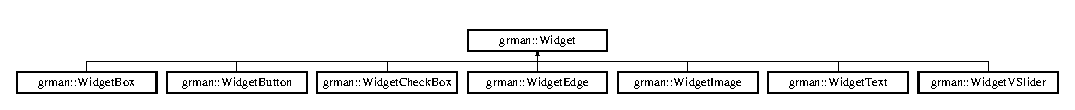
\includegraphics[height=1.025641cm]{classgrman_1_1_widget}
\end{center}
\end{figure}
\subsection*{Public Member Functions}
\begin{DoxyCompactItemize}
\item 
\mbox{\hyperlink{classgrman_1_1_widget_acaf342823ead0ea00f300f86c16f92c0}{Widget}} (double x, double y, double w, double h)
\begin{DoxyCompactList}\small\item\em Construction/\+Destruction. \end{DoxyCompactList}\item 
\mbox{\Hypertarget{classgrman_1_1_widget_acfd5cb20e83cb0cce4973530b467352b}\label{classgrman_1_1_widget_acfd5cb20e83cb0cce4973530b467352b}} 
\mbox{\hyperlink{classgrman_1_1_widget}{Widget}} $\ast$ \mbox{\hyperlink{classgrman_1_1_widget_acfd5cb20e83cb0cce4973530b467352b}{get\+\_\+child}} (int i)
\begin{DoxyCompactList}\small\item\em Gestion familiale... navigation et �dition de l\textquotesingle{}arbre des sous-\/�l�ments... \end{DoxyCompactList}\item 
\mbox{\Hypertarget{classgrman_1_1_widget_a35220289a92725ff9c7758f5c1f99580}\label{classgrman_1_1_widget_a35220289a92725ff9c7758f5c1f99580}} 
void {\bfseries add\+\_\+child} (\mbox{\hyperlink{classgrman_1_1_widget}{Widget}} \&elt)
\item 
\mbox{\Hypertarget{classgrman_1_1_widget_a6a67bda150ba51d4f53e165f336f4969}\label{classgrman_1_1_widget_a6a67bda150ba51d4f53e165f336f4969}} 
void {\bfseries remove\+\_\+child} (\mbox{\hyperlink{classgrman_1_1_widget}{Widget}} \&elt)
\item 
\mbox{\Hypertarget{classgrman_1_1_widget_a8251d948b6d2bfa5ebd61f9ae0b644a4}\label{classgrman_1_1_widget_a8251d948b6d2bfa5ebd61f9ae0b644a4}} 
void {\bfseries reframe} ()
\item 
\mbox{\Hypertarget{classgrman_1_1_widget_a61c632d3a7b2dee577e7a0be63fb16ff}\label{classgrman_1_1_widget_a61c632d3a7b2dee577e7a0be63fb16ff}} 
void \mbox{\hyperlink{classgrman_1_1_widget_a61c632d3a7b2dee577e7a0be63fb16ff}{set\+\_\+no\+\_\+gravity}} ()
\begin{DoxyCompactList}\small\item\em Gestion g�om�trie. \end{DoxyCompactList}\item 
\mbox{\Hypertarget{classgrman_1_1_widget_a0193f62e350fd481ccee016af8e5fada}\label{classgrman_1_1_widget_a0193f62e350fd481ccee016af8e5fada}} 
\mbox{\hyperlink{struct_frame}{Frame}} {\bfseries get\+\_\+abs\+\_\+frame} ()
\item 
\mbox{\Hypertarget{classgrman_1_1_widget_ac68b203c60fd2607f7bf92e01dfb80e8}\label{classgrman_1_1_widget_ac68b203c60fd2607f7bf92e01dfb80e8}} 
\mbox{\hyperlink{struct_coords}{Coords}} {\bfseries get\+\_\+abs\+\_\+pos} ()
\item 
\mbox{\Hypertarget{classgrman_1_1_widget_a634d670df3eb20c804565e77f08d578f}\label{classgrman_1_1_widget_a634d670df3eb20c804565e77f08d578f}} 
\mbox{\hyperlink{struct_coords}{Coords}} {\bfseries get\+\_\+center\+\_\+abs\+\_\+pos} ()
\item 
\mbox{\Hypertarget{classgrman_1_1_widget_aef604e011de42f7aebc667354855ef66}\label{classgrman_1_1_widget_aef604e011de42f7aebc667354855ef66}} 
void {\bfseries set\+\_\+frame} (\mbox{\hyperlink{struct_frame}{Frame}} frame)
\item 
\mbox{\Hypertarget{classgrman_1_1_widget_a5dacaf1ed4fc1c308e58ec4b364a378f}\label{classgrman_1_1_widget_a5dacaf1ed4fc1c308e58ec4b364a378f}} 
void {\bfseries set\+\_\+frame} (int x, int y, int w, int h)
\item 
\mbox{\Hypertarget{classgrman_1_1_widget_adadcb61c3bbbab13981ce7e070ef9844}\label{classgrman_1_1_widget_adadcb61c3bbbab13981ce7e070ef9844}} 
\mbox{\hyperlink{struct_frame}{Frame}} {\bfseries get\+\_\+frame} ()
\item 
\mbox{\Hypertarget{classgrman_1_1_widget_a5c304afbd87a913b5632c2941dde86d5}\label{classgrman_1_1_widget_a5c304afbd87a913b5632c2941dde86d5}} 
void {\bfseries set\+\_\+frame\+\_\+dim} (int w, int h)
\item 
\mbox{\Hypertarget{classgrman_1_1_widget_a3e4280294943b464185b826fc727fd47}\label{classgrman_1_1_widget_a3e4280294943b464185b826fc727fd47}} 
\mbox{\hyperlink{struct_coords}{Coords}} {\bfseries get\+\_\+frame\+\_\+dim} ()
\item 
\mbox{\Hypertarget{classgrman_1_1_widget_a7d1c6730f56dcb9445d1a554897fcdde}\label{classgrman_1_1_widget_a7d1c6730f56dcb9445d1a554897fcdde}} 
void {\bfseries set\+\_\+frame\+\_\+pos} (int x, int y)
\item 
\mbox{\Hypertarget{classgrman_1_1_widget_a829b46f419b8ad5ed932ec1b64007012}\label{classgrman_1_1_widget_a829b46f419b8ad5ed932ec1b64007012}} 
\mbox{\hyperlink{struct_coords}{Coords}} {\bfseries get\+\_\+frame\+\_\+pos} ()
\item 
\mbox{\Hypertarget{classgrman_1_1_widget_a5ae6e35c94712d55e44258bd5c4dee15}\label{classgrman_1_1_widget_a5ae6e35c94712d55e44258bd5c4dee15}} 
int {\bfseries get\+\_\+bp} ()
\item 
\mbox{\Hypertarget{classgrman_1_1_widget_a611f41523b29506c802ff341d81f11c5}\label{classgrman_1_1_widget_a611f41523b29506c802ff341d81f11c5}} 
int {\bfseries get\+\_\+parent\+\_\+bp} ()
\item 
\mbox{\Hypertarget{classgrman_1_1_widget_a7534b66cbf8327741a915e4d4f23b208}\label{classgrman_1_1_widget_a7534b66cbf8327741a915e4d4f23b208}} 
void {\bfseries set\+\_\+dimx} (int w)
\item 
\mbox{\Hypertarget{classgrman_1_1_widget_a50c994d9f3078f2b08ccd2dda6666595}\label{classgrman_1_1_widget_a50c994d9f3078f2b08ccd2dda6666595}} 
void {\bfseries set\+\_\+dimy} (int h)
\item 
\mbox{\Hypertarget{classgrman_1_1_widget_aefb181c21510565ba6ebdc1aedb716ad}\label{classgrman_1_1_widget_aefb181c21510565ba6ebdc1aedb716ad}} 
void {\bfseries set\+\_\+dim} (int w, int h)
\item 
\mbox{\Hypertarget{classgrman_1_1_widget_a8c8299f13852da3bece65c6a95750080}\label{classgrman_1_1_widget_a8c8299f13852da3bece65c6a95750080}} 
int {\bfseries get\+\_\+dimx} ()
\item 
\mbox{\Hypertarget{classgrman_1_1_widget_ab6471423114a8ddd56afacc2bde9f7e6}\label{classgrman_1_1_widget_ab6471423114a8ddd56afacc2bde9f7e6}} 
int {\bfseries get\+\_\+dimy} ()
\item 
\mbox{\Hypertarget{classgrman_1_1_widget_ae9d91c49ecc6458b43c850dbfe809f1a}\label{classgrman_1_1_widget_ae9d91c49ecc6458b43c850dbfe809f1a}} 
\mbox{\hyperlink{struct_coords}{Coords}} {\bfseries get\+\_\+dim} ()
\item 
\mbox{\Hypertarget{classgrman_1_1_widget_a8855590bf8b68f5e9e5e11084ed6f7da}\label{classgrman_1_1_widget_a8855590bf8b68f5e9e5e11084ed6f7da}} 
void {\bfseries set\+\_\+posx} (int x)
\item 
\mbox{\Hypertarget{classgrman_1_1_widget_a5655510a49e5f9f53ae41c55b5358c41}\label{classgrman_1_1_widget_a5655510a49e5f9f53ae41c55b5358c41}} 
void {\bfseries set\+\_\+posy} (int y)
\item 
\mbox{\Hypertarget{classgrman_1_1_widget_aa13b6833ffbec61374921c40be6f3188}\label{classgrman_1_1_widget_aa13b6833ffbec61374921c40be6f3188}} 
void {\bfseries set\+\_\+pos} (int x, int y)
\item 
\mbox{\Hypertarget{classgrman_1_1_widget_a2f806cd076f6e1924984f3556fa2e166}\label{classgrman_1_1_widget_a2f806cd076f6e1924984f3556fa2e166}} 
void {\bfseries set\+\_\+pos} (\mbox{\hyperlink{struct_coords}{Coords}} pos)
\item 
\mbox{\Hypertarget{classgrman_1_1_widget_ad1dd133abc3ffe41b05eea1485472285}\label{classgrman_1_1_widget_ad1dd133abc3ffe41b05eea1485472285}} 
int {\bfseries get\+\_\+posx} ()
\item 
\mbox{\Hypertarget{classgrman_1_1_widget_a3be06b9369e93dc60a19032547e90b0a}\label{classgrman_1_1_widget_a3be06b9369e93dc60a19032547e90b0a}} 
int {\bfseries get\+\_\+posy} ()
\item 
\mbox{\Hypertarget{classgrman_1_1_widget_a135a3118f755d970aacc093898f3afe3}\label{classgrman_1_1_widget_a135a3118f755d970aacc093898f3afe3}} 
\mbox{\hyperlink{struct_coords}{Coords}} {\bfseries get\+\_\+pos} ()
\item 
\mbox{\Hypertarget{classgrman_1_1_widget_a0be1eeef817874e6eb21571435a2eb76}\label{classgrman_1_1_widget_a0be1eeef817874e6eb21571435a2eb76}} 
void {\bfseries set\+\_\+gravity\+\_\+xy} (GravityX gx, GravityY gy)
\item 
\mbox{\Hypertarget{classgrman_1_1_widget_ac6b6d52a41f261f396f06320b7778e18}\label{classgrman_1_1_widget_ac6b6d52a41f261f396f06320b7778e18}} 
void {\bfseries set\+\_\+gravity\+\_\+x} (GravityX gx)
\item 
\mbox{\Hypertarget{classgrman_1_1_widget_a246c3dad41fd2b69b74d0924548398df}\label{classgrman_1_1_widget_a246c3dad41fd2b69b74d0924548398df}} 
void {\bfseries set\+\_\+gravity\+\_\+y} (GravityY gy)
\item 
\mbox{\Hypertarget{classgrman_1_1_widget_aea3772c724fd9ebd0a5c830439b0be4c}\label{classgrman_1_1_widget_aea3772c724fd9ebd0a5c830439b0be4c}} 
void {\bfseries set\+\_\+margin} (int margin)
\item 
\mbox{\Hypertarget{classgrman_1_1_widget_a1d96a55b2b8a61ec050e1dfa88a581c2}\label{classgrman_1_1_widget_a1d96a55b2b8a61ec050e1dfa88a581c2}} 
void {\bfseries set\+\_\+border} (int border)
\item 
\mbox{\Hypertarget{classgrman_1_1_widget_a5f1d6ebc1e01e380e34f6fda97c8b042}\label{classgrman_1_1_widget_a5f1d6ebc1e01e380e34f6fda97c8b042}} 
void {\bfseries set\+\_\+padding} (int padding)
\item 
\mbox{\Hypertarget{classgrman_1_1_widget_ae087f20809b9ec4ae1c0396d25aa7fb0}\label{classgrman_1_1_widget_ae087f20809b9ec4ae1c0396d25aa7fb0}} 
\mbox{\hyperlink{struct_frame}{Frame}} {\bfseries get\+\_\+parent\+\_\+frame} ()
\item 
\mbox{\Hypertarget{classgrman_1_1_widget_a4f4e9b1c845aee91bd8792100a4bcd8d}\label{classgrman_1_1_widget_a4f4e9b1c845aee91bd8792100a4bcd8d}} 
\mbox{\hyperlink{struct_frame}{Frame}} {\bfseries get\+\_\+parent\+\_\+abs\+\_\+frame} ()
\item 
\mbox{\Hypertarget{classgrman_1_1_widget_ac4c033333752a28ab9f345546f5c356e}\label{classgrman_1_1_widget_ac4c033333752a28ab9f345546f5c356e}} 
void {\bfseries reset\+\_\+posx} (int x)
\item 
\mbox{\Hypertarget{classgrman_1_1_widget_a27aa72773906212afb24de8524daee7a}\label{classgrman_1_1_widget_a27aa72773906212afb24de8524daee7a}} 
void {\bfseries reset\+\_\+posy} (int y)
\item 
\mbox{\Hypertarget{classgrman_1_1_widget_a22b2a25ad397e05dfd21fd834d667ec5}\label{classgrman_1_1_widget_a22b2a25ad397e05dfd21fd834d667ec5}} 
void \mbox{\hyperlink{classgrman_1_1_widget_a22b2a25ad397e05dfd21fd834d667ec5}{update}} ()
\begin{DoxyCompactList}\small\item\em Gestion affichage et interaction. \end{DoxyCompactList}\item 
void \mbox{\hyperlink{classgrman_1_1_widget_ab214adec555487fd72702eb735d445cc}{update\+\_\+interact}} ()
\begin{DoxyCompactList}\small\item\em Gestion des �v�nements. \end{DoxyCompactList}\item 
void \mbox{\hyperlink{classgrman_1_1_widget_afaee30b61971b479976f96eb8a9f7628}{update\+\_\+pre\+\_\+draw}} ()
\item 
void \mbox{\hyperlink{classgrman_1_1_widget_a581df4bb0e082d674253f142667a5d81}{update\+\_\+draw}} ()
\begin{DoxyCompactList}\small\item\em Gestion des affichages. \end{DoxyCompactList}\item 
\mbox{\Hypertarget{classgrman_1_1_widget_aad005761a6d7ac032a760df0872ab9c1}\label{classgrman_1_1_widget_aad005761a6d7ac032a760df0872ab9c1}} 
virtual void {\bfseries draw} ()
\item 
\mbox{\Hypertarget{classgrman_1_1_widget_a9020ab0e9f06cea13ff6553d4a157608}\label{classgrman_1_1_widget_a9020ab0e9f06cea13ff6553d4a157608}} 
virtual void {\bfseries draw\+\_\+border} ()
\item 
\mbox{\Hypertarget{classgrman_1_1_widget_a31929a6be1dfd317cd2b41afda8f1a6d}\label{classgrman_1_1_widget_a31929a6be1dfd317cd2b41afda8f1a6d}} 
virtual void {\bfseries interact\+\_\+over} ()
\item 
\mbox{\Hypertarget{classgrman_1_1_widget_a0e91fad56a2f62945bc151d951df9dd1}\label{classgrman_1_1_widget_a0e91fad56a2f62945bc151d951df9dd1}} 
virtual void {\bfseries interact\+\_\+focus} ()
\item 
\mbox{\Hypertarget{classgrman_1_1_widget_af6927f50345fedd1c2356c91490845b9}\label{classgrman_1_1_widget_af6927f50345fedd1c2356c91490845b9}} 
virtual void {\bfseries interact\+\_\+leave} ()
\item 
\mbox{\Hypertarget{classgrman_1_1_widget_a00c050eae20689d2d1420139916defdd}\label{classgrman_1_1_widget_a00c050eae20689d2d1420139916defdd}} 
virtual bool {\bfseries captures\+\_\+focus} ()
\item 
\mbox{\Hypertarget{classgrman_1_1_widget_a09e40491ed42e4804ed00718944209db}\label{classgrman_1_1_widget_a09e40491ed42e4804ed00718944209db}} 
bool {\bfseries is\+\_\+gui\+\_\+over} ()
\item 
\mbox{\Hypertarget{classgrman_1_1_widget_a2f37b348a6a7d91564ae3ab5fda91793}\label{classgrman_1_1_widget_a2f37b348a6a7d91564ae3ab5fda91793}} 
bool {\bfseries is\+\_\+gui\+\_\+focus} ()
\item 
\mbox{\Hypertarget{classgrman_1_1_widget_afb93db633b43f5003c3437bad3d7f9cf}\label{classgrman_1_1_widget_afb93db633b43f5003c3437bad3d7f9cf}} 
bool {\bfseries is\+\_\+gui\+\_\+leave} ()
\item 
\mbox{\Hypertarget{classgrman_1_1_widget_a7077b865ce348e339328aaaeb2fc4892}\label{classgrman_1_1_widget_a7077b865ce348e339328aaaeb2fc4892}} 
bool {\bfseries is\+\_\+mouse\+\_\+over} ()
\item 
\mbox{\Hypertarget{classgrman_1_1_widget_ae8f8fc19b6b0981895c38fdf7df4e4bb}\label{classgrman_1_1_widget_ae8f8fc19b6b0981895c38fdf7df4e4bb}} 
void \mbox{\hyperlink{classgrman_1_1_widget_ae8f8fc19b6b0981895c38fdf7df4e4bb}{set\+\_\+bg\+\_\+color}} (int bgc)
\begin{DoxyCompactList}\small\item\em Les accesseurs de \char`\"{}styles\char`\"{} sont � compl�ter... \end{DoxyCompactList}\item 
\mbox{\Hypertarget{classgrman_1_1_widget_a53be51006d3635bfbcf6780df1237536}\label{classgrman_1_1_widget_a53be51006d3635bfbcf6780df1237536}} 
int {\bfseries get\+\_\+border\+\_\+color} ()
\item 
\mbox{\Hypertarget{classgrman_1_1_widget_aa906e75b8fcd1fdc753161f64718b404}\label{classgrman_1_1_widget_aa906e75b8fcd1fdc753161f64718b404}} 
{\bfseries Widget} (const \mbox{\hyperlink{classgrman_1_1_widget}{Widget}} \&)=delete
\item 
\mbox{\Hypertarget{classgrman_1_1_widget_a6107b4213ddcf3c75bab9cb383d69285}\label{classgrman_1_1_widget_a6107b4213ddcf3c75bab9cb383d69285}} 
\mbox{\hyperlink{classgrman_1_1_widget}{Widget}} \& {\bfseries operator=} (const \mbox{\hyperlink{classgrman_1_1_widget}{Widget}} \&)=delete
\end{DoxyCompactItemize}
\subsection*{Protected Attributes}
\begin{DoxyCompactItemize}
\item 
\mbox{\Hypertarget{classgrman_1_1_widget_af3f27be4d61ce1d2376148ada839a622}\label{classgrman_1_1_widget_af3f27be4d61ce1d2376148ada839a622}} 
\mbox{\hyperlink{classgrman_1_1_widget}{Widget}} $\ast$ {\bfseries m\+\_\+parent} = nullptr
\item 
\mbox{\Hypertarget{classgrman_1_1_widget_adaf4dd515f19c5c1c461ef39a8980c11}\label{classgrman_1_1_widget_adaf4dd515f19c5c1c461ef39a8980c11}} 
std\+::vector$<$ \mbox{\hyperlink{classgrman_1_1_widget}{Widget}} $\ast$ $>$ \mbox{\hyperlink{classgrman_1_1_widget_adaf4dd515f19c5c1c461ef39a8980c11}{m\+\_\+children}}
\begin{DoxyCompactList}\small\item\em Naked pointers \+: Dangerous... \end{DoxyCompactList}\item 
\mbox{\Hypertarget{classgrman_1_1_widget_a8dd9b7ffb53fed222b4db4d5d82c6a85}\label{classgrman_1_1_widget_a8dd9b7ffb53fed222b4db4d5d82c6a85}} 
\mbox{\hyperlink{struct_frame}{Frame}} {\bfseries m\+\_\+frame}
\item 
\mbox{\Hypertarget{classgrman_1_1_widget_ae7b67ea60ac8bc619210d1b13a9ef402}\label{classgrman_1_1_widget_ae7b67ea60ac8bc619210d1b13a9ef402}} 
\mbox{\hyperlink{struct_frame}{Frame}} {\bfseries m\+\_\+abs\+\_\+frame}
\item 
\mbox{\Hypertarget{classgrman_1_1_widget_a355f414f0b961981e798f50e832ea23f}\label{classgrman_1_1_widget_a355f414f0b961981e798f50e832ea23f}} 
B\+I\+T\+M\+AP $\ast$ {\bfseries m\+\_\+view} = nullptr
\item 
\mbox{\Hypertarget{classgrman_1_1_widget_a3cc7ad80745c4258cf86d1b0c61f279c}\label{classgrman_1_1_widget_a3cc7ad80745c4258cf86d1b0c61f279c}} 
B\+I\+T\+M\+AP $\ast$ {\bfseries m\+\_\+view\+\_\+wb} = nullptr
\item 
\mbox{\Hypertarget{classgrman_1_1_widget_a6ea6c3805aab95fedc967829357ca182}\label{classgrman_1_1_widget_a6ea6c3805aab95fedc967829357ca182}} 
GravityX {\bfseries m\+\_\+gravity\+\_\+x} = Gravity\+X\+::\+Center
\item 
\mbox{\Hypertarget{classgrman_1_1_widget_a626ab06181897a675409c7a927256330}\label{classgrman_1_1_widget_a626ab06181897a675409c7a927256330}} 
GravityY {\bfseries m\+\_\+gravity\+\_\+y} = Gravity\+Y\+::\+Center
\item 
\mbox{\Hypertarget{classgrman_1_1_widget_ab4c5ea6ee9fe629a7bba08c296d4f9d1}\label{classgrman_1_1_widget_ab4c5ea6ee9fe629a7bba08c296d4f9d1}} 
int {\bfseries m\+\_\+bg\+\_\+color} = -\/1
\item 
\mbox{\Hypertarget{classgrman_1_1_widget_af55f7f94d96c8c7b18853b3a6d969bb0}\label{classgrman_1_1_widget_af55f7f94d96c8c7b18853b3a6d969bb0}} 
int {\bfseries m\+\_\+border\+\_\+color} = G\+R\+I\+S\+S\+O\+M\+B\+RE
\item 
\mbox{\Hypertarget{classgrman_1_1_widget_ab3daa933fcfcc7906ec578f95a33bc2c}\label{classgrman_1_1_widget_ab3daa933fcfcc7906ec578f95a33bc2c}} 
int {\bfseries m\+\_\+border\+\_\+color\+\_\+over} = V\+I\+O\+L\+E\+T\+S\+O\+M\+B\+RE
\item 
\mbox{\Hypertarget{classgrman_1_1_widget_ab8e92c292a2ad1de692846b1c2dca12d}\label{classgrman_1_1_widget_ab8e92c292a2ad1de692846b1c2dca12d}} 
int {\bfseries m\+\_\+border\+\_\+color\+\_\+focus} = O\+R\+A\+N\+G\+E\+S\+O\+M\+B\+RE
\item 
\mbox{\Hypertarget{classgrman_1_1_widget_a817f5bee11166fa0e0caeb9deef0c2d3}\label{classgrman_1_1_widget_a817f5bee11166fa0e0caeb9deef0c2d3}} 
int {\bfseries m\+\_\+border} = 1
\item 
\mbox{\Hypertarget{classgrman_1_1_widget_a2587bb6d21b32a0b8921b099e6e917bb}\label{classgrman_1_1_widget_a2587bb6d21b32a0b8921b099e6e917bb}} 
int {\bfseries m\+\_\+margin} = 1
\item 
\mbox{\Hypertarget{classgrman_1_1_widget_a130216f6cc51b9fdd3d9724eaa14f026}\label{classgrman_1_1_widget_a130216f6cc51b9fdd3d9724eaa14f026}} 
int {\bfseries m\+\_\+padding} = 1
\end{DoxyCompactItemize}


\subsection{Detailed Description}
Cette classe est trop grosse, elle fait le repassage, r�pare la voiture, p�che au harpon... En principe il faut revoir la conception quand une classe devient aussi grosse (refactoriser) Par exemple une classe de base \mbox{\hyperlink{classgrman_1_1_widget}{Widget}} pour l\textquotesingle{}aspect composite et une classe d�riv�e Widget\+Decorated pour les styles 

Definition at line 43 of file widget.\+h.



\subsection{Constructor \& Destructor Documentation}
\mbox{\Hypertarget{classgrman_1_1_widget_acaf342823ead0ea00f300f86c16f92c0}\label{classgrman_1_1_widget_acaf342823ead0ea00f300f86c16f92c0}} 
\index{grman\+::\+Widget@{grman\+::\+Widget}!Widget@{Widget}}
\index{Widget@{Widget}!grman\+::\+Widget@{grman\+::\+Widget}}
\subsubsection{\texorpdfstring{Widget()}{Widget()}}
{\footnotesize\ttfamily grman\+::\+Widget\+::\+Widget (\begin{DoxyParamCaption}\item[{double}]{x,  }\item[{double}]{y,  }\item[{double}]{w,  }\item[{double}]{h }\end{DoxyParamCaption})\hspace{0.3cm}{\ttfamily [inline]}}



Construction/\+Destruction. 

M�thodes utilisables dans les classes d�riv�es et les classes qui ont un \mbox{\hyperlink{classgrman_1_1_widget}{Widget}} ou d�riv� en attribut 

Definition at line 77 of file widget.\+h.



\subsection{Member Function Documentation}
\mbox{\Hypertarget{classgrman_1_1_widget_a581df4bb0e082d674253f142667a5d81}\label{classgrman_1_1_widget_a581df4bb0e082d674253f142667a5d81}} 
\index{grman\+::\+Widget@{grman\+::\+Widget}!update\+\_\+draw@{update\+\_\+draw}}
\index{update\+\_\+draw@{update\+\_\+draw}!grman\+::\+Widget@{grman\+::\+Widget}}
\subsubsection{\texorpdfstring{update\+\_\+draw()}{update\_draw()}}
{\footnotesize\ttfamily void grman\+::\+Widget\+::update\+\_\+draw (\begin{DoxyParamCaption}{ }\end{DoxyParamCaption})}



Gestion des affichages. 

Propagation de l\textquotesingle{}update aux elements enfants On affiche en dernier (devant les autres) les �l�ments ajout�s en dernier 

Definition at line 69 of file widget.\+cpp.

\mbox{\Hypertarget{classgrman_1_1_widget_ab214adec555487fd72702eb735d445cc}\label{classgrman_1_1_widget_ab214adec555487fd72702eb735d445cc}} 
\index{grman\+::\+Widget@{grman\+::\+Widget}!update\+\_\+interact@{update\+\_\+interact}}
\index{update\+\_\+interact@{update\+\_\+interact}!grman\+::\+Widget@{grman\+::\+Widget}}
\subsubsection{\texorpdfstring{update\+\_\+interact()}{update\_interact()}}
{\footnotesize\ttfamily void grman\+::\+Widget\+::update\+\_\+interact (\begin{DoxyParamCaption}{ }\end{DoxyParamCaption})}



Gestion des �v�nements. 

Propagation de l\textquotesingle{}update aux elements enfants On interagit en 1er avec les �l�ments ajout�s en dernier 

Definition at line 27 of file widget.\+cpp.

\mbox{\Hypertarget{classgrman_1_1_widget_afaee30b61971b479976f96eb8a9f7628}\label{classgrman_1_1_widget_afaee30b61971b479976f96eb8a9f7628}} 
\index{grman\+::\+Widget@{grman\+::\+Widget}!update\+\_\+pre\+\_\+draw@{update\+\_\+pre\+\_\+draw}}
\index{update\+\_\+pre\+\_\+draw@{update\+\_\+pre\+\_\+draw}!grman\+::\+Widget@{grman\+::\+Widget}}
\subsubsection{\texorpdfstring{update\+\_\+pre\+\_\+draw()}{update\_pre\_draw()}}
{\footnotesize\ttfamily void grman\+::\+Widget\+::update\+\_\+pre\+\_\+draw (\begin{DoxyParamCaption}{ }\end{DoxyParamCaption})}

Gestion des affichages, 1�re passe pour fixer les cadres (N�cessaire pour les liens \+: affich�s au fond donc en 1er mais s\textquotesingle{}appuyant sur les positions des autres qui sont affich�s apr�s) Propagation de l\textquotesingle{}update aux elements enfants 

Definition at line 56 of file widget.\+cpp.



The documentation for this class was generated from the following files\+:\begin{DoxyCompactItemize}
\item 
grman/widget.\+h\item 
grman/widget.\+cpp\end{DoxyCompactItemize}

\hypertarget{classgrman_1_1_widget_box}{}\section{grman\+:\+:Widget\+Box Class Reference}
\label{classgrman_1_1_widget_box}\index{grman\+::\+Widget\+Box@{grman\+::\+Widget\+Box}}
Inheritance diagram for grman\+:\+:Widget\+Box\+:\begin{figure}[H]
\begin{center}
\leavevmode
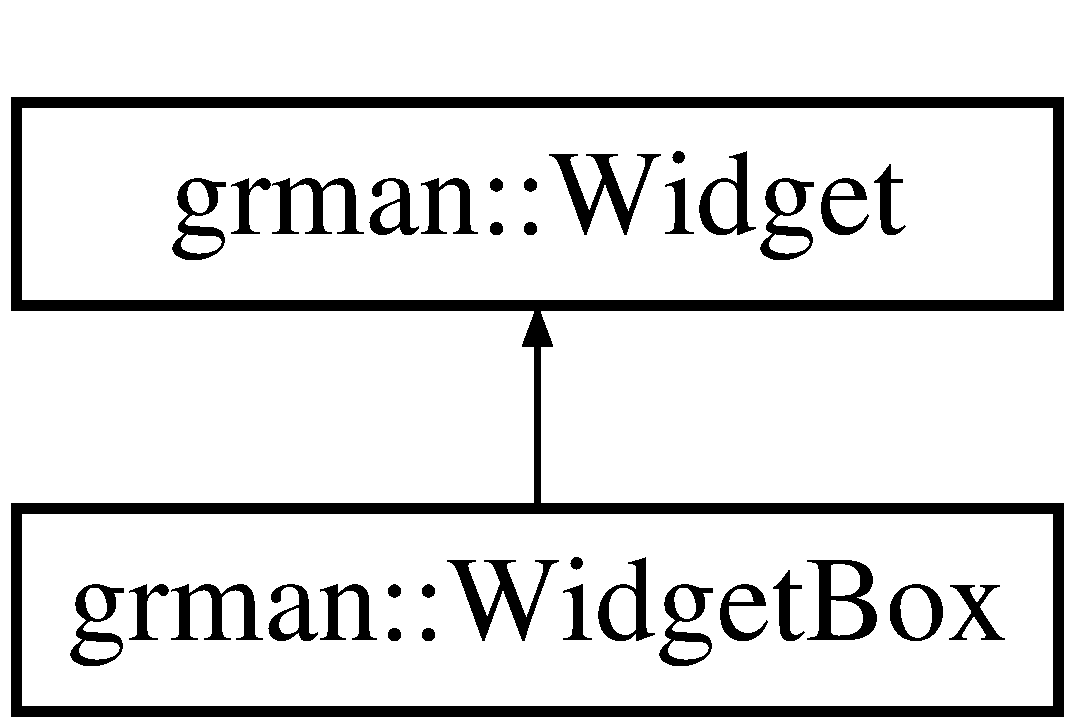
\includegraphics[height=2.000000cm]{classgrman_1_1_widget_box}
\end{center}
\end{figure}
\subsection*{Public Member Functions}
\begin{DoxyCompactItemize}
\item 
\mbox{\Hypertarget{classgrman_1_1_widget_box_a5de9d1bfbe85e470cdcc6ebb00f36b26}\label{classgrman_1_1_widget_box_a5de9d1bfbe85e470cdcc6ebb00f36b26}} 
virtual void {\bfseries interact\+\_\+focus} ()
\item 
\mbox{\Hypertarget{classgrman_1_1_widget_box_a2f9311b8df4e9add38fd595e0eaf2ec9}\label{classgrman_1_1_widget_box_a2f9311b8df4e9add38fd595e0eaf2ec9}} 
virtual bool {\bfseries captures\+\_\+focus} ()
\item 
\mbox{\Hypertarget{classgrman_1_1_widget_box_a96f1aa069e1271d48e10ca91a6928ee9}\label{classgrman_1_1_widget_box_a96f1aa069e1271d48e10ca91a6928ee9}} 
void {\bfseries set\+\_\+moveable} (bool moveable=true)
\end{DoxyCompactItemize}
\subsection*{Protected Attributes}
\begin{DoxyCompactItemize}
\item 
\mbox{\Hypertarget{classgrman_1_1_widget_box_a5db31005a4eaa084416ff9d1a2fd738d}\label{classgrman_1_1_widget_box_a5db31005a4eaa084416ff9d1a2fd738d}} 
bool {\bfseries m\+\_\+moveable} = false
\item 
\mbox{\Hypertarget{classgrman_1_1_widget_box_ae8758f26d89a067827321bbd0bfb43fc}\label{classgrman_1_1_widget_box_ae8758f26d89a067827321bbd0bfb43fc}} 
bool {\bfseries m\+\_\+contained} = true
\item 
\mbox{\Hypertarget{classgrman_1_1_widget_box_aed748b443a9737dc7cdef6022ae53950}\label{classgrman_1_1_widget_box_aed748b443a9737dc7cdef6022ae53950}} 
\mbox{\hyperlink{struct_coords}{Coords}} {\bfseries m\+\_\+pos\+\_\+start\+\_\+move}
\end{DoxyCompactItemize}


\subsection{Detailed Description}


Definition at line 349 of file widget.\+h.



The documentation for this class was generated from the following files\+:\begin{DoxyCompactItemize}
\item 
grman/widget.\+h\item 
grman/widget.\+cpp\end{DoxyCompactItemize}

\hypertarget{classgrman_1_1_widget_button}{}\section{grman\+:\+:Widget\+Button Class Reference}
\label{classgrman_1_1_widget_button}\index{grman\+::\+Widget\+Button@{grman\+::\+Widget\+Button}}
Inheritance diagram for grman\+:\+:Widget\+Button\+:\begin{figure}[H]
\begin{center}
\leavevmode
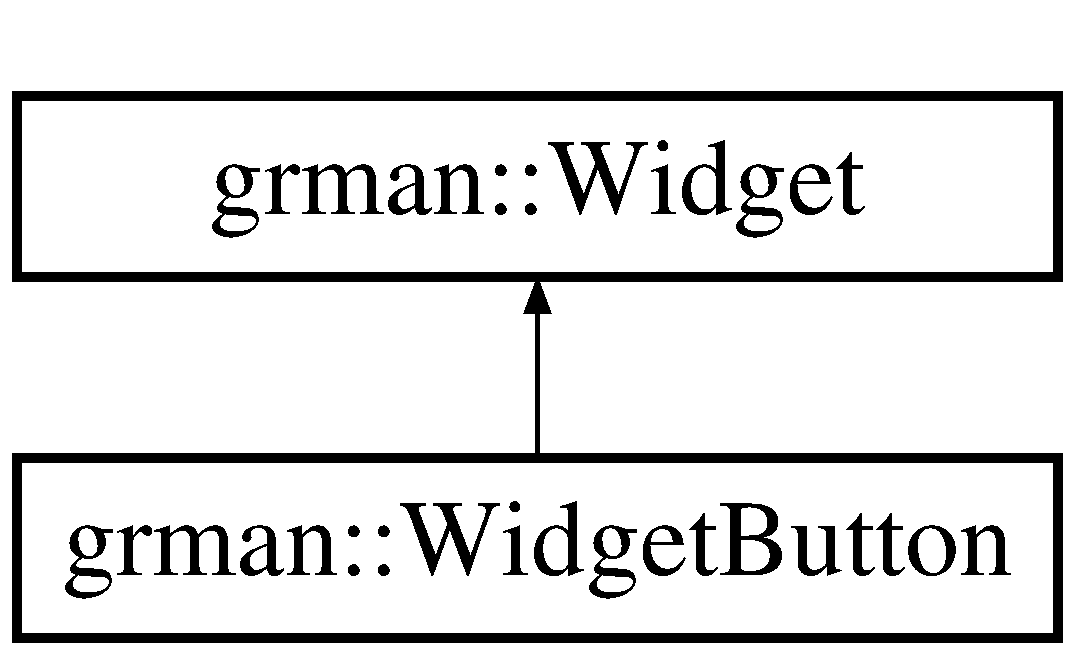
\includegraphics[height=2.000000cm]{classgrman_1_1_widget_button}
\end{center}
\end{figure}
\subsection*{Public Member Functions}
\begin{DoxyCompactItemize}
\item 
\mbox{\Hypertarget{classgrman_1_1_widget_button_aba1ce188474cc3c0feea1ae5a8d28117}\label{classgrman_1_1_widget_button_aba1ce188474cc3c0feea1ae5a8d28117}} 
virtual void {\bfseries interact\+\_\+focus} ()
\item 
\mbox{\Hypertarget{classgrman_1_1_widget_button_a11e2dbaa31e7b1787c69281564a5d248}\label{classgrman_1_1_widget_button_a11e2dbaa31e7b1787c69281564a5d248}} 
virtual bool {\bfseries captures\+\_\+focus} ()
\item 
\mbox{\Hypertarget{classgrman_1_1_widget_button_a3460c3ffbad5cee3de9b58c032300b84}\label{classgrman_1_1_widget_button_a3460c3ffbad5cee3de9b58c032300b84}} 
bool {\bfseries clicked} ()
\item 
\mbox{\Hypertarget{classgrman_1_1_widget_button_a66f18e14fc5d97f2c3f2af0c65420770}\label{classgrman_1_1_widget_button_a66f18e14fc5d97f2c3f2af0c65420770}} 
bool {\bfseries get\+\_\+value} ()
\item 
\mbox{\Hypertarget{classgrman_1_1_widget_button_a2238b547dfb79663c9a3555aa06f87f3}\label{classgrman_1_1_widget_button_a2238b547dfb79663c9a3555aa06f87f3}} 
void {\bfseries set\+\_\+value} (bool value)
\end{DoxyCompactItemize}
\subsection*{Protected Attributes}
\begin{DoxyCompactItemize}
\item 
\mbox{\Hypertarget{classgrman_1_1_widget_button_a08dc2cd729c616d855dd3b226ee8082a}\label{classgrman_1_1_widget_button_a08dc2cd729c616d855dd3b226ee8082a}} 
bool {\bfseries m\+\_\+value} = false
\end{DoxyCompactItemize}


\subsection{Detailed Description}


Definition at line 257 of file widget.\+h.



The documentation for this class was generated from the following files\+:\begin{DoxyCompactItemize}
\item 
grman/widget.\+h\item 
grman/widget.\+cpp\end{DoxyCompactItemize}

\hypertarget{classgrman_1_1_widget_check_box}{}\section{grman\+:\+:Widget\+Check\+Box Class Reference}
\label{classgrman_1_1_widget_check_box}\index{grman\+::\+Widget\+Check\+Box@{grman\+::\+Widget\+Check\+Box}}
Inheritance diagram for grman\+:\+:Widget\+Check\+Box\+:\begin{figure}[H]
\begin{center}
\leavevmode
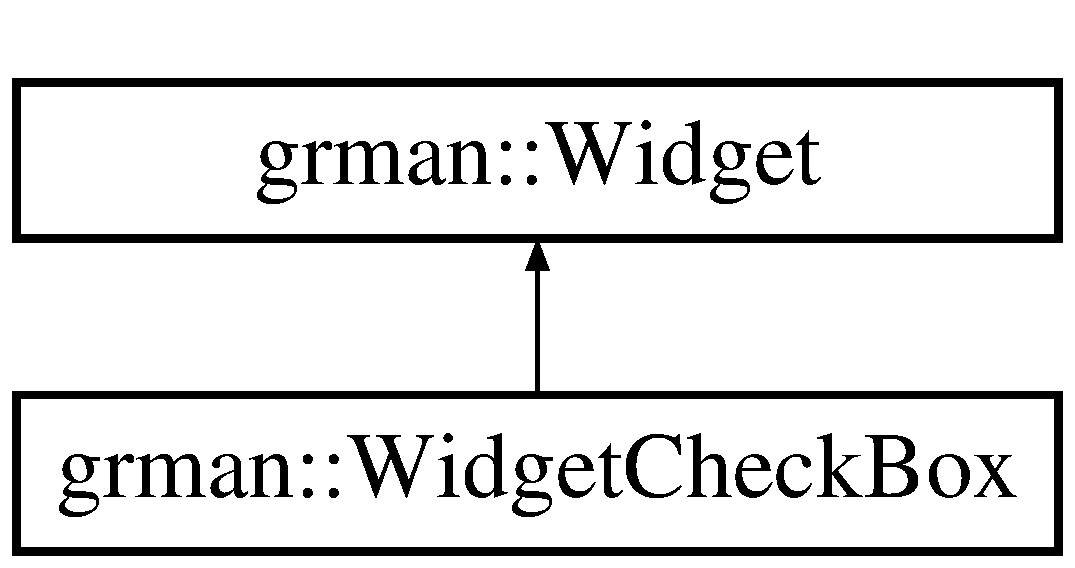
\includegraphics[height=2.000000cm]{classgrman_1_1_widget_check_box}
\end{center}
\end{figure}
\subsection*{Public Member Functions}
\begin{DoxyCompactItemize}
\item 
\mbox{\Hypertarget{classgrman_1_1_widget_check_box_af935c38c495fb97868712b0eefe6a314}\label{classgrman_1_1_widget_check_box_af935c38c495fb97868712b0eefe6a314}} 
virtual void {\bfseries draw} ()
\item 
\mbox{\Hypertarget{classgrman_1_1_widget_check_box_a14adf9ff412d2fa9ce5c52cbe4322945}\label{classgrman_1_1_widget_check_box_a14adf9ff412d2fa9ce5c52cbe4322945}} 
virtual void {\bfseries interact\+\_\+focus} ()
\item 
\mbox{\Hypertarget{classgrman_1_1_widget_check_box_a5b87e7f1073c4a189dff42d18db3c87f}\label{classgrman_1_1_widget_check_box_a5b87e7f1073c4a189dff42d18db3c87f}} 
virtual bool {\bfseries captures\+\_\+focus} ()
\item 
\mbox{\Hypertarget{classgrman_1_1_widget_check_box_ab591b2df3943adde9318dd6db25ca845}\label{classgrman_1_1_widget_check_box_ab591b2df3943adde9318dd6db25ca845}} 
bool {\bfseries get\+\_\+value} ()
\item 
\mbox{\Hypertarget{classgrman_1_1_widget_check_box_ad5236c112a398d2d2c17360dc4f76f4b}\label{classgrman_1_1_widget_check_box_ad5236c112a398d2d2c17360dc4f76f4b}} 
void {\bfseries set\+\_\+value} (bool value)
\end{DoxyCompactItemize}
\subsection*{Protected Attributes}
\begin{DoxyCompactItemize}
\item 
\mbox{\Hypertarget{classgrman_1_1_widget_check_box_ae430ada493e002e9c91b458f3ffa9678}\label{classgrman_1_1_widget_check_box_ae430ada493e002e9c91b458f3ffa9678}} 
bool {\bfseries m\+\_\+value} = false
\end{DoxyCompactItemize}


\subsection{Detailed Description}


Definition at line 236 of file widget.\+h.



The documentation for this class was generated from the following files\+:\begin{DoxyCompactItemize}
\item 
grman/widget.\+h\item 
grman/widget.\+cpp\end{DoxyCompactItemize}

\hypertarget{classgrman_1_1_widget_edge}{}\section{grman\+:\+:Widget\+Edge Class Reference}
\label{classgrman_1_1_widget_edge}\index{grman\+::\+Widget\+Edge@{grman\+::\+Widget\+Edge}}
Inheritance diagram for grman\+:\+:Widget\+Edge\+:\begin{figure}[H]
\begin{center}
\leavevmode
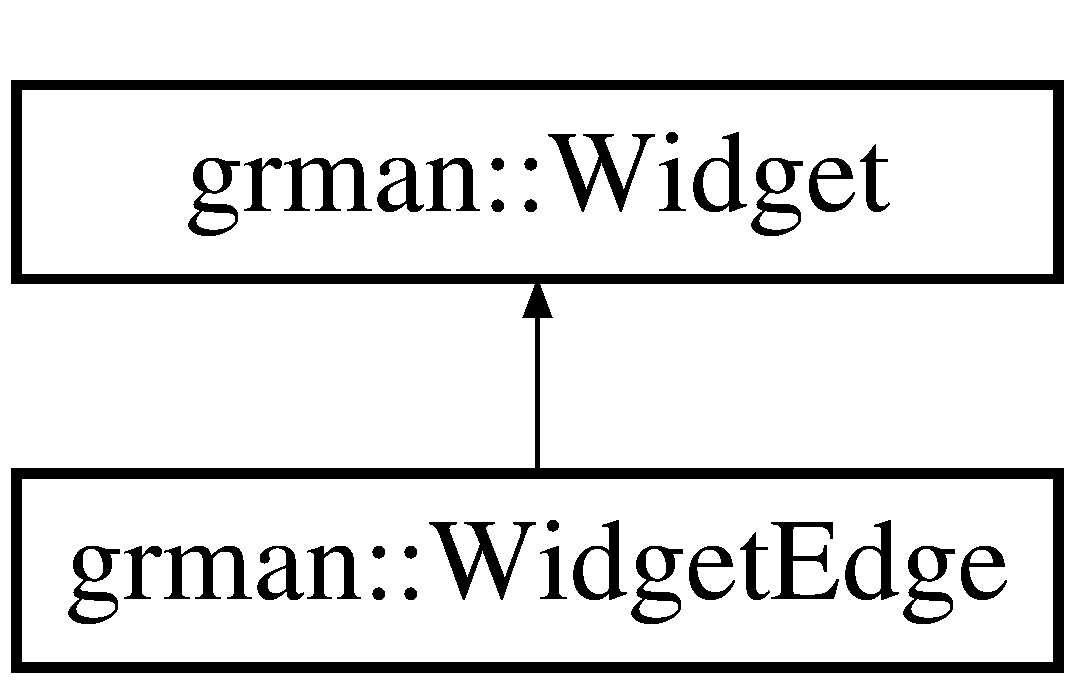
\includegraphics[height=2.000000cm]{classgrman_1_1_widget_edge}
\end{center}
\end{figure}
\subsection*{Public Member Functions}
\begin{DoxyCompactItemize}
\item 
virtual void \mbox{\hyperlink{classgrman_1_1_widget_edge_adbaeb94bef0a5334fd3ddc0fe30343c5}{draw}} ()
\item 
\mbox{\Hypertarget{classgrman_1_1_widget_edge_ad28a27ac45fe76a43e56c4fc97f57d89}\label{classgrman_1_1_widget_edge_ad28a27ac45fe76a43e56c4fc97f57d89}} 
void {\bfseries attach\+\_\+from} (\mbox{\hyperlink{classgrman_1_1_widget}{Widget}} \&from)
\item 
\mbox{\Hypertarget{classgrman_1_1_widget_edge_a82240d34e4e099b935e410dfe9b031cf}\label{classgrman_1_1_widget_edge_a82240d34e4e099b935e410dfe9b031cf}} 
void {\bfseries attach\+\_\+to} (\mbox{\hyperlink{classgrman_1_1_widget}{Widget}} \&to)
\item 
\mbox{\Hypertarget{classgrman_1_1_widget_edge_afe5f45cb7b4b36f01ff52538df0891e4}\label{classgrman_1_1_widget_edge_afe5f45cb7b4b36f01ff52538df0891e4}} 
void {\bfseries reset\+\_\+no\+\_\+items} ()
\item 
\mbox{\Hypertarget{classgrman_1_1_widget_edge_afbe9483635cc9d3bf934f154a36c5936}\label{classgrman_1_1_widget_edge_afbe9483635cc9d3bf934f154a36c5936}} 
void {\bfseries reset\+\_\+arrow} ()
\item 
\mbox{\Hypertarget{classgrman_1_1_widget_edge_af509a89d939f07c3db1a2ad47f69f760}\label{classgrman_1_1_widget_edge_af509a89d939f07c3db1a2ad47f69f760}} 
void {\bfseries reset\+\_\+arrow\+\_\+with\+\_\+bullet} ()
\item 
\mbox{\Hypertarget{classgrman_1_1_widget_edge_a28984f345cdebfd03833b69dbfe079e6}\label{classgrman_1_1_widget_edge_a28984f345cdebfd03833b69dbfe079e6}} 
void {\bfseries reset\+\_\+middle\+\_\+arrow} ()
\item 
\mbox{\Hypertarget{classgrman_1_1_widget_edge_a7dd45ab136a5bde2f75b93fcfaaab281}\label{classgrman_1_1_widget_edge_a7dd45ab136a5bde2f75b93fcfaaab281}} 
void {\bfseries reset\+\_\+middle\+\_\+arrow\+\_\+with\+\_\+bullets} ()
\item 
\mbox{\Hypertarget{classgrman_1_1_widget_edge_a86413db4c60fd85d249667b55f8d4d1a}\label{classgrman_1_1_widget_edge_a86413db4c60fd85d249667b55f8d4d1a}} 
void {\bfseries add\+\_\+item} (\mbox{\hyperlink{structgrman_1_1_arrow_item}{Arrow\+Item}} ai)
\item 
\mbox{\Hypertarget{classgrman_1_1_widget_edge_ab8e0a11fb4d0a465aea36736e683c76d}\label{classgrman_1_1_widget_edge_ab8e0a11fb4d0a465aea36736e683c76d}} 
void {\bfseries set\+\_\+children\+\_\+position} (double rel\+\_\+pos)
\item 
\mbox{\Hypertarget{classgrman_1_1_widget_edge_abb666eb206a3777171883ef638708c74}\label{classgrman_1_1_widget_edge_abb666eb206a3777171883ef638708c74}} 
void {\bfseries set\+\_\+children\+\_\+lateral} (double abs\+\_\+lat)
\end{DoxyCompactItemize}
\subsection*{Protected Attributes}
\begin{DoxyCompactItemize}
\item 
\mbox{\hyperlink{classgrman_1_1_widget}{Widget}} $\ast$ \mbox{\hyperlink{classgrman_1_1_widget_edge_ac80f872a3c762175fb8067728faee007}{m\+\_\+attach}} \mbox{[}2\mbox{]} = \{nullptr, nullptr\}
\item 
\mbox{\Hypertarget{classgrman_1_1_widget_edge_acc06b753b4d1898226a1d6b256db541e}\label{classgrman_1_1_widget_edge_acc06b753b4d1898226a1d6b256db541e}} 
std\+::vector$<$ \mbox{\hyperlink{structgrman_1_1_arrow_item}{Arrow\+Item}} $>$ {\bfseries m\+\_\+items}
\item 
\mbox{\Hypertarget{classgrman_1_1_widget_edge_a07ba980c6b3aba81d150c823a33e1642}\label{classgrman_1_1_widget_edge_a07ba980c6b3aba81d150c823a33e1642}} 
int {\bfseries m\+\_\+color} = G\+R\+I\+S\+S\+O\+M\+B\+RE
\item 
\mbox{\Hypertarget{classgrman_1_1_widget_edge_ae03251d33cb4879a90e23726aa7eb280}\label{classgrman_1_1_widget_edge_ae03251d33cb4879a90e23726aa7eb280}} 
int {\bfseries m\+\_\+thickness} = 2
\item 
\mbox{\Hypertarget{classgrman_1_1_widget_edge_a83b0c644beee05cd3a36ffe2f9675d04}\label{classgrman_1_1_widget_edge_a83b0c644beee05cd3a36ffe2f9675d04}} 
double {\bfseries m\+\_\+children\+\_\+position} = 0.\+5
\item 
\mbox{\Hypertarget{classgrman_1_1_widget_edge_a67aa0a57bece3e2f6c59216984567a38}\label{classgrman_1_1_widget_edge_a67aa0a57bece3e2f6c59216984567a38}} 
double {\bfseries m\+\_\+children\+\_\+lateral} = 16
\end{DoxyCompactItemize}


\subsection{Detailed Description}


Definition at line 402 of file widget.\+h.



\subsection{Member Function Documentation}
\mbox{\Hypertarget{classgrman_1_1_widget_edge_adbaeb94bef0a5334fd3ddc0fe30343c5}\label{classgrman_1_1_widget_edge_adbaeb94bef0a5334fd3ddc0fe30343c5}} 
\index{grman\+::\+Widget\+Edge@{grman\+::\+Widget\+Edge}!draw@{draw}}
\index{draw@{draw}!grman\+::\+Widget\+Edge@{grman\+::\+Widget\+Edge}}
\subsubsection{\texorpdfstring{draw()}{draw()}}
{\footnotesize\ttfamily void grman\+::\+Widget\+Edge\+::draw (\begin{DoxyParamCaption}{ }\end{DoxyParamCaption})\hspace{0.3cm}{\ttfamily [virtual]}}

La suite concerne les �l�ments de d�corations, fl�ches/extr�mit�s Pour chaque �l�ment de d�coration du lien... ~\newline
~\newline
~\newline
~\newline
 Cas Bullet

Cas pointe de fl�che ou triangle

Pointe de fl�che

Triangle 

Reimplemented from \mbox{\hyperlink{classgrman_1_1_widget}{grman\+::\+Widget}}.



Definition at line 344 of file widget.\+cpp.



\subsection{Member Data Documentation}
\mbox{\Hypertarget{classgrman_1_1_widget_edge_ac80f872a3c762175fb8067728faee007}\label{classgrman_1_1_widget_edge_ac80f872a3c762175fb8067728faee007}} 
\index{grman\+::\+Widget\+Edge@{grman\+::\+Widget\+Edge}!m\+\_\+attach@{m\+\_\+attach}}
\index{m\+\_\+attach@{m\+\_\+attach}!grman\+::\+Widget\+Edge@{grman\+::\+Widget\+Edge}}
\subsubsection{\texorpdfstring{m\+\_\+attach}{m\_attach}}
{\footnotesize\ttfamily \mbox{\hyperlink{classgrman_1_1_widget}{Widget}}$\ast$ grman\+::\+Widget\+Edge\+::m\+\_\+attach\mbox{[}2\mbox{]} = \{nullptr, nullptr\}\hspace{0.3cm}{\ttfamily [protected]}}

Si un de 2 pointeur est � nul, l\textquotesingle{}ar�te n\textquotesingle{}est pas trait�e Si les 2 pointeurs sont distincts du nul l\textquotesingle{}ar�te est trait� Les 2 instances point�es ne doivent pas �tre d�truites sous peine de plantage douloureux du programme ! 

Definition at line 411 of file widget.\+h.



The documentation for this class was generated from the following files\+:\begin{DoxyCompactItemize}
\item 
grman/widget.\+h\item 
grman/widget.\+cpp\end{DoxyCompactItemize}

\hypertarget{classgrman_1_1_widget_image}{}\section{grman\+:\+:Widget\+Image Class Reference}
\label{classgrman_1_1_widget_image}\index{grman\+::\+Widget\+Image@{grman\+::\+Widget\+Image}}
Inheritance diagram for grman\+:\+:Widget\+Image\+:\begin{figure}[H]
\begin{center}
\leavevmode
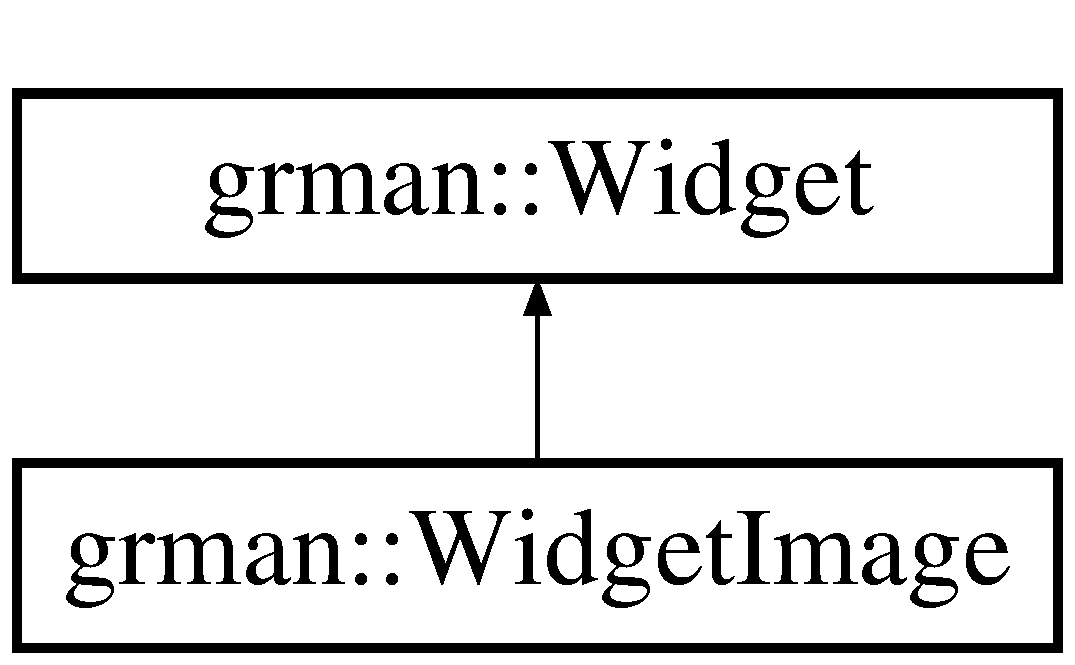
\includegraphics[height=2.000000cm]{classgrman_1_1_widget_image}
\end{center}
\end{figure}
\subsection*{Public Member Functions}
\begin{DoxyCompactItemize}
\item 
\mbox{\Hypertarget{classgrman_1_1_widget_image_af9a67025da24eeea3d3ebcea0f492ed1}\label{classgrman_1_1_widget_image_af9a67025da24eeea3d3ebcea0f492ed1}} 
{\bfseries Widget\+Image} (std\+::string pic\+\_\+name=\char`\"{}\char`\"{})
\item 
\mbox{\Hypertarget{classgrman_1_1_widget_image_a06e44ca3302524a1ec5c7eacf16ca2b3}\label{classgrman_1_1_widget_image_a06e44ca3302524a1ec5c7eacf16ca2b3}} 
virtual void {\bfseries draw} ()
\item 
\mbox{\Hypertarget{classgrman_1_1_widget_image_af164b59bc1533a8215f438c84f891c2a}\label{classgrman_1_1_widget_image_af164b59bc1533a8215f438c84f891c2a}} 
virtual void {\bfseries reframe} ()
\item 
\mbox{\Hypertarget{classgrman_1_1_widget_image_a024e6d7101993d1dbc022f02241e3484}\label{classgrman_1_1_widget_image_a024e6d7101993d1dbc022f02241e3484}} 
void {\bfseries set\+\_\+pic\+\_\+name} (std\+::string pic\+\_\+name)
\item 
\mbox{\Hypertarget{classgrman_1_1_widget_image_a0ef99f5a07b9d4d7c843b6c57a409bf8}\label{classgrman_1_1_widget_image_a0ef99f5a07b9d4d7c843b6c57a409bf8}} 
void {\bfseries set\+\_\+animate} (bool ani=true)
\item 
\mbox{\Hypertarget{classgrman_1_1_widget_image_ac095ed76d988ba8cc15a1cb5a43be408}\label{classgrman_1_1_widget_image_ac095ed76d988ba8cc15a1cb5a43be408}} 
void {\bfseries set\+\_\+animate\+\_\+tempo} (int tempo)
\item 
\mbox{\Hypertarget{classgrman_1_1_widget_image_abaf937bd9edc6e51d4286021d1e302ff}\label{classgrman_1_1_widget_image_abaf937bd9edc6e51d4286021d1e302ff}} 
void {\bfseries set\+\_\+pic\+\_\+idx} (int pic\+\_\+idx)
\end{DoxyCompactItemize}
\subsection*{Protected Attributes}
\begin{DoxyCompactItemize}
\item 
\mbox{\Hypertarget{classgrman_1_1_widget_image_ab8c9481e7cc708006598812bf25ce233}\label{classgrman_1_1_widget_image_ab8c9481e7cc708006598812bf25ce233}} 
std\+::string {\bfseries m\+\_\+pic\+\_\+name}
\item 
\mbox{\Hypertarget{classgrman_1_1_widget_image_ad5bf61889812d0eee9be1fac140a1764}\label{classgrman_1_1_widget_image_ad5bf61889812d0eee9be1fac140a1764}} 
int {\bfseries m\+\_\+pic\+\_\+idx} = 0
\item 
\mbox{\Hypertarget{classgrman_1_1_widget_image_a3f9de67569947007110680dcb17b97eb}\label{classgrman_1_1_widget_image_a3f9de67569947007110680dcb17b97eb}} 
bool {\bfseries m\+\_\+animate} = false
\item 
\mbox{\Hypertarget{classgrman_1_1_widget_image_af92a7de5a4447417bc7ce4e12947acb8}\label{classgrman_1_1_widget_image_af92a7de5a4447417bc7ce4e12947acb8}} 
int {\bfseries m\+\_\+animate\+\_\+cpt\+\_\+tempo} = 0
\item 
\mbox{\Hypertarget{classgrman_1_1_widget_image_a9d24ac9f396873fc0c0a6cf0680e8d54}\label{classgrman_1_1_widget_image_a9d24ac9f396873fc0c0a6cf0680e8d54}} 
int {\bfseries m\+\_\+animate\+\_\+tempo} = 10
\end{DoxyCompactItemize}


\subsection{Detailed Description}


Definition at line 321 of file widget.\+h.



The documentation for this class was generated from the following files\+:\begin{DoxyCompactItemize}
\item 
grman/widget.\+h\item 
grman/widget.\+cpp\end{DoxyCompactItemize}

\hypertarget{classgrman_1_1_widget_text}{}\section{grman\+:\+:Widget\+Text Class Reference}
\label{classgrman_1_1_widget_text}\index{grman\+::\+Widget\+Text@{grman\+::\+Widget\+Text}}


Extr�mement rudimentaire \+: � compl�ter !  




{\ttfamily \#include $<$widget.\+h$>$}

Inheritance diagram for grman\+:\+:Widget\+Text\+:\begin{figure}[H]
\begin{center}
\leavevmode
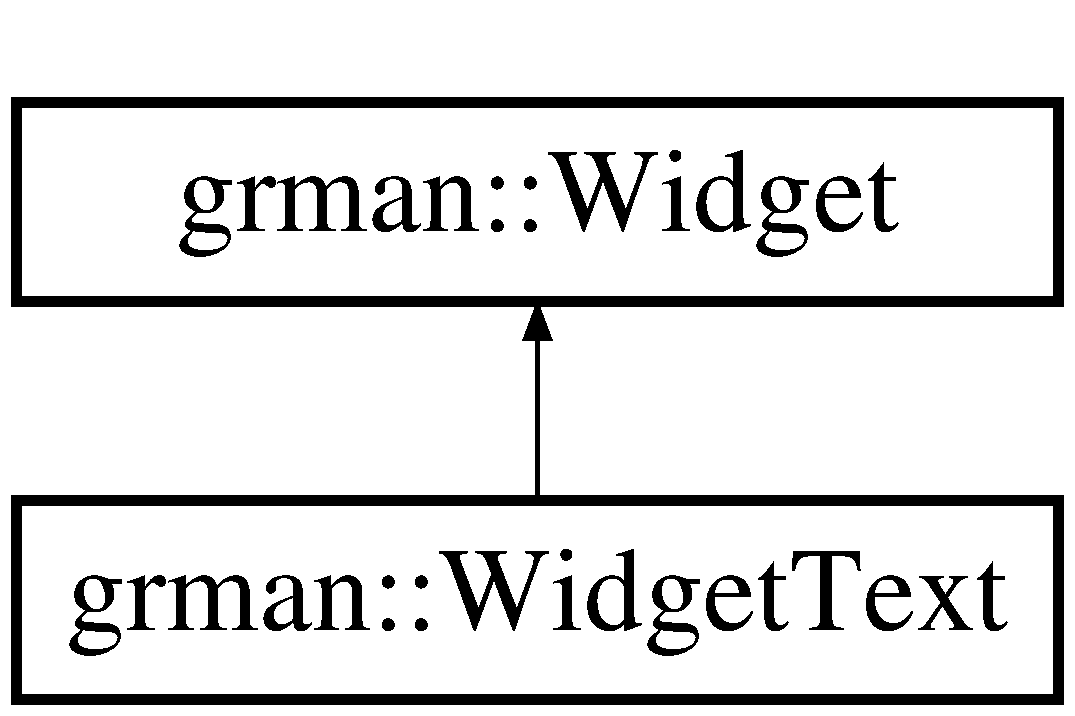
\includegraphics[height=2.000000cm]{classgrman_1_1_widget_text}
\end{center}
\end{figure}
\subsection*{Public Member Functions}
\begin{DoxyCompactItemize}
\item 
\mbox{\Hypertarget{classgrman_1_1_widget_text_a0d5ab6d804da36fdf0bcdb2a097edfc3}\label{classgrman_1_1_widget_text_a0d5ab6d804da36fdf0bcdb2a097edfc3}} 
{\bfseries Widget\+Text} (std\+::string message=\char`\"{}\char`\"{})
\item 
\mbox{\Hypertarget{classgrman_1_1_widget_text_af73e6a5dced3bd5ace8a99e0dd6c0e62}\label{classgrman_1_1_widget_text_af73e6a5dced3bd5ace8a99e0dd6c0e62}} 
virtual void \mbox{\hyperlink{classgrman_1_1_widget_text_af73e6a5dced3bd5ace8a99e0dd6c0e62}{draw}} ()
\begin{DoxyCompactList}\small\item\em Extr�mement rudimentaire \+: � compl�ter ! \end{DoxyCompactList}\item 
\mbox{\Hypertarget{classgrman_1_1_widget_text_a2b908c791e86834e8961b645cf835965}\label{classgrman_1_1_widget_text_a2b908c791e86834e8961b645cf835965}} 
void {\bfseries set\+\_\+message} (std\+::string message=\char`\"{}\char`\"{})
\item 
\mbox{\Hypertarget{classgrman_1_1_widget_text_aa18bd8b71ebf051c48535634d239e43c}\label{classgrman_1_1_widget_text_aa18bd8b71ebf051c48535634d239e43c}} 
std\+::string {\bfseries get\+\_\+message} ()
\item 
\mbox{\Hypertarget{classgrman_1_1_widget_text_a03b0b3cbba6184e076fbc7894771e99e}\label{classgrman_1_1_widget_text_a03b0b3cbba6184e076fbc7894771e99e}} 
void {\bfseries set\+\_\+vertical} (bool vertical=true)
\end{DoxyCompactItemize}
\subsection*{Protected Attributes}
\begin{DoxyCompactItemize}
\item 
\mbox{\Hypertarget{classgrman_1_1_widget_text_af4890cc8e49980454468109740dfe071}\label{classgrman_1_1_widget_text_af4890cc8e49980454468109740dfe071}} 
std\+::string {\bfseries m\+\_\+message}
\item 
\mbox{\Hypertarget{classgrman_1_1_widget_text_ae368be23564e5193942e4839ca78e913}\label{classgrman_1_1_widget_text_ae368be23564e5193942e4839ca78e913}} 
int {\bfseries m\+\_\+color} = N\+O\+IR
\item 
\mbox{\Hypertarget{classgrman_1_1_widget_text_a22c6d8eed2c019b48df545d83e4cf5e3}\label{classgrman_1_1_widget_text_a22c6d8eed2c019b48df545d83e4cf5e3}} 
F\+O\+NT $\ast$ {\bfseries m\+\_\+font} = font
\item 
\mbox{\Hypertarget{classgrman_1_1_widget_text_a854e398aea75d4030389a3788382a430}\label{classgrman_1_1_widget_text_a854e398aea75d4030389a3788382a430}} 
bool {\bfseries m\+\_\+vertical} = false
\end{DoxyCompactItemize}


\subsection{Detailed Description}
Extr�mement rudimentaire \+: � compl�ter ! 

Definition at line 213 of file widget.\+h.



The documentation for this class was generated from the following files\+:\begin{DoxyCompactItemize}
\item 
grman/widget.\+h\item 
grman/widget.\+cpp\end{DoxyCompactItemize}

\hypertarget{classgrman_1_1_widget_v_slider}{}\section{grman\+:\+:Widget\+V\+Slider Class Reference}
\label{classgrman_1_1_widget_v_slider}\index{grman\+::\+Widget\+V\+Slider@{grman\+::\+Widget\+V\+Slider}}
Inheritance diagram for grman\+:\+:Widget\+V\+Slider\+:\begin{figure}[H]
\begin{center}
\leavevmode
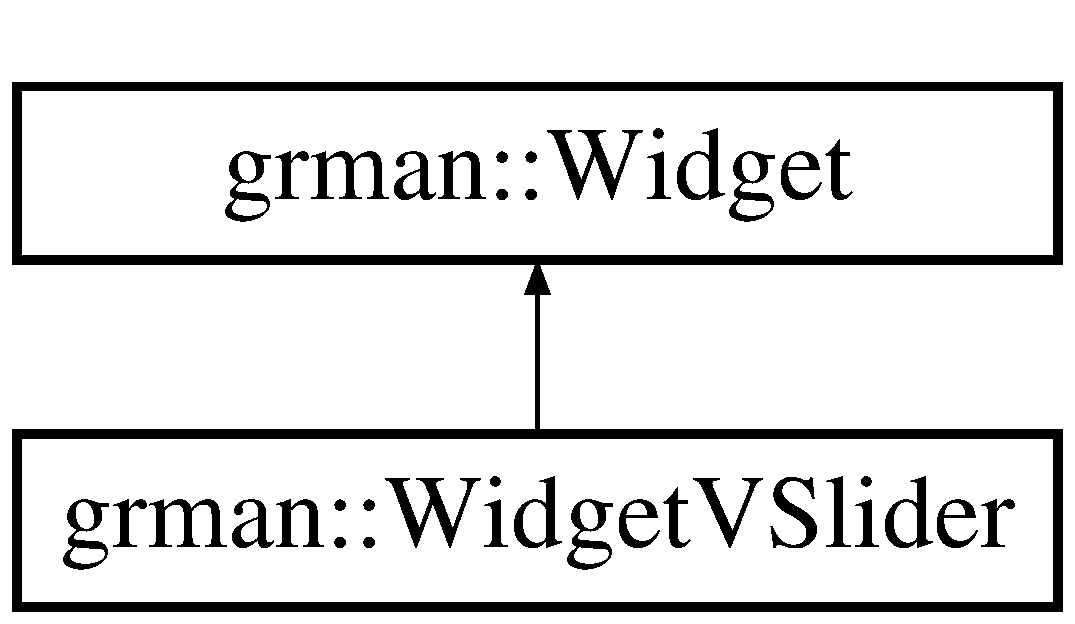
\includegraphics[height=2.000000cm]{classgrman_1_1_widget_v_slider}
\end{center}
\end{figure}
\subsection*{Public Member Functions}
\begin{DoxyCompactItemize}
\item 
\mbox{\Hypertarget{classgrman_1_1_widget_v_slider_a5c99012ba3a4c8df0764f6d9cdb04a04}\label{classgrman_1_1_widget_v_slider_a5c99012ba3a4c8df0764f6d9cdb04a04}} 
{\bfseries Widget\+V\+Slider} (double min=0, double max=99999, bool integer=false)
\item 
\mbox{\Hypertarget{classgrman_1_1_widget_v_slider_abe01c8a374090127186600950deeea1c}\label{classgrman_1_1_widget_v_slider_abe01c8a374090127186600950deeea1c}} 
virtual void {\bfseries draw} ()
\item 
\mbox{\Hypertarget{classgrman_1_1_widget_v_slider_a1045608d559b20463042553067b9eaa6}\label{classgrman_1_1_widget_v_slider_a1045608d559b20463042553067b9eaa6}} 
virtual void {\bfseries interact\+\_\+focus} ()
\item 
\mbox{\Hypertarget{classgrman_1_1_widget_v_slider_a31a7abe448a7a3f68e6fbc979af85aab}\label{classgrman_1_1_widget_v_slider_a31a7abe448a7a3f68e6fbc979af85aab}} 
virtual void {\bfseries interact\+\_\+over} ()
\item 
\mbox{\Hypertarget{classgrman_1_1_widget_v_slider_aefa232ab9252005f1d3d6dc560b39762}\label{classgrman_1_1_widget_v_slider_aefa232ab9252005f1d3d6dc560b39762}} 
virtual bool {\bfseries captures\+\_\+focus} ()
\item 
\mbox{\Hypertarget{classgrman_1_1_widget_v_slider_a2ff65cdbb07468558d5f1327dd3e3b15}\label{classgrman_1_1_widget_v_slider_a2ff65cdbb07468558d5f1327dd3e3b15}} 
double {\bfseries typed} (double v)
\item 
\mbox{\Hypertarget{classgrman_1_1_widget_v_slider_ae0462e56f0185a2841643f97a931206b}\label{classgrman_1_1_widget_v_slider_ae0462e56f0185a2841643f97a931206b}} 
double {\bfseries get\+\_\+value} ()
\item 
\mbox{\Hypertarget{classgrman_1_1_widget_v_slider_a4fa09e37283a46fef876c96ccf09cb6e}\label{classgrman_1_1_widget_v_slider_a4fa09e37283a46fef876c96ccf09cb6e}} 
void {\bfseries limit\+\_\+to\+\_\+range} ()
\item 
\mbox{\Hypertarget{classgrman_1_1_widget_v_slider_aeb7f889ce3cf0ca948fe79817b25181d}\label{classgrman_1_1_widget_v_slider_aeb7f889ce3cf0ca948fe79817b25181d}} 
void {\bfseries set\+\_\+value} (double value)
\item 
\mbox{\Hypertarget{classgrman_1_1_widget_v_slider_a379482a4d66b8bedfc84f76cfd8bddb3}\label{classgrman_1_1_widget_v_slider_a379482a4d66b8bedfc84f76cfd8bddb3}} 
void {\bfseries set\+\_\+range} (double min, double max, bool integer=false)
\end{DoxyCompactItemize}
\subsection*{Protected Member Functions}
\begin{DoxyCompactItemize}
\item 
\mbox{\Hypertarget{classgrman_1_1_widget_v_slider_a4f1b70003e9cb3e1355374c7b2dd47b2}\label{classgrman_1_1_widget_v_slider_a4f1b70003e9cb3e1355374c7b2dd47b2}} 
int {\bfseries get\+\_\+hhandle} ()
\end{DoxyCompactItemize}
\subsection*{Protected Attributes}
\begin{DoxyCompactItemize}
\item 
\mbox{\Hypertarget{classgrman_1_1_widget_v_slider_a5515dac66009ce6b5ab43bb9b7949d69}\label{classgrman_1_1_widget_v_slider_a5515dac66009ce6b5ab43bb9b7949d69}} 
double {\bfseries m\+\_\+value} = 0
\item 
\mbox{\Hypertarget{classgrman_1_1_widget_v_slider_a61be86890020cf9cd9a52f5bd80fed8a}\label{classgrman_1_1_widget_v_slider_a61be86890020cf9cd9a52f5bd80fed8a}} 
double {\bfseries m\+\_\+min}
\item 
\mbox{\Hypertarget{classgrman_1_1_widget_v_slider_afeeb86838c0237495bd581994b975ad3}\label{classgrman_1_1_widget_v_slider_afeeb86838c0237495bd581994b975ad3}} 
double {\bfseries m\+\_\+max}
\item 
\mbox{\Hypertarget{classgrman_1_1_widget_v_slider_ad3517557b287e27878b54fa730fc83e4}\label{classgrman_1_1_widget_v_slider_ad3517557b287e27878b54fa730fc83e4}} 
bool {\bfseries m\+\_\+integer}
\item 
\mbox{\Hypertarget{classgrman_1_1_widget_v_slider_a8b13d018065b9e59ce53619dcf5e9882}\label{classgrman_1_1_widget_v_slider_a8b13d018065b9e59ce53619dcf5e9882}} 
double {\bfseries m\+\_\+handle\+\_\+ratio} = .\+5
\item 
\mbox{\Hypertarget{classgrman_1_1_widget_v_slider_af4b78db8b06c7793d3ab9ce24acb47d0}\label{classgrman_1_1_widget_v_slider_af4b78db8b06c7793d3ab9ce24acb47d0}} 
double {\bfseries m\+\_\+rail\+\_\+ratio} = .\+3
\item 
\mbox{\Hypertarget{classgrman_1_1_widget_v_slider_abf4bcbc737d34bc4ef70be86c32803bb}\label{classgrman_1_1_widget_v_slider_abf4bcbc737d34bc4ef70be86c32803bb}} 
double {\bfseries m\+\_\+specific\+\_\+padding} = 2
\item 
\mbox{\Hypertarget{classgrman_1_1_widget_v_slider_a87a842c3b47b605d50eed6809e11893b}\label{classgrman_1_1_widget_v_slider_a87a842c3b47b605d50eed6809e11893b}} 
int {\bfseries m\+\_\+rail\+\_\+color} = G\+R\+IS
\item 
\mbox{\Hypertarget{classgrman_1_1_widget_v_slider_a897626a845e891c5c52069359848634c}\label{classgrman_1_1_widget_v_slider_a897626a845e891c5c52069359848634c}} 
int {\bfseries m\+\_\+handle\+\_\+color} = G\+R\+I\+S\+S\+O\+M\+B\+RE
\end{DoxyCompactItemize}


\subsection{Detailed Description}


Definition at line 278 of file widget.\+h.



The documentation for this class was generated from the following files\+:\begin{DoxyCompactItemize}
\item 
grman/widget.\+h\item 
grman/widget.\+cpp\end{DoxyCompactItemize}

\chapter{File Documentation}
\hypertarget{_edge_8cpp}{}\section{Edge.\+cpp File Reference}
\label{_edge_8cpp}\index{Edge.\+cpp@{Edge.\+cpp}}


Cr�ation d\textquotesingle{}un �cosyst�me.  


{\ttfamily \#include \char`\"{}Edge.\+h\char`\"{}}\newline


\subsection{Detailed Description}
Cr�ation d\textquotesingle{}un �cosyst�me. 

\begin{DoxyAuthor}{Author}
Groupe A\+G\+O\+U\+G\+I\+L\+E-\/\+C\+A\+M\+U\+G\+L\+I-\/\+A\+V\+A\+K\+I\+AN 
\end{DoxyAuthor}
\begin{DoxyVersion}{Version}
1.\+1 
\end{DoxyVersion}

\hypertarget{_edge_8h}{}\section{Edge.\+h File Reference}
\label{_edge_8h}\index{Edge.\+h@{Edge.\+h}}


Cr�ation d\textquotesingle{}un �cosyst�me.  


{\ttfamily \#include \char`\"{}Edge\+Interface.\+h\char`\"{}}\newline
\subsection*{Classes}
\begin{DoxyCompactItemize}
\item 
class \mbox{\hyperlink{class_edge}{Edge}}
\begin{DoxyCompactList}\small\item\em classe representant les arcs du graphe \end{DoxyCompactList}\end{DoxyCompactItemize}


\subsection{Detailed Description}
Cr�ation d\textquotesingle{}un �cosyst�me. 

\begin{DoxyAuthor}{Author}
Groupe A\+G\+O\+U\+G\+I\+L\+E-\/\+C\+A\+M\+U\+G\+L\+I-\/\+A\+V\+A\+K\+I\+AN 
\end{DoxyAuthor}
\begin{DoxyVersion}{Version}
1.\+1 
\end{DoxyVersion}

\hypertarget{_edge_interface_8cpp}{}\section{Edge\+Interface.\+cpp File Reference}
\label{_edge_interface_8cpp}\index{Edge\+Interface.\+cpp@{Edge\+Interface.\+cpp}}


Cr�ation d\textquotesingle{}un �cosyst�me.  


{\ttfamily \#include \char`\"{}Edge\+Interface.\+h\char`\"{}}\newline


\subsection{Detailed Description}
Cr�ation d\textquotesingle{}un �cosyst�me. 

\begin{DoxyAuthor}{Author}
Groupe A\+G\+O\+U\+G\+I\+L\+E-\/\+C\+A\+M\+U\+G\+L\+I-\/\+A\+V\+A\+K\+I\+AN 
\end{DoxyAuthor}
\begin{DoxyVersion}{Version}
1.\+1 
\end{DoxyVersion}

\hypertarget{_edge_interface_8h}{}\section{Edge\+Interface.\+h File Reference}
\label{_edge_interface_8h}\index{Edge\+Interface.\+h@{Edge\+Interface.\+h}}


Cr�ation d\textquotesingle{}un �cosyst�me.  


{\ttfamily \#include \char`\"{}grman/grman.\+h\char`\"{}}\newline
{\ttfamily \#include \char`\"{}Vertex.\+h\char`\"{}}\newline
\subsection*{Classes}
\begin{DoxyCompactItemize}
\item 
class \mbox{\hyperlink{class_edge_interface}{Edge\+Interface}}
\begin{DoxyCompactList}\small\item\em classe representant l\textquotesingle{}interface graphique des arcs du graphe \end{DoxyCompactList}\end{DoxyCompactItemize}


\subsection{Detailed Description}
Cr�ation d\textquotesingle{}un �cosyst�me. 

\begin{DoxyAuthor}{Author}
Groupe A\+G\+O\+U\+G\+I\+L\+E-\/\+C\+A\+M\+U\+G\+L\+I-\/\+A\+V\+A\+K\+I\+AN 
\end{DoxyAuthor}
\begin{DoxyVersion}{Version}
1.\+1 
\end{DoxyVersion}

\hypertarget{graph_8cpp}{}\section{graph.\+cpp File Reference}
\label{graph_8cpp}\index{graph.\+cpp@{graph.\+cpp}}


Cr�ation d\textquotesingle{}un �cosyst�me.  


{\ttfamily \#include \char`\"{}graph.\+h\char`\"{}}\newline


\subsection{Detailed Description}
Cr�ation d\textquotesingle{}un �cosyst�me. 

\begin{DoxyAuthor}{Author}
Groupe A\+G\+O\+U\+G\+I\+L\+E-\/\+C\+A\+M\+U\+G\+L\+I-\/\+A\+V\+A\+K\+I\+AN 
\end{DoxyAuthor}
\begin{DoxyVersion}{Version}
1.\+1 
\end{DoxyVersion}

\hypertarget{graph_8h}{}\section{graph.\+h File Reference}
\label{graph_8h}\index{graph.\+h@{graph.\+h}}


Cr�ation d\textquotesingle{}un �cosyst�me.  


{\ttfamily \#include $<$map$>$}\newline
{\ttfamily \#include $<$string$>$}\newline
{\ttfamily \#include \char`\"{}Edge.\+h\char`\"{}}\newline
{\ttfamily \#include \char`\"{}Graphe\+Interface.\+h\char`\"{}}\newline
{\ttfamily \#include $<$fstream$>$}\newline
{\ttfamily \#include $<$stack$>$}\newline
{\ttfamily \#include $<$vector$>$}\newline
{\ttfamily \#include $<$queue$>$}\newline
\subsection*{Classes}
\begin{DoxyCompactItemize}
\item 
class \mbox{\hyperlink{class_graph}{Graph}}
\begin{DoxyCompactList}\small\item\em classe representant le graphe \end{DoxyCompactList}\end{DoxyCompactItemize}


\subsection{Detailed Description}
Cr�ation d\textquotesingle{}un �cosyst�me. 

\begin{DoxyAuthor}{Author}
Groupe A\+G\+O\+U\+G\+I\+L\+E-\/\+C\+A\+M\+U\+G\+L\+I-\/\+A\+V\+A\+K\+I\+AN 
\end{DoxyAuthor}
\begin{DoxyVersion}{Version}
1.\+1 
\end{DoxyVersion}

\hypertarget{_graphe_interface_8cpp}{}\section{Graphe\+Interface.\+cpp File Reference}
\label{_graphe_interface_8cpp}\index{Graphe\+Interface.\+cpp@{Graphe\+Interface.\+cpp}}


Cr�ation d\textquotesingle{}un �cosyst�me.  


{\ttfamily \#include \char`\"{}Graphe\+Interface.\+h\char`\"{}}\newline


\subsection{Detailed Description}
Cr�ation d\textquotesingle{}un �cosyst�me. 

\begin{DoxyAuthor}{Author}
Groupe A\+G\+O\+U\+G\+I\+L\+E-\/\+C\+A\+M\+U\+G\+L\+I-\/\+A\+V\+A\+K\+I\+AN 
\end{DoxyAuthor}
\begin{DoxyVersion}{Version}
1.\+1 
\end{DoxyVersion}

\hypertarget{_graphe_interface_8h}{}\section{Graphe\+Interface.\+h File Reference}
\label{_graphe_interface_8h}\index{Graphe\+Interface.\+h@{Graphe\+Interface.\+h}}


Cr�ation d\textquotesingle{}un �cosyst�me.  


{\ttfamily \#include \char`\"{}grman/grman.\+h\char`\"{}}\newline
{\ttfamily \#include $<$string$>$}\newline
{\ttfamily \#include $<$vector$>$}\newline
{\ttfamily \#include \char`\"{}Edge.\+h\char`\"{}}\newline
\subsection*{Classes}
\begin{DoxyCompactItemize}
\item 
class \mbox{\hyperlink{class_graph_interface}{Graph\+Interface}}
\end{DoxyCompactItemize}


\subsection{Detailed Description}
Cr�ation d\textquotesingle{}un �cosyst�me. 

\begin{DoxyAuthor}{Author}
Groupe A\+G\+O\+U\+G\+I\+L\+E-\/\+C\+A\+M\+U\+G\+L\+I-\/\+A\+V\+A\+K\+I\+AN 
\end{DoxyAuthor}
\begin{DoxyVersion}{Version}
1.\+1 
\end{DoxyVersion}

\hypertarget{main_8cpp}{}\section{main.\+cpp File Reference}
\label{main_8cpp}\index{main.\+cpp@{main.\+cpp}}


Cr�ation d\textquotesingle{}un �cosyst�me.  


{\ttfamily \#include \char`\"{}grman/grman.\+h\char`\"{}}\newline
{\ttfamily \#include $<$iostream$>$}\newline
{\ttfamily \#include \char`\"{}graph.\+h\char`\"{}}\newline
{\ttfamily \#include \char`\"{}Acceuil1.\+h\char`\"{}}\newline
{\ttfamily \#include \char`\"{}Simulation.\+h\char`\"{}}\newline
{\ttfamily \#include \char`\"{}Analyse\+\_\+\+F\+\_\+\+C.\+h\char`\"{}}\newline
{\ttfamily \#include \char`\"{}Acceuil2.\+h\char`\"{}}\newline
{\ttfamily \#include \char`\"{}analyse\+\_\+\+K\+\_\+\+C.\+h\char`\"{}}\newline
\subsection*{Functions}
\begin{DoxyCompactItemize}
\item 
int \mbox{\hyperlink{main_8cpp_ae66f6b31b5ad750f1fe042a706a4e3d4}{main}} ()
\item 
\mbox{\Hypertarget{main_8cpp_ae5ce30f43c1f65cf5e459ac242938867}\label{main_8cpp_ae5ce30f43c1f65cf5e459ac242938867}} 
{\bfseries E\+N\+D\+\_\+\+O\+F\+\_\+\+M\+A\+IN} ()
\end{DoxyCompactItemize}


\subsection{Detailed Description}
Cr�ation d\textquotesingle{}un �cosyst�me. 

\begin{DoxyAuthor}{Author}
Groupe A\+G\+O\+U\+G\+I\+L\+E-\/\+C\+A\+M\+U\+G\+L\+I-\/\+A\+V\+A\+K\+I\+AN 
\end{DoxyAuthor}
\begin{DoxyVersion}{Version}
1.\+1 
\end{DoxyVersion}


\subsection{Function Documentation}
\mbox{\Hypertarget{main_8cpp_ae66f6b31b5ad750f1fe042a706a4e3d4}\label{main_8cpp_ae66f6b31b5ad750f1fe042a706a4e3d4}} 
\index{main.\+cpp@{main.\+cpp}!main@{main}}
\index{main@{main}!main.\+cpp@{main.\+cpp}}
\subsubsection{\texorpdfstring{main()}{main()}}
{\footnotesize\ttfamily int main (\begin{DoxyParamCaption}{ }\end{DoxyParamCaption})}

A appeler en 1er avant d\textquotesingle{}instancier des objets graphiques etc..t.

Le nom du r�pertoire o� se trouvent les images � charger

Un exemple de graphe

g.\+Tuer\+Sommet(5);



 D�but Forte conexit� 





 F\+IN Forte conexit� 



clear le graphe

recharger le graphe 

Definition at line 19 of file main.\+cpp.


\hypertarget{_vertex_8cpp}{}\section{Vertex.\+cpp File Reference}
\label{_vertex_8cpp}\index{Vertex.\+cpp@{Vertex.\+cpp}}


Cr�ation d\textquotesingle{}un �cosyst�me.  


{\ttfamily \#include \char`\"{}Vertex.\+h\char`\"{}}\newline


\subsection{Detailed Description}
Cr�ation d\textquotesingle{}un �cosyst�me. 

\begin{DoxyAuthor}{Author}
Groupe A\+G\+O\+U\+G\+I\+L\+E-\/\+C\+A\+M\+U\+G\+L\+I-\/\+A\+V\+A\+K\+I\+AN 
\end{DoxyAuthor}
\begin{DoxyVersion}{Version}
1.\+1 
\end{DoxyVersion}

\hypertarget{_vertex_8h}{}\section{Vertex.\+h File Reference}
\label{_vertex_8h}\index{Vertex.\+h@{Vertex.\+h}}


Cr�ation d\textquotesingle{}un �cosyst�me.  


{\ttfamily \#include $<$vector$>$}\newline
{\ttfamily \#include $<$memory$>$}\newline
{\ttfamily \#include \char`\"{}Vertex\+Interface.\+h\char`\"{}}\newline
\subsection*{Classes}
\begin{DoxyCompactItemize}
\item 
class \mbox{\hyperlink{class_vertex}{Vertex}}
\begin{DoxyCompactList}\small\item\em classe representant les sommets du graphe \end{DoxyCompactList}\end{DoxyCompactItemize}


\subsection{Detailed Description}
Cr�ation d\textquotesingle{}un �cosyst�me. 

\begin{DoxyAuthor}{Author}
Groupe A\+G\+O\+U\+G\+I\+L\+E-\/\+C\+A\+M\+U\+G\+L\+I-\/\+A\+V\+A\+K\+I\+AN 
\end{DoxyAuthor}
\begin{DoxyVersion}{Version}
1.\+1 
\end{DoxyVersion}

\hypertarget{_vertex_interface_8cpp}{}\section{Vertex\+Interface.\+cpp File Reference}
\label{_vertex_interface_8cpp}\index{Vertex\+Interface.\+cpp@{Vertex\+Interface.\+cpp}}


Cr�ation d\textquotesingle{}un �cosyst�me.  


{\ttfamily \#include \char`\"{}Vertex\+Interface.\+h\char`\"{}}\newline


\subsection{Detailed Description}
Cr�ation d\textquotesingle{}un �cosyst�me. 

\begin{DoxyAuthor}{Author}
Groupe A\+G\+O\+U\+G\+I\+L\+E-\/\+C\+A\+M\+U\+G\+L\+I-\/\+A\+V\+A\+K\+I\+AN 
\end{DoxyAuthor}
\begin{DoxyVersion}{Version}
1.\+1 
\end{DoxyVersion}

\hypertarget{_vertex_interface_8h}{}\section{Vertex\+Interface.\+h File Reference}
\label{_vertex_interface_8h}\index{Vertex\+Interface.\+h@{Vertex\+Interface.\+h}}


Cr�ation d\textquotesingle{}un �cosyst�me.  


{\ttfamily \#include \char`\"{}grman/grman.\+h\char`\"{}}\newline
\subsection*{Classes}
\begin{DoxyCompactItemize}
\item 
class \mbox{\hyperlink{class_vertex_interface}{Vertex\+Interface}}
\begin{DoxyCompactList}\small\item\em classe representant l\textquotesingle{}interface graphique des sommets \end{DoxyCompactList}\end{DoxyCompactItemize}


\subsection{Detailed Description}
Cr�ation d\textquotesingle{}un �cosyst�me. 

\begin{DoxyAuthor}{Author}
Groupe A\+G\+O\+U\+G\+I\+L\+E-\/\+C\+A\+M\+U\+G\+L\+I-\/\+A\+V\+A\+K\+I\+AN 
\end{DoxyAuthor}
\begin{DoxyVersion}{Version}
1.\+1 
\end{DoxyVersion}

%--- End generated contents ---

% Index
\backmatter
\newpage
\phantomsection
\clearemptydoublepage
\addcontentsline{toc}{chapter}{Index}
\printindex

\end{document}
